% !BIB TS-program = biber

\RequirePackage[l2tabu,orthodox]{nag}

% TODO: decide if one-sided/two-sided
%\documentclass[headsepline,footsepline,footinclude=false,fontsize=11pt,paper=a4,listof=totoc,bibliography=totoc,BCOR=12mm,DIV=12]{scrbook} % two-sided
\documentclass[headsepline,footsepline,footinclude=false,oneside,fontsize=11pt,paper=a4,listof=totoc,bibliography=totoc]{scrbook} % one-sided

\newcommand*{\getUniversity}{Technische Universität München}
\newcommand*{\getFaculty}{Informatics}
\newcommand*{\getDegree}{Informatics}
\newcommand*{\getSchool}{Computation, Information and Technology}
\newcommand*{\getTitle}{Comparative Analysis of Widely Used Zipfian Distribution Implementations}
\newcommand*{\getTitleGer}{Vergleichende Analyse von häufig verwendenten Implementierungen der Zipf-Verteilung}
\newcommand*{\getAuthor}{Rodrigo Felix Forno}
\newcommand*{\getDoctype}{Bachelor's Thesis}
\newcommand*{\getSupervisor}{Prof. Dr. Viktor Leis}
\newcommand*{\getAdvisor}{Bohyun Lee M.Sc., Gabriel Haas M.Sc.}
\newcommand*{\getKeywords}{keyword;another keyword;one more}
\newcommand*{\getSubmissionDate}{25th of March, 2025}
\newcommand*{\getSubmissionLocation}{Munich}

\input{settings}

\begin{document}

% Set page numbering to avoid "destination with the same identifier has been already used" warning for cover page.
% (see https://en.wikibooks.org/wiki/LaTeX/Hyperlinks#Problems_with_Links_and_Pages).
\pagenumbering{alph}
\input{pages/cover}

\frontmatter{}

\input{pages/title}
\input{pages/disclaimer}
\chapter{\abstractname}

%TODO: Abstract
This thesis analysis common implementations of sampling algorithms used to generate variates of the Zipfian distribution, with special attention given
to the use cases found in storage systems and database technology research. Since the late eighties, there has been increased interest in evaluating the performance
of those systems under very skewed workloads, which are often modeled using the Zipfian distribution. While the theory behind some sampling techniques for the Zipfian distribution is well grounded, 
practical implementations vary in their accuracy and performance, which can lead to incorrect results in the evaluation of storage systems. This work presents a comprehensive analysis of the most common sampling algorithms 
found in benchmarking suites across academia and industry, and offers a comparison in terms of precision, speed and applicability to the aforementioned research areas. Parallely, two programs were written to help analysis: a benchmark tool was developed to run experiments on different implementations and
implementation of different variate generators was done in the programming language C++. Evaluation shows that most found implementations are suitable for the use cases in storage systems and database technology research, but some, such as FIO, are to be avoided. 
It was also revealed that table lookups might be an interesting alternative to established method, but further investigation is required.
\microtypesetup{protrusion=false}
\tableofcontents{}
\microtypesetup{protrusion=true}

\mainmatter{}

% !TeX root = ../main.tex
% Add the above to each chapter to make compiling the PDF easier in some editors.

\chapter{Introduction}\label{chapter:introduction}

The Zipfian distribution is a power law that has been observed in a wide range of natural and artificial phenomena. 
It is characterized by the fact that the frequency of an element is inversely proportional to its rank, meaning the position of the element in the sorted list of elements.
A quick example makes this principle quite clear.

\begin{figure}[ht!]
  \centering
  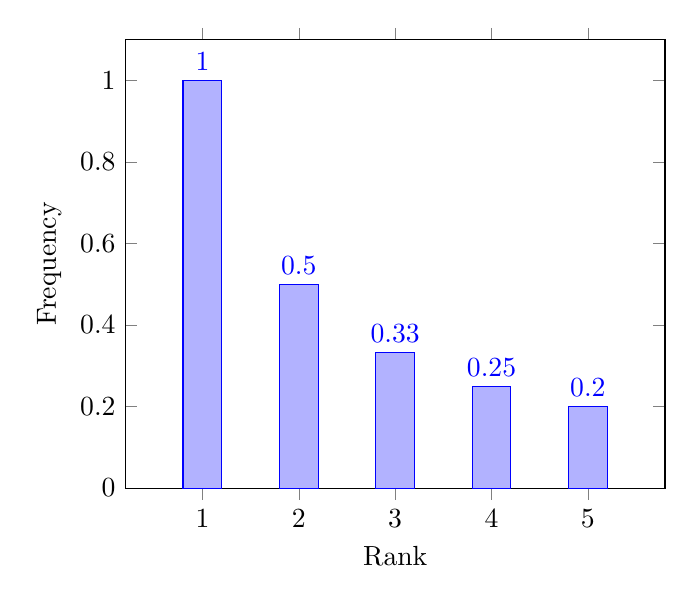
\begin{tikzpicture}
  \begin{axis}[
    ybar,
    bar width=14pt,
    enlarge x limits=0.2,
    symbolic x coords={1,2,3,4,5},
    xtick=data,
    xlabel={Rank},
    ylabel={Frequency},
    ymin=0, ymax=1.1,
    nodes near coords,
    ]
    \addplot coordinates {
      (1,1)     
      (2,0.5)   
      (3,0.333) 
      (4,0.25)   
      (5,0.2)    
    };
  \end{axis}
\end{tikzpicture}

  \caption{Example of a Zipfian distribution}
  \label{fig:zipf_example} 
\end{figure}

This means that the most frequent element is twice as frequent as the second most frequent element, three times as frequent as the third most frequent element, and so on. 
This distribution has been observed in a wide range of natural phenomena, such as the distribution of words in natural languages, the distribution of cities by population, among others \cite{mandelbrotNatureFractal1998}. And also within the fields of storage systems research, networking theory
as well as databases, there has been more compelling evidence that the Zipfian distribution (or more generally, heavy-tailed distributions) is a good model for the distribution of access patterns in these systems \cite{grayQuicklyGeneratingBillionrecord1994, crovellaPerformanceEvaluationHeavy2000,deanTailScale2013}.

The focus however of this thesis is on the large-scale generation of Zipfian samples, which are essential for the evaluation of latency and general performance in storage systems and databases. 
To this end, the state-of-the-art in synthetic workload generation is reviewed and common solutions are identified and evaluated. Parallely, a study of variate generation algorithms is conducted, with a focus on the generation of Zipfian variates.
This will allow for the comparison in terms of speed and accuracy of common implementations as well as give a baseline for an improved version. The main contributions of this thesis are:
\begin{itemize}
  \item A review of the state-of-the-art in synthetic workload generation, with a focus on the generation of Zipfian variates.
  \item A study of variate generation algorithms, with a focus on the generation of Zipfian variates.
  \item An implementation of a Zipfian variate generator in C++20, with a focus on performance and algorithmic simplicity
  \item An evaluation of the performance of the implemented Zipfian variate generator in comparison to existing solutions
\end{itemize}

The results show that existing solutions are generally accurate and fast, while one framework, FIO, is incorrect for larger sample sizes. One of the algorithms, \textit{Rejection-Inversion}, 
is still one of the fastest and the most accurate for generating variates of the target distribution, though table methods could present a new alternative if further optimized. Generally
implementations based in Java, with around $27$ million variates per second, were between $1.4$ and $1.8$ times slower than their C/C++ counterparts, with around $44$ million variates per second. 
As such, these implementations can still be recommended for synthetic workload generation. Furthermore accuracy analysis shows that the implementations found
in common benchmark suites are quite accurate: the ratio between sampled frequencies and theoretical ones are quite close to $1$ for sampel sizes $10$ times the support size while maximal
absolute error is around $10^{-3}$. It was also found out that the sampled distributions converge quite fast, with $10$ times the sample size being a good rule of thumb for the number of samples needed.

\chapter{Background}\label{chapter:background}

The Zipfian distribution (also known as \textit {Zipf's Law}
 \cite{powersApplicationsExplanationsZipfs1998a}) is a power law; that is, 
 the relationship between the probability of an event and the quantity that 
 describes the event 
is given by an exponential factor \cite{newmanPowerLawsPareto2005}. A simple example of a power law is the relationship of the \textit{area of a square}, $A(x)$, and its 
\textit{side length}, $x$, given by $A(x) = x^2$. A formal definition is given below, parametrized by what we will
define as the \textit{skew} - $\alpha$.

\begin{equation}
    f(x) = C \cdot x^\alpha
    \label{eq:power-law}
\end{equation}

\paragraph{Zipf's Law} While a power-law, Zipf's is slightly different
 than the area of a square in that it is defined as a set of discrete values.
  For instance, when parsing a text and collecting the number of occurrences of 
  each word, there are only finitely many words. The same occurs for databases: a key to a table has only a finite number of values. Moreover,
 the law says that the word rank - a word's position or key in terms of popularity -
  is inversely proportional to its frequency, given a skew factor. Formally, 
  it is defined as follows:

\begin{equation}\label{eqt:zm_law}
    \textbf{frequency} \propto \frac{1}{\textbf{rank}^\alpha}
\end{equation}

An example is given in Figure \ref{fig:zipf_example}. A text was parsed and a 
list of top five most popular words has been compiled: "the", "a", "an", "of", "to".
The frequency is defined to be $freq(word) = \frac{occurences(word)}{\sum_{all words} occurences(words)}$.
 We observe that the frequencies sum up to $1$, and that the relationship
between rank and frequency is not linear, but closely resembles an exponential 
curve. 

\begin{figure}[t]
  \centering
  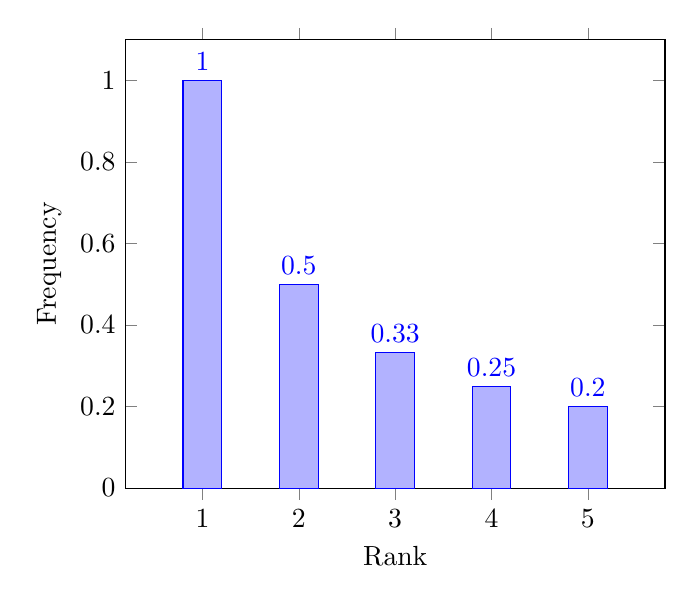
\begin{tikzpicture}
  \begin{axis}[
    ybar,
    bar width=14pt,
    enlarge x limits=0.2,
    symbolic x coords={1,2,3,4,5},
    xtick=data,
    xlabel={Rank},
    ylabel={Frequency},
    ymin=0, ymax=1.1,
    nodes near coords,
    ]
    \addplot coordinates {
      (1,1)     
      (2,0.5)   
      (3,0.333) 
      (4,0.25)   
      (5,0.2)    
    };
  \end{axis}
\end{tikzpicture}

  \caption{Example of a Zipfian distribution}
  \label{fig:zipf_example} 
\end{figure}

\paragraph{The generalized Zipfian} The previous example and intuition are helpful in 
understanding the pattern that this law presents, however, it is necessary to define 
it more deeply. From now on, the following conventions will be used:

\begin{itemize}
    \item $N$ - The support size of the distribution (e.g. \textit{number of different words})
    \item $k$ - The rank of the \textit{variate}\footnote{this is used interchangebly with \textit{sample}} (e.g. \textit{rank of word})
\end{itemize}

Since the aim is generating variates according to this law, it is necessary to
 treat the \textit{generalized Zipfian} as a statistical distribution. Below follows its
\ac{PMF}:
\begin{equation}\label{eqt:zm_prob}
    f(k, N, \alpha) := 
 \begin{cases} 
      \frac{1}{H_{N,\alpha}} \frac{1}{k^\alpha} & 1 \leq k \leq N \\
      0 & k < 1 \, \text{or} \, N < k 
   \end{cases}
\end{equation}

The term $H_{N,\alpha}$ is defined as the \textit{generalized harmonic number} \cite{newmanPowerLawsPareto2005}, acting as the normalizing constant $C$ 
seen in \ref{eq:power-law} and ensuring the \ac{PMF} sums to $1$. It is defined as:

\begin{equation}\label{eqt:generalized_hn}
    H_{N, \alpha} = \sum_{k = 1}^{N} \frac{1}{k^\alpha}
\end{equation}

As done before with Zipf's Law, the \textit{Zipfian} distribution is plotted in Figure \ref{fig:zipf_pmf} as a line plot, this time with a \textit{support size} of $100$ distinct words. 
Now that all relevant terms are defined, we turn to the original problem of generating \textit{samples}.

\begin{figure}[t]
    \centering
    \begin{tikzpicture}
    \begin{axis}[
        xlabel={$k$},
        ylabel={$P(X=k)$},
        grid=both,
        thick,
        ymin=0,
        ymax=0.2,
        xtick distance=10,
    ]
    
    \pgfplotstableread[col sep=comma]{data/zipf_pmf.csv}\datatable  
    \addplot table[x=k, y=PMF] {\datatable};
    \end{axis}
\end{tikzpicture}
    \caption{Probability Mass Function of a Zipfian distribution with $N = 100$ and $\alpha = 1$}
    \label{fig:zipf_pmf}
\end{figure}

\section{Discrete Variate Generation}
The goal of \textit{discrete variate generation} is to produce a set
 $\tilde{X}$ of $m$ variates contained in the \textit{support interval} $[0,N]$, 
 such that $freq(x_i) \sim Dist(\alpha)$ for $i \in [0,m]$. In other words,
  the samples follow a given distribution $Dist(\alpha)$. To achieve this, all sampling algorithms use 
an random \textit{uniform} distribution $U$, and transform  these uniform \textit{samples} into the 
target samples \cite{kuhlHistoryRandomVariate2017}. As distributions 
have different properties, some sampling methods are better than others for a particular distribution. Knowing this, the discussion is restricted to the algorithms listed below, as literature
confirms these methods are better than alternatives (see \cite{devroyeDiscreteUnivariateDistributions1986,kronmalAliasMethodGenerating1979,kuhlHistoryRandomVariate2017}).

\begin{enumerate}
    \item Rejection Sampling \cite{devroyeDiscreteUnivariateDistributions1986}
    \item Rejection-Inversion Sampling \cite{hormannRejectioninversionGenerateVariates1996}
    \item Condensed Table Lookup \cite{marsagliaFastGenerationDiscrete2004}
    \item Approximative sampling \cite{grayQuicklyGeneratingBillionrecord1994}
\end{enumerate}

The first two methods, \textit{Rejection Sampling} and \textit{Rejection-Inversion Sampling}, are \textbf{exact}, whereas the last two, \textit{Condensed Table Lookup}
and \textit{Approximative Sampling}, are \textbf{approximations}. Consequently, given enough samples, the first two should converge to a \textit{Zipfian} distribution if implemented correctly,
whereas the latter two might have systematic deviations \cite{leydoldErrorDetectionNonUniforma}. The following subsections will explain each algorithm.

\subsection{Rejection Sampling}\label{subsec:rejection_sampling}
Rejection sampling works by \textit{rejecting} samples from a \textit{uniform}
 distribution using a \textit{bounding function} to decide which samples are kept 
and which are thrown away. A good example is a dartboard, onto which darts are 
thrown at random. If the target distribution is normal, we draw its contour
(the \textit{bounding function}) in the dartboard and \textit{accept}
 the darts that fall below it and \textit{reject} the ones above. 
The graphs in Figure \ref{fig:rejection_sampling} illustrate this principle well 
- blue points are accepted darts, whereas red points are the rejected ones.

\begin{figure}[ht]
    \centering
    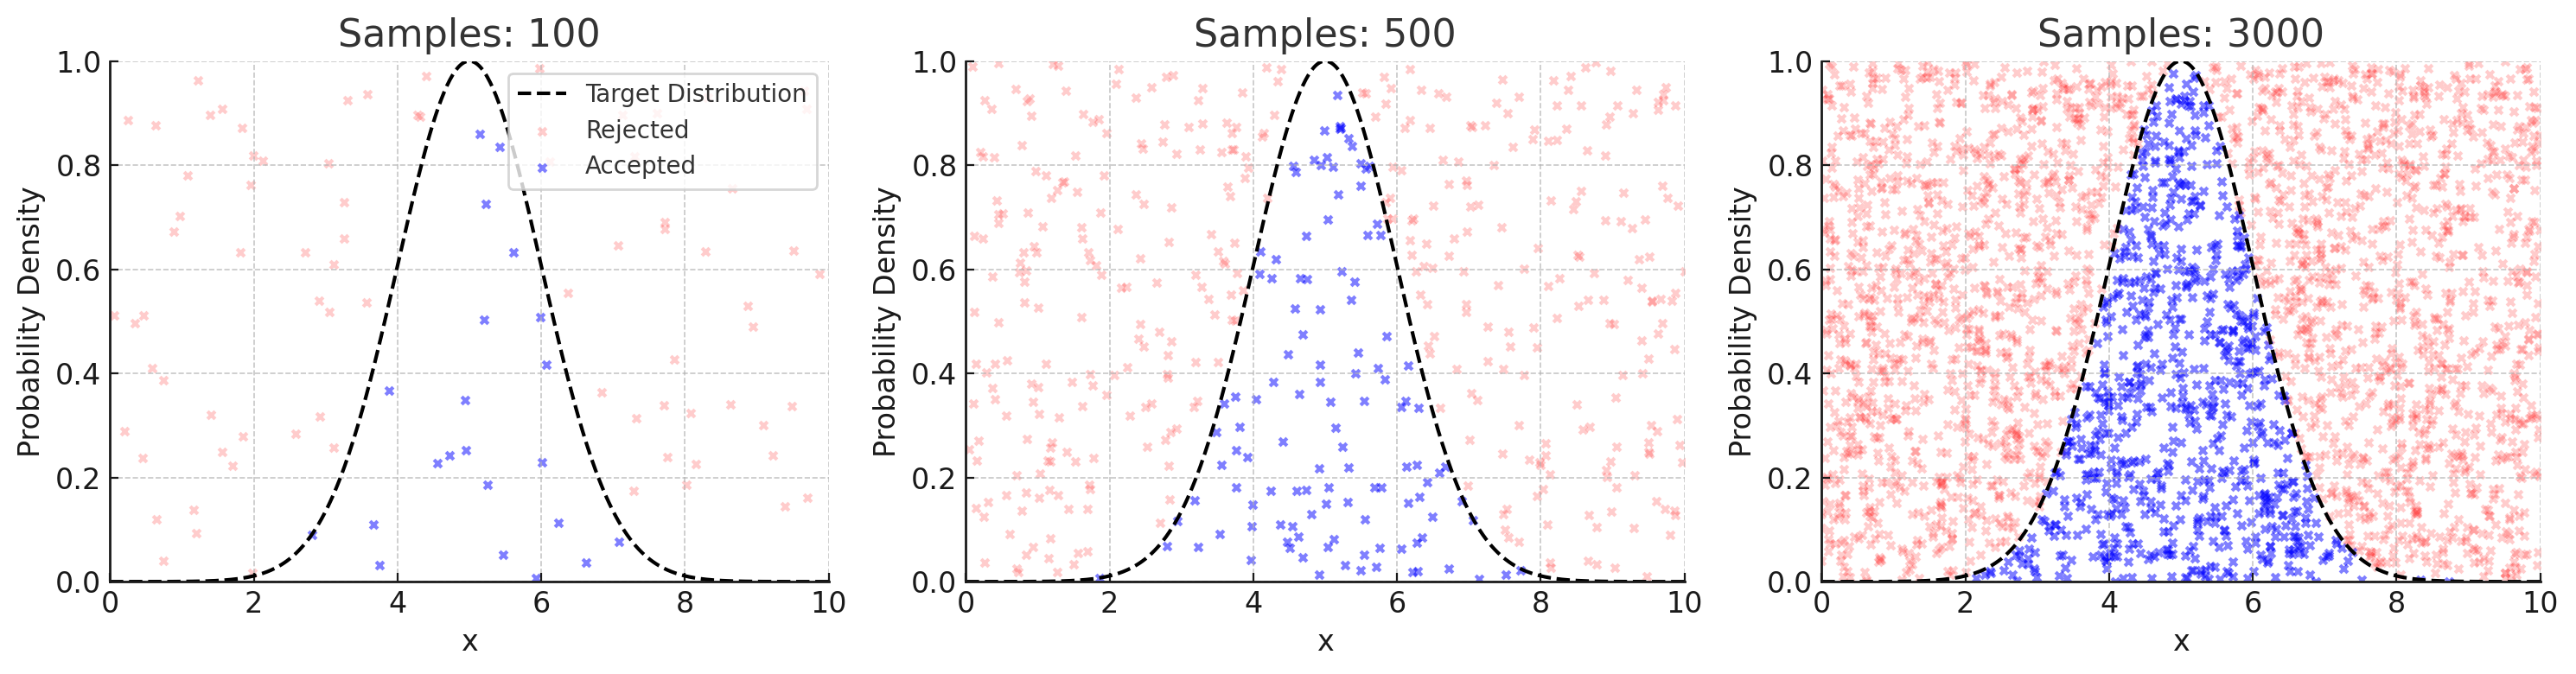
\includegraphics[width=\linewidth]{figures/rejection_sampling.png}
    \caption{To generate these graphs, a random uniform sample is taken for the x-axis as well as another normalized one for the y-axis.}\label{fig:rejection_sampling}
\end{figure}

Similar to the normal distribution, a \textit{bounding function} is chosen for the \textit{Zipfian}: $1/k^{-\alpha}$. This function is easier to determine than
the \ac{PMF} in Equation \ref{eqt:zm_prob}, as we skip the computationally expensive normalization constant. The only requirement on this function is that it should 
\textit{be greater up to a constant factor} than the original \ac{PMF}. A disadvantage of 
this method is that two random samples are required: one for the x-axis, another for the y-axis.

\subsection{Rejection-Inversion Sampling}\label{subsec:rejection_inversion}
Due to Hörmann and Derflinger \cite{hormannRejectioninversionGenerateVariates1996}, this method
 is a more efficient version of the Rejection Sampling method. 
It is based on the following observations regarding the naive rejection method:
\begin{itemize}
    \item A naive rejection algorithm requires two samples to generate the target variate.
    \item The Zipfian is bounded by a monotonically decreasing and convex function, which makes it possible to invert the bounding function.
\end{itemize}

These two observations lead to the following principle:

\vspace{0.3cm}

\fbox{
    \parbox{0.83\linewidth}{
        Generate a random variate $u$ from the uniform distribution $U(0,1)$ and invert the bounding function to find the corresponding $x = H^{-1}(u)$.
        Define a bounding area around the nearest integer $k$ (with radius $a$).
        Accept $X$ as a sample if $x \geq x_k$ and $x \leq k + a $. Otherwise, reject it.\footnotemark
    }
}
\footnotetext{This is a simplified version of the algorithm. For a more detailed explanation, see \cite{hormannRejectioninversionGenerateVariates1996}}
\vspace{0.3cm}

To visualize the principle used, consider Figure \ref{fig:rejection_inversion}: After $k$ was found using the inversion method, the bounding area is defined for radius $a$. 
Therefore an interval beginning at $k - a$ and ending at $k + a$ is defined, then used to accept or reject $x$. Typically, $a$ is chosen to be $1/2$ \cite{hormannRejectioninversionGenerateVariates1996}.

\begin{figure}[t]
    \centering
    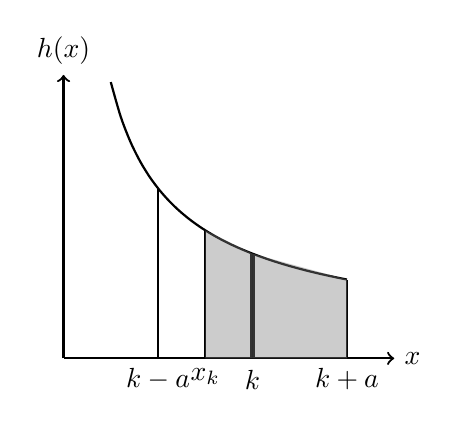
\begin{tikzpicture}[scale=1.2]
    % Axes
    \draw[thick,->] (0,0) -- (3.5,0) node[right] {$x$};
    \draw[thick,->] (0,0) -- (0,3) node[above] {$h(x)$};

    \draw[thick, domain=0.5:3, smooth, variable=\x] plot ({\x}, {1.8/\x^(0.7)});

    % Vertical lines
    \draw[thick] (1,0) node[below] {$k-a$} -- (1,{1.8});
    \draw[thick] (1.5,0) node[below] {$x_k$} -- (1.5,{1.8/(1.5^0.7)});
    \draw[ultra thick] (2,0) node[below] {$k$} -- (2,{1.8/(2^0.7)});
    \draw[thick] (3,0) node[below] {$k+a$} -- (3,{1.8/(3^0.7)});

    % Shaded areas (rejection and acceptance)
    \fill[gray,opacity=0.4] (1.5,0) -- (1.5,{1.8/(1.5^0.7)}) -- (2,{1.8/(2^0.7)}) -- (2,0) -- cycle;
    \fill[gray,opacity=0.4] (2,0) -- (2,{1.8/(2^0.7)}) -- (3,{1.8/(3^0.7)}) -- (3,0) -- cycle;

\end{tikzpicture}

    \caption{Rejection-Inversion Sampling for a Zipfian distribution}\label{fig:rejection_inversion}
\end{figure}

\subsection{Condensed Table Lookup}\label{subsec:condensed_table}
An alternative to exact methods is computing probabilities of a function according to a \ac{PMF} for all \textit{ranks} in the domain and storing them in a table. Since this 
probability is defined in an interval $[0,1]$, it is possible to take a random \textit{uniform} sample from the interval $[0,1]$ and look up the entry stored at the matching probability.
This sampling technique is called a \textit{table lookup} method \cite{marsagliaFastGenerationDiscrete2004}. Consider Figure \ref{fig:lookup_table}: 
A sample from an \textit{uniform} distribution (the implementation is a \ac{PRNG}) is taken and used to find the corresponding index in the table.

\begin{figure}[h]
    \centering
    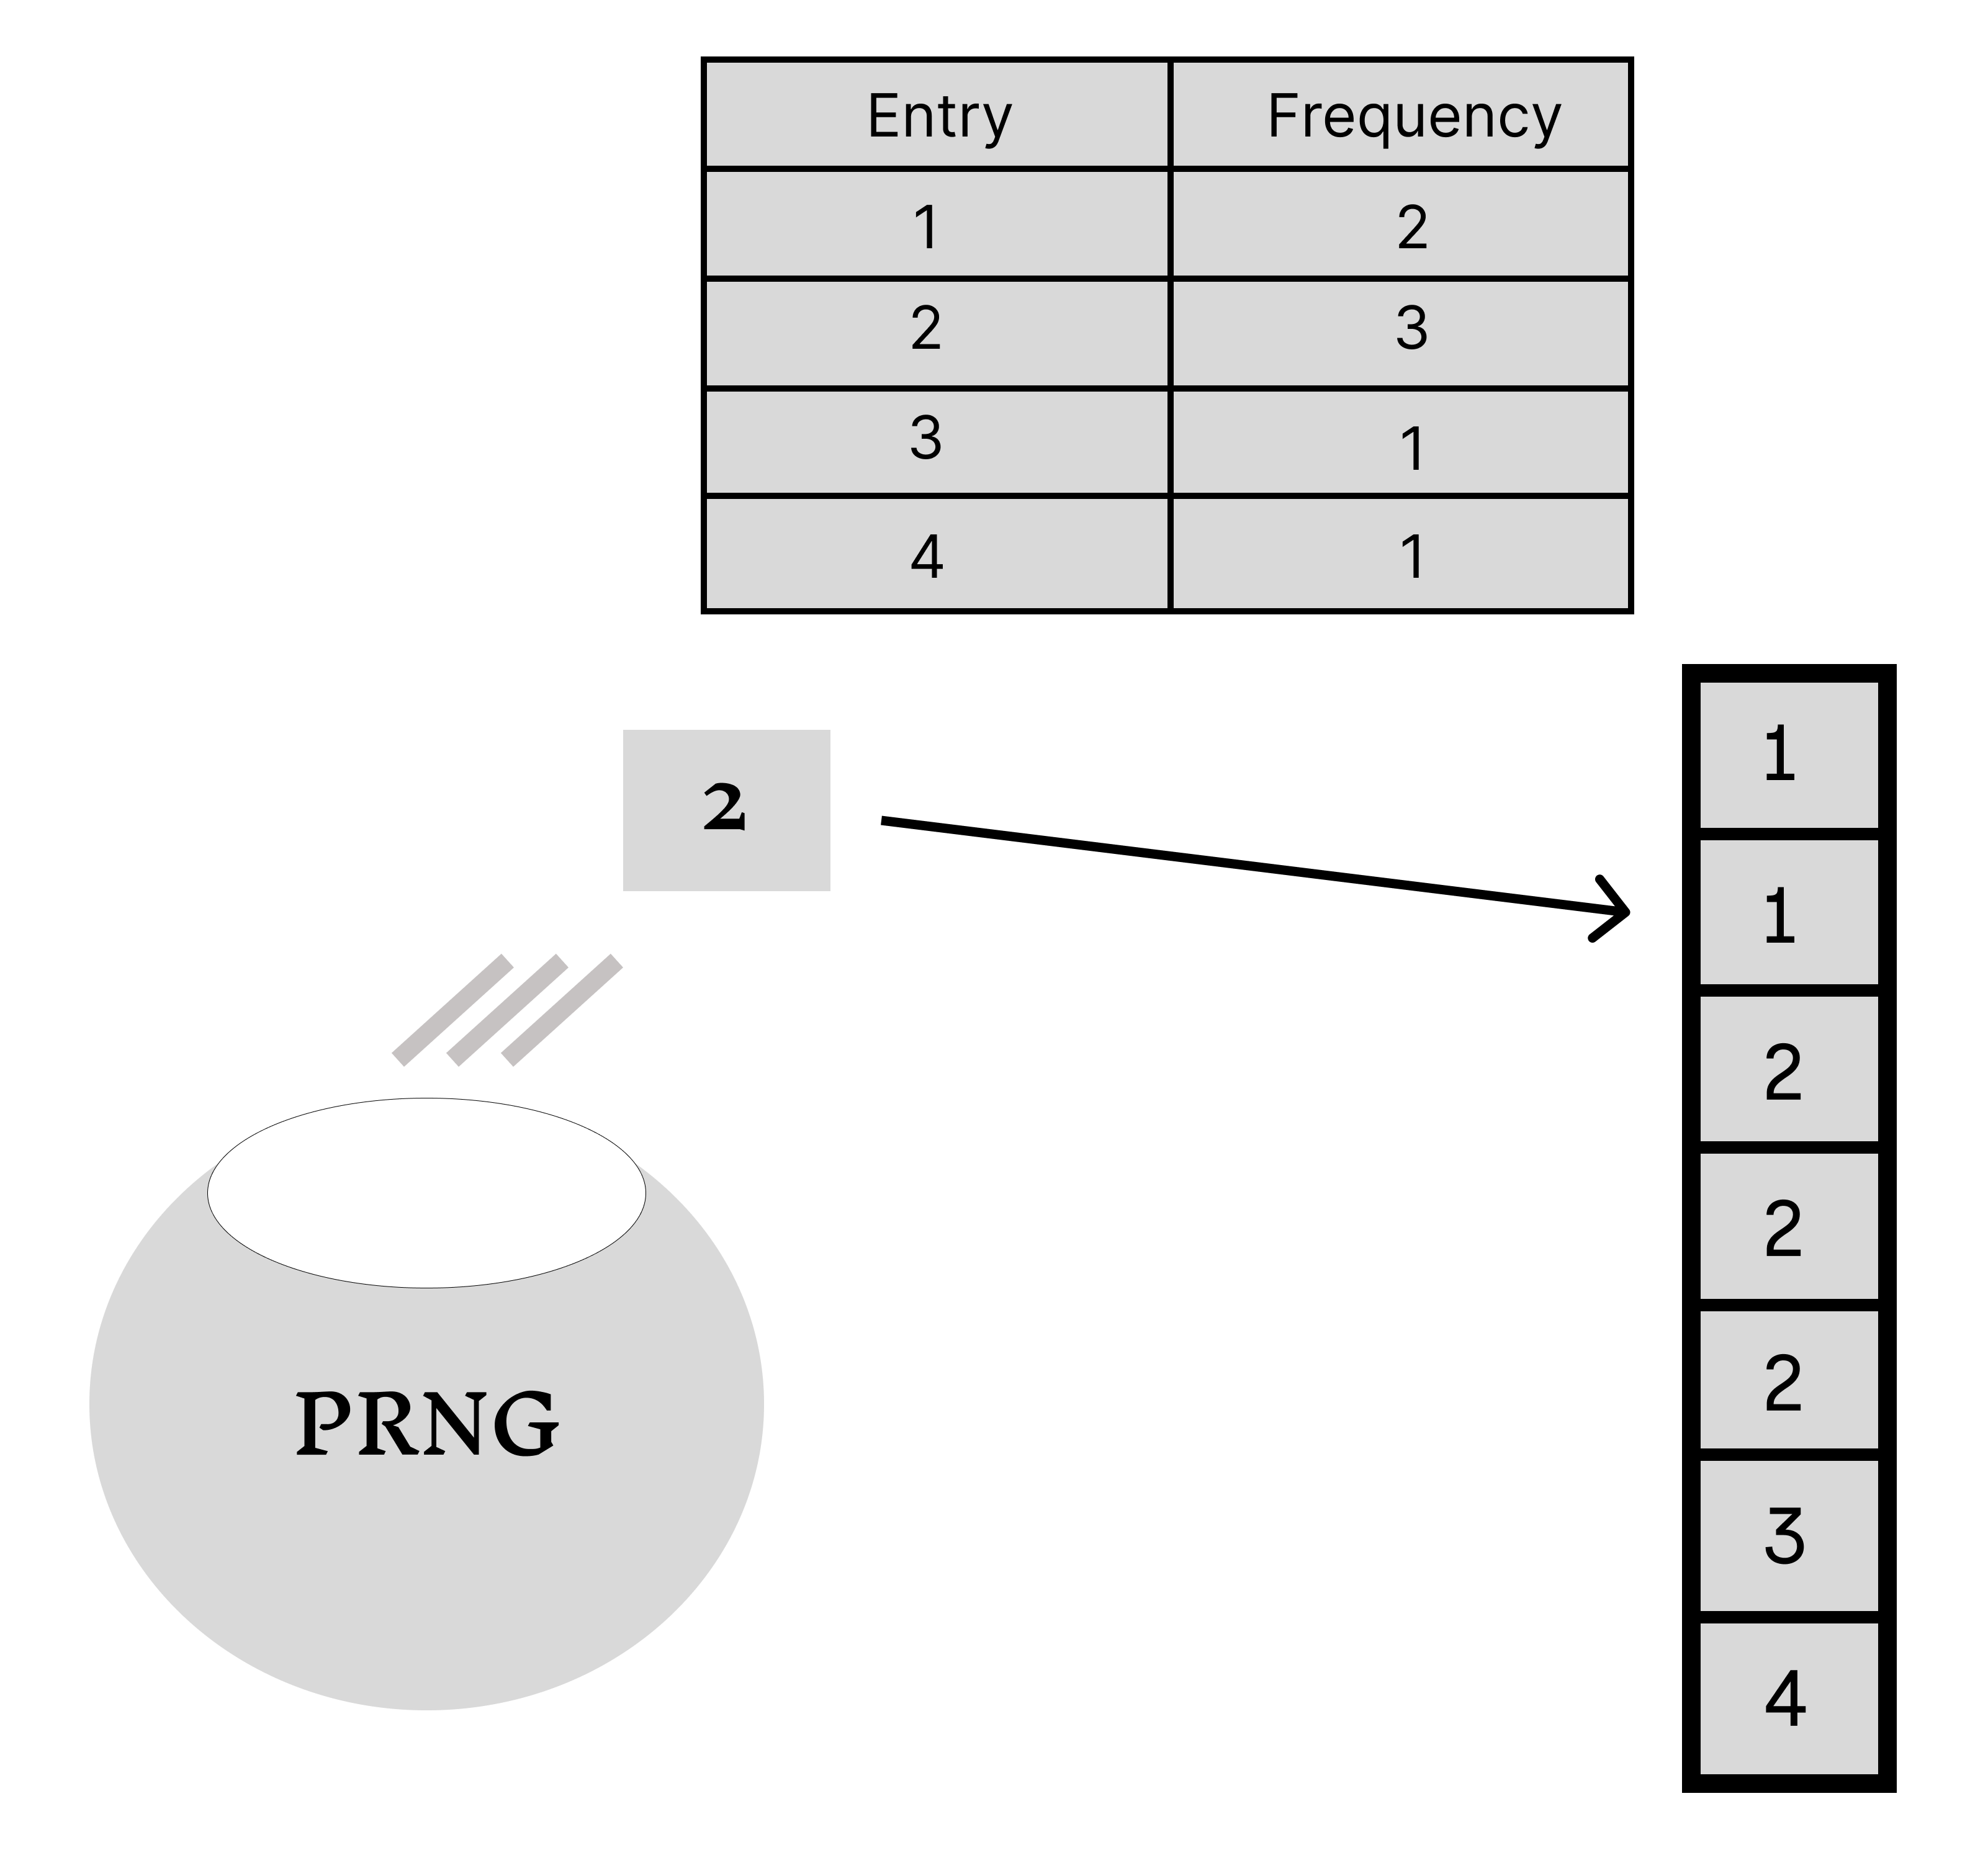
\includegraphics[width=9cm]{figures/marsaglia.png}
    \caption{The table contains the frequency of each index, whereas the array is populated 
    with as many entries as there are occurrences of each index. The sample "2" was generated, which is used to access the second position in the array}
    \label{fig:lookup_table}
\end{figure}

One limitation of this approach is the size of the array being in $O(n)$, which is not feasible for large \textit{support} $N$. 
To circumvent this, Marsaglia and Tsang proposed a \textit{condensed table lookup method} \cite{marsagliaFastGenerationDiscrete2004}, which 
works based on the principle exposed in the table below.

\vspace{0.2cm}
\fbox{
    \parbox{0.83\linewidth}{
        A floating-point number $p$ with $d$ decimal places can be used to represent a probability. For example, assuming $d = 2$, 
        the entry one from the last figure has probability $p(1) = 0.28$. To realize this probability, a table of size $10^2$ is required. 
        In order to achieve reasonable precision, a table of size in the magnitude of $10^{10}$ would be required, which would be unfeasable.
        Alternatively, less space can be used by breaking this table down to $d$ smaller tables. 
        To do this, each probability gets split into $d$ digits $m$, which respectively get $m$ entries in the corresponding table.  Now, generating a uniform integer from the interval $[1,100]$, it is possible to access the correct table and generate the variate.
        \footnotemark
    }
}
\vspace{0.2cm}
\footnotetext{This is a simplified version of the algorithm. For a more detailed explanation, see \cite{marsagliaFastGenerationDiscrete2004}}

\subsection{Approximation Sampling}\label{subsec:jim_gray}
Due to Gray \cite{grayQuicklyGeneratingBillionrecord1994}, this method is a fast approximation of the \textit{Zipfian's} tail and the generalized harmonic number.
The first few probabilities are calculated precisely and normalized by the approximated $H_{N,\alpha}$, while an exponential curve approximates the tail. 
A uniform sample is then used to generate a \textit{Zipfian} variate using inversion.
Figure \ref{fig:jim_gray} makes this idea clear by having two different areas along the x-axis. 

\begin{figure}[h]
    \centering
    \begin{tikzpicture}
    \begin{axis}[
        axis lines=left,
        xmin=0, xmax=30,
        ymin=0, ymax=0.05,
        ytick={0, 0.005, 0.01, 0.03, 0.05},
        yticklabels={0.5\%,1\%, 3\%, 5\%},
        xtick={1, 2, 3, 5, 10, 20, 30, 50},
        height=6cm,
        width=10cm,
        ybar,
        bar width=8pt,
        ymajorgrids=false,
        grid style=dashed,
        ylabel near ticks,
        xlabel near ticks,
        tick label style={font=\small}
    ]

    % Bar plot
    \addplot[ybar, fill=white] coordinates {
        (1, 0.05)
        (2, 0.035)
        (3, 0.025)
        (4, 0.017)
        (5, 0.015)
    };

    % Line plot
    \addplot[smooth, thick] coordinates {
        (5.5, 0.015)
        (10, 0.007)
        (20, 0.003)
        (30, 0.001)
    };

    \end{axis}
\end{tikzpicture}
    \caption{Jim Gray's method for generating samples from a Zipfian distribution}\label{fig:jim_gray}
\end{figure}

The mathematical description of this method is not quite straightforward and is omitted here. For a more detailed explanation, see \cite{grayQuicklyGeneratingBillionrecord1994,knuthArtComputerProgramming1997}.

\paragraph{Summary} As all generation techniques were described, the question remains how to evaluate them for accuracy compared with 
the theoretical probability values yielded by the \ac{PMF} in Equation \ref{eqt:zm_prob} - even for \textit{exact} methods. As these methods are developed, some assumptions
\cite{leydoldErrorDetectionNonUniforma} are taken that might not hold up in the computers used to generate these variates:

\begin{itemize}
    \item There exists a perfectly uniform generator that produces a sequence of \textit{independent} random variables uniformly distributed in $(0,1)$
    \item Computers can save and manipulate real numbers
\end{itemize}

Both of these assumptions cannot be fulfilled. First, the \textit{number generators} used are only pseudo-random \cite{kuhlHistoryRandomVariate2017} and might
have biases and produce correlated subsequences. For the second, computers only have limited precision, and computing terms such as the \textit{generalized harmonic number} suffer from
imprecisions caused by \textit{roundups} and \textit{cutoffs} \cite{leydoldErrorDetectionNonUniforma}. Some distributions such as \textit{power laws} worsen this issue \cite{radicchiUnderestimatingExtremeEvents2014}. Therefore,
we introduce a diverse set of criteria in the following sections for identifying correct implementations and measuring their errors:

\begin{itemize}
    \item Maximal absolute \ac{CDF} difference
    \item Sum of absolute \ac{PMF} differences
\end{itemize}

\section{Error Metrics}
To compare the different methods introduced previously, it is imperative to first define the framework used to evaluate them. Some principles can be applied from the literature
\cite{clausetPowerlawDistributionsEmpirical2009,leydoldErrorDetectionNonUniforma,monahanAccuracyRandomNumber1985}:

\begin{mdframed}
        \begin{enumerate}
            \item Calculate the theoretical distribution for the given parameters: $N$ - support size and $\alpha$ - skew.
            \item Generate an empirical distribution using the algorithms described earlier.
            \item Use a \textbf{goodness-of-fit test} to compare the generated distribution to the theoretical one.
        \end{enumerate}
        \label{box:accuracy}
\end{mdframed}

This framework assumes a "black-box" view of the generating processes and treats the generated samples as a dataset that should be fitted to the theoretical Zipfian. 
At the center of this comparison is a \textbf{goodness-of-fit test}, which tells whether the empirical distribution matches the expected distribution closely enough.
As such, the test requires a \textit{comparison metric} between the two distributions - a function that takes two distributions and returns a number that quantifies their dissimilarity. 
Let us look at the example given in Figure \ref{fig:accuracy-measure}. If the blue curve represents the theoretical distribution and the orange curve is the empirical one,
the shaded area represents the difference between the two. The smaller this area, the better the empirical distribution fits the theoretical one.

\begin{figure}[h]
    \centering
    \begin{tikzpicture}
  \begin{axis}[
    domain=0.5:1.7,
    samples=200,
    width=10cm,
    height=6cm,
    xlabel={$x$},
    ylabel={$f(x)$},
    axis lines=left,
    legend pos=north east,
    clip=false,  % Allows drawing outside the axis box
  ]
    % First distribution: Gaussian-like curve centered at 1.
    \addplot[name path=A, blue, thick] {exp(-((x-1)^2)/(0.02))};
    \addlegendentry{P};
    
    % Second distribution: Similar but slightly shifted right (centered at 1.1).
    \addplot[name path=B, red, thick] {exp(-((x-1.1)^2)/(0.02))};
    \addlegendentry{Q};
    
    % Shade the area between the two curves from x=0.8 to x=1.3.
    \addplot [
      thick,
      color=gray,
      fill=gray,
      fill opacity=0.3
    ] fill between[
      of=A and B,
      soft clip={domain=0.8:1.3},
    ];
    
    % Draw an arrow starting completely right of the graph.
    % It begins at (1.4,0.6) and extends with an offset (1,0.2),
    % with a box in the middle displaying f(P,Q) and an endpoint label "0.8".
    \draw[->, thick] (axis cs:1.4,0.5) -- 
      node[midway, fill=white, draw, rectangle] {$f(P,Q)$} ++(1.0, 0) 
      node[right] {0.8};
      
  \end{axis}
\end{tikzpicture}
    \caption{Accuracy Measure}\label{fig:accuracy-measure}
\end{figure}

For this work, two measures are going to be used: the \textbf{maximal absolute CDF difference}, known in the literature as the \textit{Kolmorgorov-Smirnov} statistic and the 
\textbf{sum of absolute PMF differences}, known in the literature as the \textit{Total Variation distance} \cite{marsagliaEvaluatingKolmogorovsDistribution2003,leydoldErrorDetectionNonUniforma}.
The former is widely used for hypothesis testing and has the advantage of being a non-parametric test, flexible enough for a wide range of distributions \cite{KolmogorovSmirnovTest2008}. It is however
sensitive to outliers. The latter is a more general measure of the difference between two probability distributions and, on the other hand, is more resistant against outliers.

\paragraph{Maximal absolute CDF difference}
This measure is defined as the maximum difference - $D_{n}(P,Q)$ - between the empirical and theoretical
\ac{CDF}. Equation \ref{eq:ks-statistic} formalizes it. It has a nice graphical interpretation as the maximal vertical 
distance between the two \ac{CDF}s, as seen in Figure \ref{fig:ks-test}.

\begin{equation}
D_n = \sup_x |P(x) - Q(x)|
\label{eq:ks-statistic}
\end{equation}

\begin{figure}[h]
    \centering
    \pgfmathdeclarefunction{normalcdf}{1}{%
  \pgfmathparse{1/(1 + exp(-0.07056*(#1)^3 - 1.5976*(#1)))}%
}

\begin{tikzpicture}
    \begin{axis}[
        axis lines = left,
        enlargelimits,
        grid=major,
        domain=-4:4,
        samples=100,
        xlabel=$x$,
        ylabel={CDF},
        legend pos=south east,
        width=10cm,
        height=8cm
    ]

    \addplot [red, thick] {normalcdf(x)};
    \addlegendentry{Target CDF};

    \addplot[
        blue,
        thick,
        const plot,
    ] coordinates {(-4,0)(-3,0)(-2.5,0)(-2,0.02)(-1.5,0.04)(-1,0.08)(-0.5,0.14)(0,0.26)(0.5,0.4)(1,0.54)(1.5,0.64)(2,0.74)(2.5,0.86)(3,0.94)(3.5,0.98)(4,1)};
    \addlegendentry{Empirical CDF};

    \draw[<->, thick] (axis cs:1.5,0.64) -- (axis cs:1.5,{normalcdf(1.5)});
    \node[anchor=east] at (axis cs:1.5,0.76) {$D_{max}(P,Q)$};
    \end{axis}
\end{tikzpicture}
    \caption{Kolmogorov-Smirnov Test}\label{fig:ks-test}
\end{figure}

This measure is then compared to a \textit{standard value} given by a probability function called the 
\textit{Kolmogorov distribution} \cite{marsagliaEvaluatingKolmogorovsDistribution2003}. 

\begin{equation}
    F_n = P[D_n \leq x | \mathcal{H}_0] \quad \text{for} \, x \in [0,1]
    \label{eq:ks-cdf}
\end{equation}

Due to its computational complexity, an exact form of this distribution is prohibitive for bigger \textit{support sizes} $N$.
Consequently, approximations are prefered, such as the one given by Marsaglia \cite{marsagliaEvaluatingKolmogorovsDistribution2003}.
The implementation used in the \textit{SciPy} library follows this work.

% \paragraph{Why the KS distance test is not perfect} Although the theory for the \textit{KS} distance is well developed, it is not completely adequate for
%  very large \textit{sample sizes}, as passing the test becomes increasingly hard. This is due to the growing \textit{test power}, 
%  such that the probability distribution implied in Equation \ref{eq:ks-cdf} approaches 0 with growing sample sizes. 
%  Therefore, the analysis will limit itself to presenting which methods are \textit{more correct} than others 
%  and how \textit{wrong} they are in absolute terms. We now turn to the next distance measure.

\paragraph{Sum of absolute PMF differences}
This distance, also known as \textit{Total Variation Distance (TVD)}, is given by the sum of all absolute differences in the probability mass function of two distributions. More precisely, 
given two (discrete) distributions, $P$ and $Q$, defined in region $X$:

\begin{equation}
    d_{TV}(P,Q) = \frac{1}{2} \sum_{x \in X} |P(x) - Q(x)|    
    \label{eq:total-variation}
\end{equation}

The distance ranges from $0$ to $1$, where zero means the distributions are equal, and $1$ means they are completely different. Interpreting it as a percentage allows statements such as:
"About $y\%$ of the probability mass differs between the theoretical and empirical distribution". Figure \ref{fig:accuracy-measure} was first presented as a general measure,
but is also, in fact, the \textit{TVD}. An important property of the total variation distance is that with growing sample sizes,
the distance between the empirical and theoretical distribution should converge to 0 for 
all $x$ \cite{kengEmpiricalDistributionFunction2016}.
 
As all required notions and metrics are well defined, a detailed description of the research approach comes next. With it, common 
benchmarking tools will be identified in the literature and their popularity evaluated. 
\chapter{Approach}\label{chapter:approach}

\pgfplotstableread[col sep=comma]{data/sys_lit_rev.csv}\mytable

\def\printonlypositive#1{\ifnum#1>0
#1
\fi}

This thesis aims to identify the most widely used frameworks for generating synthetic \textit{Zipfian} distributed data in the systems programming and database community and 
make a comparative evaluation.
The first step required to achieve this is a systematic review of current approaches. The following sections describe
\begin{enumerate}
    \item The \textbf{research approach} used to identify the frameworks
    \item The \textbf{common frameworks} recognized from the search along with short descriptions
    \item The \textbf{popularity and impact} of those tools
    \item The \textbf{benchmarking module} which will be used to evaluate the frameworks
\end{enumerate}

\section{Research Approach}
First, a list of relevant conferences and journals was defined to identify frameworks the systems programming and database community used.
 The six following conferences were taken into account:
\begin{center} 
    \begin{minipage}{0.8\linewidth} 
      \begin{multicols}{2} 
        \begin{itemize}
          \raggedright
          \item \ac{PVLDB}
          \item \ac{SIGMOD}
          \item \ac{CIDR}
          \item \ac{OSDI}
          \item \ac{NSDI}
          \item \ac{FAST}
        \end{itemize}
      \end{multicols}
      \label{list:conferences}
    \end{minipage}
\end{center}

These conferences were chosen due to their high selectivity and special relevancy for storage technology research, where standardized IO benchmarks are prevalent
. The search was conducted broadly following the steps indicated in \parencite{bramerSystematicApproachSearching2018}, as defined below: 
\begin{enumerate}
    \item Word search on keyword search matrix (see table~\ref{tab:keyword_search_matrix})
    \item Identify the frameworks used in the papers
    \item Extended keyword search, this time adding the frameworks identified in the previous step
\end{enumerate} 

The first step suggests the use of a \textit{keyword matrix}. Such a matrix can be built by choosing appropriate keywords
that refer to the topic of interest, so all words should be present in the works searched. 
Synonyms are used to improve the accuracy and scope of the search. It is defined as follows:

\begin{table}[h!]
    \centering
    \begin{tabular}{|c|l|r|r|}
      \hline
       & \multicolumn{1}{c|}{Keyword 1} & \multicolumn{1}{c|}{Keyword 2} & \multicolumn{1}{c|}{Keyword 3} \\ \hline
       \parbox[t]{4mm}{\multirow{3}{*}{\rotatebox[origin=r]{90}{synonyms}}}
       & zipf   &   benchmark     &    synthetic      \\
       & zipfian   &   workload     &    generated      \\
       &    &   evaluation     &    sampled      \\
       &    &   empirical     &    sampler      \\
       &   &   dataset     &         \\ \hline
    \end{tabular}
    \caption{Keyword search matrix}
    \label{tab:keyword_search_matrix}
  \end{table} 

Given this matrix, the search was conducted on the following academic databases: \textit{IEEE Xplore}, \textit{ACM Digital Library}, \textit{DBLP}, and \textit{Google Scholar}. 
The results were sorted in \textit{relevance} order, such that well-cited but also relatively new papers appear at the top. An analysis of the findings follows in the next section.

\section{Common Frameworks}

In the first phase, the following frameworks were identified among the top 20 results of each conference
\begin{center}
    \begin{tabular}{|l|}
        \hline
        \textbf{Frameworks} \\ \hline\hline
        \ac{YCSB} \cite{cooperBenchmarkingCloudServing2010} \\ \hline
        \ac{FIO} \cite{1FioFlexible} \\ \hline
        Sysbench \cite{kopytovAkopytovSysbench2025} \\ \hline
        OLTP-Bench \cite{difallahOLTPBenchExtensibleTestbed2013} \\ \hline
    \end{tabular}
\end{center}

The previous keyword matrix was extended with the frameworks' names to assert their popularity in the six venues. 
Pie charts in Figure \ref{fig:popularity_frameworks} show the trends found.

\begin{figure}[h]
    \centering
    \def\printonlypositive#1{\ifnum#1>0
#1
\fi}

\begin{tikzpicture}

% Pie #1: PVLDB
\begin{scope}[xshift=0cm,yshift=0cm]
  \node[font=\bfseries] at (0,1.8){PVLDB};
  \pie[
    sum=auto,
    radius=1.3,
    text=,
    before number=\printonlypositive,
    color={blue!50!white, red!50!white, green!50!white, orange!50!white}
  ]{
    109/YCSB,
    3/Sysbench,
    3/FIO,
    8/OLTPBench
  }
\end{scope}

% Pie #2: SIGMOD
\begin{scope}[xshift=4cm,yshift=0cm]
  \node[font=\bfseries] at (0,1.8){SIGMOD};
  \pie[
    sum=auto,
    radius=1.3,
    text=,
    before number=\printonlypositive,
    color={blue!50!white, red!50!white, green!50!white, orange!50!white}
  ]{
    18/YCSB,
    2/Sysbench,
    0/FIO,
    2/OLTPBench
  }
\end{scope}

% Pie #3: CIDR
\begin{scope}[xshift=8cm,yshift=0cm]
  \node[font=\bfseries] at (0,1.8){CIDR};
  \pie[
    sum=auto,
    radius=1.3,
    text=,
    before number=\printonlypositive,
    color={blue!50!white, red!50!white, green!50!white, orange!50!white}
  ]{
    4/YCSB,
    0/Sysbench,
    1/FIO,
    1/OLTPBench
  }
\end{scope}

% Pie #4: FAST
\begin{scope}[xshift=0cm,yshift=-4cm]
  \node[font=\bfseries] at (0,1.8){FAST};
  \pie[
    sum=auto,
    radius=1.3,
    text=,
    before number=\printonlypositive,
    color={blue!50!white, red!50!white, green!50!white, orange!50!white}
  ]{
    35/YCSB,
    0/Sysbench,
    3/FIO,
    2/OLTPBench
  }
\end{scope}

% Pie #5: NSDI
\begin{scope}[xshift=4cm,yshift=-4cm]
  \node[font=\bfseries] at (0,1.8){NSDI};
  \pie[
    sum=auto,
    radius=1.3,
    text=,
    before number=\printonlypositive,
    color={blue!50!white, red!50!white, green!50!white, orange!50!white}
  ]{
    24/YCSB,
    0/Sysbench,
    0/FIO,
    0/OLTPBench
  }
\end{scope}

% Pie #6: OSDI
\begin{scope}[xshift=8cm,yshift=-4cm]
  \node[font=\bfseries] at (0,1.8){OSDI};
  \pie[
    sum=auto,
    radius=1.3,
    text=legend,
    before number=\printonlypositive,
    color={blue!50!white, red!50!white, green!50!white, orange!50!white}
  ]{
    26/YCSB,
    0/Sysbench,
    3/FIO,
    0/OLTPBench
  }
\end{scope}

\end{tikzpicture}
    \caption{Popularity of the frameworks in the conferences}
    \label{fig:popularity_frameworks}
\end{figure}

The most popular framework is \textbf{YCSB}, followed by \textbf{OLTPBench}, as well as \textbf{FIO}. Although this would point to a clear winner in \textbf{YCSB}, 
it is important to note that the popularity of a framework considered in academic journals might not reflect its actual usage in practice. 
A search for the frameworks in \textit{GitHub} yielded the table \ref{fig:popularity_frameworks} (as of 22 March 2025), containing
the number of \textit{starts} given to a code repository. 

\begin{table}[h]
    \centering
    \begin{tabular}{|l|r|}
      \hline
      \textbf{Framework} & \textbf{Stars} \\ \hline\hline
      YCSB & 5k \\ \hline
      Sysbench & 6.3k \\ \hline
      FIO & 5.5k \\ \hline
      OLTPBench & 0.5k \\ \hline
    \end{tabular}
    \caption{Popularity of the frameworks on GitHub}
    \label{tab:popularity_github}
\end{table}

\subsection{Yahoo! Cloud Serving Benchmark}
\ac{YCSB} is a widely used benchmarking tool for cloud databases, developed by \textit{Yahoo! Research} and now maintained by a community of developers. 
The framework generates \textit{workloads} used to test the performance of database systems under stress, by populating tables with entries. How these entries are distributed
is not fixed and can be chosen by the user. One of the possible distributions is the \textit{Zipfian}, and a submodule in \ac{YCSB} is responsible for generating variates.

In order to compute the samples, the benchmark suite uses the algorithm proposed by Gray, as presented before (see \ref{subsec:jim_gray}). One limiting factor in his original paper
 is that generated keys are lexicographically sorted, e.g. key $0$ has the highest frequency. 
 The keys should be randomly distributed within the support distribution to better reflect real workloads.
See Figure \ref{fig:zipfian_comparison_ycsb} for a comparison of these two cases.

% TODO : Fix x,y-axis labels 
\begin{figure}[h]
    \centering
    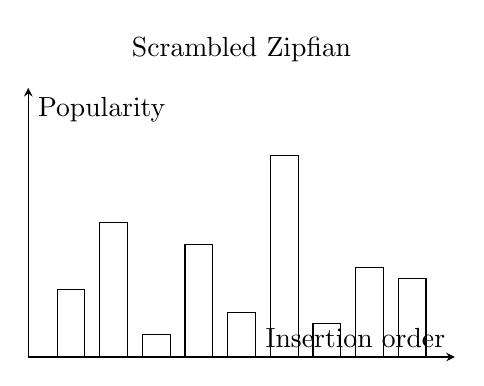
\begin{tikzpicture}
        \begin{axis}[
            width=7cm,
            height=5cm,
            title={Scrambled Zipfian},
            xlabel style={at={(axis description cs:0.5,-0.1)},anchor=north},
            ylabel style={at={(axis description cs:-0.1,.5)},rotate=90,anchor=south},
            xlabel={Insertion order},
            ylabel={Popularity},
            xtick=\empty,
            ytick=\empty,
            axis lines=middle,
            ymin=0, ymax=1.2,
            xmin=0, xmax=10
        ]
        \addplot[ybar,fill=white,draw=black] coordinates {(1,0.3) (2,0.6) (3,0.1) (4,0.5) (5,0.2) (6,0.9) (7,0.15) (8,0.4) (9,0.35)};
        \end{axis}
    \end{tikzpicture}
    \hspace{1cm}
    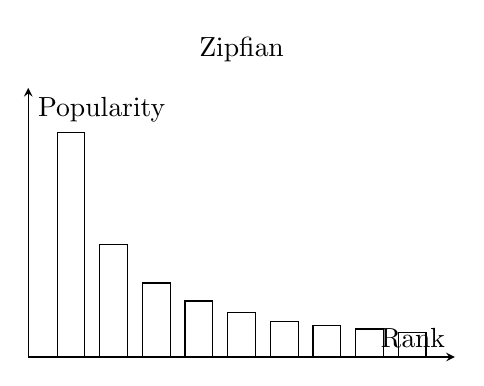
\begin{tikzpicture}
        \begin{axis}[
            width=7cm,
            height=5cm,
            title={Zipfian},
            xlabel style={at={(axis description cs:0.5,-0.1)},anchor=north},
            ylabel style={at={(axis description cs:-0.1,.5)},rotate=90,anchor=south},
            xlabel={Rank},
            ylabel={Popularity},
            xtick=\empty,
            ytick=\empty,
            axis lines=middle,
            ymin=0, ymax=1.2,
            xmin=0, xmax=10
        ]
        \addplot[ybar,fill=white,draw=black] coordinates {(1,1) (2,0.5) (3,0.33) (4,0.25) (5,0.2) (6,0.16) (7,0.14) (8,0.125) (9,0.11)};
        \end{axis}
    \end{tikzpicture}
    \caption{Comparison of Jim Gray's version (right) and the one employed by YCSB (left).}
    \label{fig:zipfian_comparison_ycsb}
\end{figure}

To avoid the issue described earlier, YCSB uses a hashing function to randomly spread the values in support of the distribution and employs an extended domain to reduce collisions \cite{cooperBenchmarkingCloudServing2010}. 

\begin{figure}[h]
  \centering
  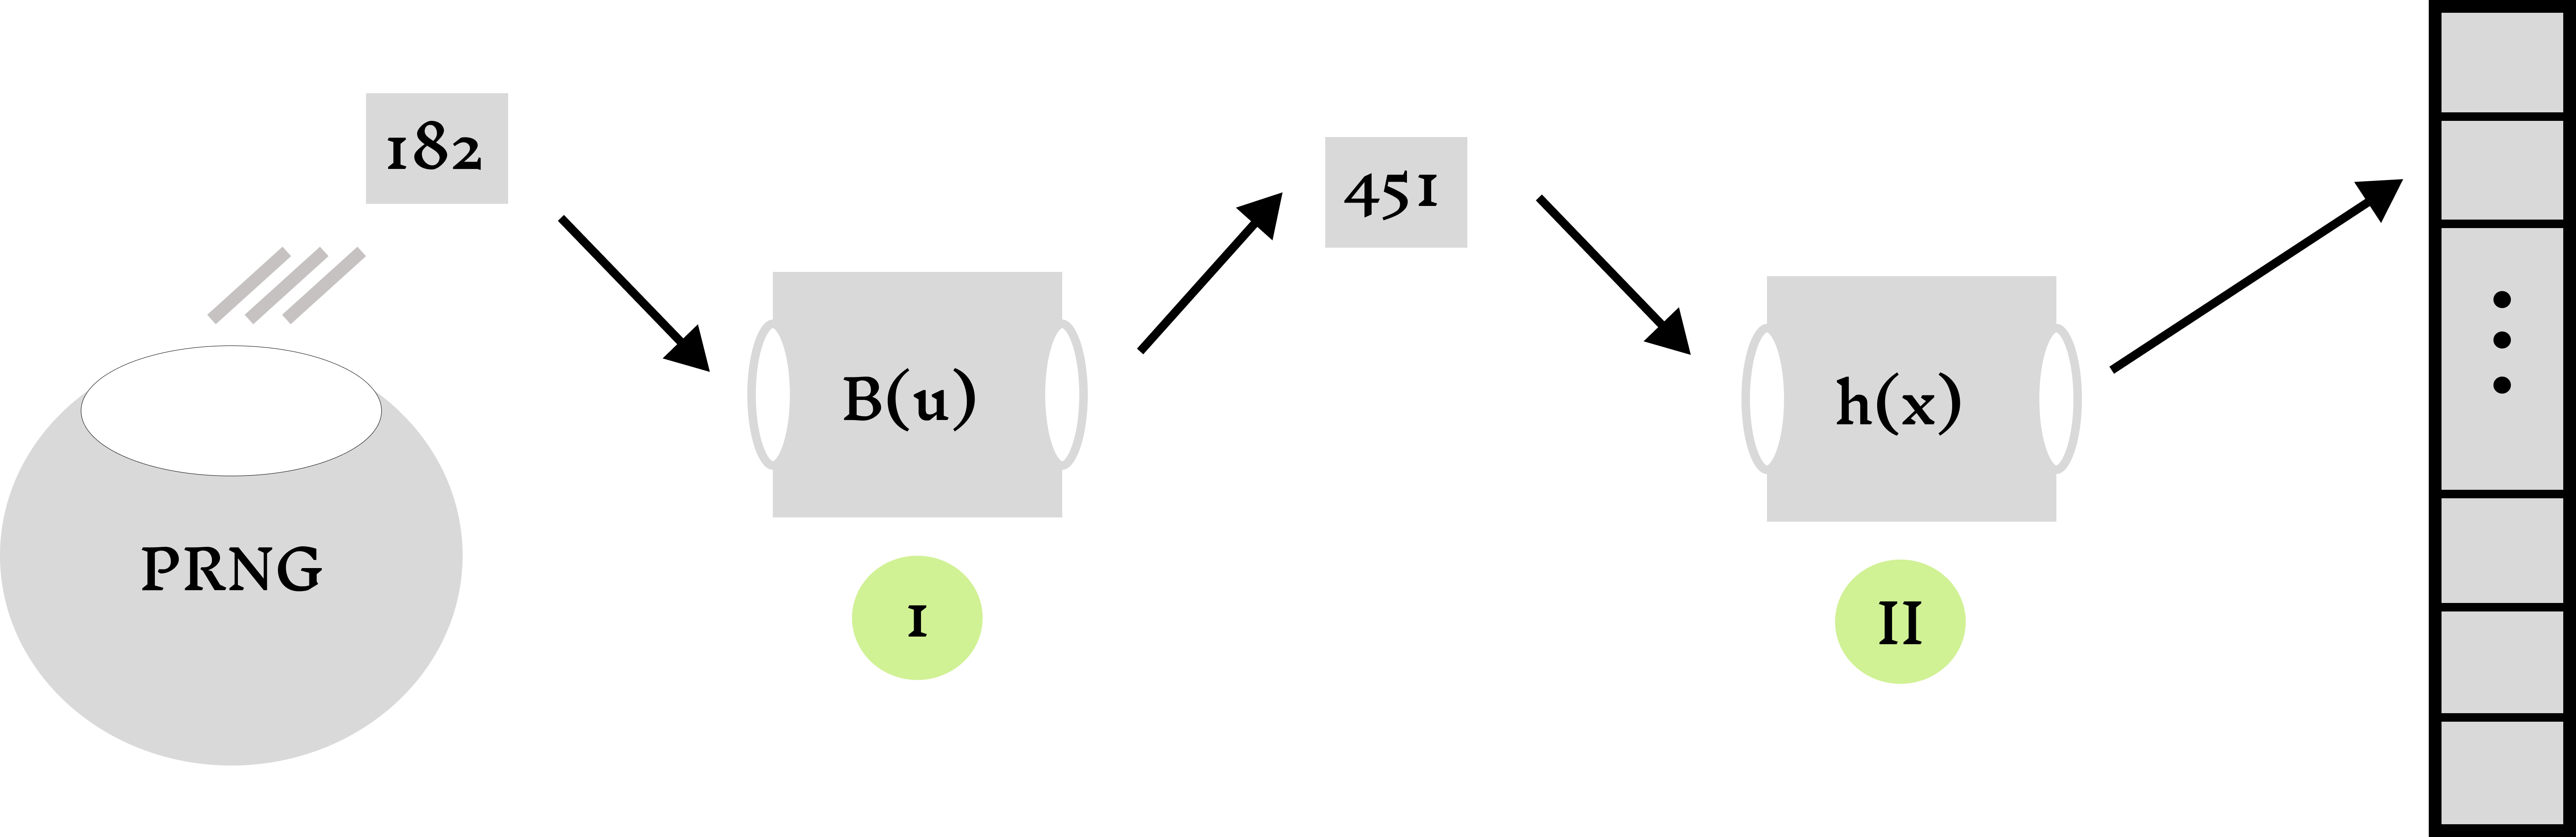
\includegraphics[width=\linewidth]{figures/explanation_ycsb.png}
  \caption{YCSB does sampling by inversion (1) and then hashes the value to spread in in the available range (2)}
  \label{fig:explanation_rej_samp}
\end{figure}

\subsection{Flexible I/O Tester (FIO)}
\ac{FIO} \cite{1FioFlexible} is a benchmarking tool for storage systems. Much like YCSB, its purpose is generating workloads following a certain \textit{access pattern}
to test a storage system. The workloads can vary in type, including sequential or random, and read-only, write-only, or mixed. In the case of \textbf{random I/O}, the user can
change the workload to simulate both asymmetrical and more symmetrical workloads. The underlying distributions include the \textit{Zipfian}, \textit{Normal},
 \textit{Pareto}, and \textit{Uniform} distributions.
 
The algorithm used is also the approximative method due to Jim Gray. As with \ac{YCSB}, the same problem arises with the lexographical ordering of the results, to which
\textit{FIO} resorts to using a hashing function called \textit{lookup3}, in the \textit{Jenkins} collection of hash functions \cite{jenkinsLookup3}.

\subsection{Sysbench}
Sysbench is a benchmarking tool for databases as well as storage systems. It works 
very similarly to YCSB, using multi-threading to strain the system with concurrent accesses. The tool can generate synthetic data
according to different probability distributions, among which the Zipfian distribution.

What sets it apart from the previous is that the variate generation uses a different algorithm. The one employed by Sysbench is based on \textit{Rejection-Inversion sampling} (see Subsection \ref{subsec:rejection_inversion}), 
and the implementation closely follows that from the Apache Commons Math library \cite{MathCommonsMath} under \textit{RejectionInversionZipfSampler}.

\subsection{OLTP-Bench}
The OLTP-Bench \cite{difallahOLTPBenchExtensibleTestbed2013} strives to unify different benchmarks for evaluating a \ac{DBMS}. 
It favors a modular design, enabling very different benchmarks
to be used under a standard interface, which makes it extensible. However, it also has enough benchmarks built-in to be used directly, 
including AuctionMark \cite{AuctionMarkOLTPBenchmark}, \ac{TPC-C}, and \ac{YCSB}. The focus will be on the AuctionMark benchmark,
as it is the one excepting \ac{YCSB}, which generates synthetic data following a Zipfian distribution. The implementation is almost directly based on YCSB, thus not
further differentiated.

\section{Benchmarking Module}
A benchmarking module was developed to evaluate the frameworks. It was written in Python and
allows the user to specify which sample generator to use, as well as the distribution parameters. It is usable from the command line and
includes the following commands: \verb|sample_zipf|, to generate a Zipfian distribution, \verb|accuracy_zipf| to calculate accuracy measures
for one distribution, and \verb|benchmark| to run a specified performance benchmark. It follows a modular design, with the following interfaces:
\textit{SamplerInterface}, responsible for providing a common wrapper interface to all the sampling algorithms; \textit{StorageInterface}, which defines how the 
data is to be stored in memory before processing; and \textit{OutputInterface}, which defines how the data is to be persisted. A UML diagram of the tool is shown in Figure \ref{fig:uml_diagram}.
\begin{figure}
  \centering
  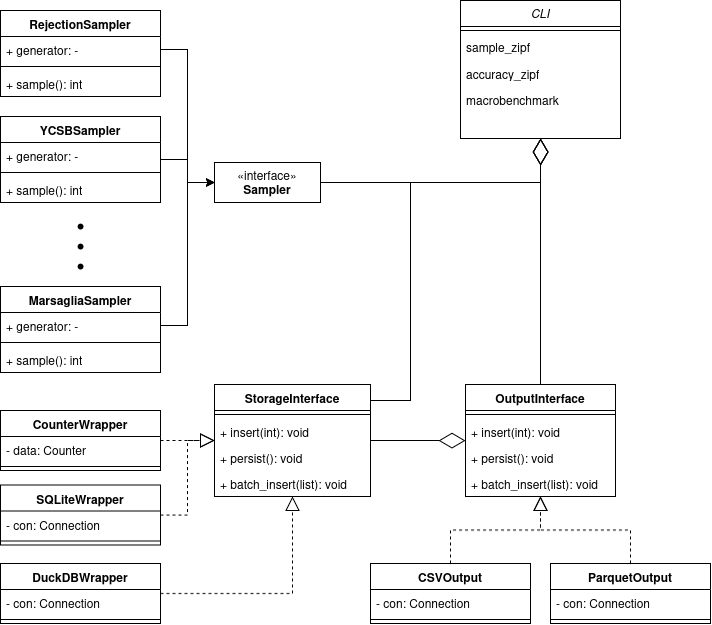
\includegraphics[scale=0.5]{figures/UML.png}
  \caption{UML diagram of the benchmarking module}
  \label{fig:uml_diagram}
\end{figure}

To use the libraries and frameworks described previously, only the necessary code functionality for generating \textit{Zipfian} variates was extracted and packaged
as \textit{shared libraries} and/or \textit{executables}. These were compiled with optimization turned on to ensure a fair comparison.

\subsection{Commands}
To generate a sample, the command \verb|sample_zipf| is used. For example,
\begin{lstlisting}
  sample_zipf --generator sysbench --n 1000 --samples 1000 --skew 1.5 --output csv --storage sqlite --buckets 100
\end{lstlisting}

Running the command will create a CSV file with 1000 samples following a Zipfian distribution with a skew of $1.5$ and a domain from 0 to 1000.
The samples will be stored in memory in a SQLite database with 100 buckets. 

In order to calculate the accuracy measures of the distribution implied by a sample stored in a CSV, the command \verb|accuracy_zipf| is used, as in
\begin{lstlisting}
  accuracy_zipf --input_dir /path/to/csv --skew 1.5 --output_dir /path/to/output
\end{lstlisting}

This method assumes that the directory contains CSV files of results of various sample sizes and domain sizes, belonging to one generator. 
It will then generate 3 CSV files, with columns for domain size and rows for domain sizes - The first one with the \ac{TVD},
the second with the \ac{KS} distance, and the third with the p-value of the \ac{KS} test.

\newtcolorbox{perfbox}[2][]{enhanced,
    boxrule=0.5pt,
    colframe=black,
    colback=white,
    sharp corners,
    fonttitle=\bfseries,
    attach boxed title to top left={xshift=2mm,yshift*=-\tcboxedtitleheight/2},
    boxed title style={
        size=small,
        colframe=black,
        colback=black,
        sharp corners,
        boxrule=0.5pt
    },
    title=#2,#1
}

\chapter{Evaluation}\label{chapter:evaluation}

In the previous chapters, some variate generators included in common frameworks were briefly presented, as well as the underlying 
algorithms used to sampled the Zipfian distribution. To make a fair comparison, it's necessary to evaluate the accuracy of the distributions generated, 
as well as the performance of the algorithms used to generate them. Additionally, simplicity of the methods will be considered. 

\begin{itemize}
    \item \textbf{Accuracy}: The statistical properties of the generated distributions will be compared to the expected values given by the theoretical Zipfian distribution
    \item \textbf{Performance}: The time taken to generate the distributions will be measured and compared using standard profilling tools as well as custom-written benchmarks
\end{itemize}

The variate generators considered for this approach are exactly those presented in the previous chapters: \ac{YCSB}, \ac{FIO}, Sysbench and OLTP-Bench (which will be aliased by Rejection-Inversion - Java), along with
implementations of the algorithms discussed in \ref{chapter:approach}: Rejection and Condensed Table Lookup. Rejection-Inversion wasn't separately implemented since Sysbench already does it.

\section{Experimental Setup}

This section describes the hardware and software environment used to conduct the experiments. All experiments described in this chapter were conducted on a machine with the specifications detailed in table \ref{tab:computer-specs}.
The software environment used is detailed in table \ref{tab:software-environment}.
Since the samplers were implemented in different languages, it's also necessary to detail the versions of the interpreters used to run them (see \ref{tab:interpreter-versions}).

\begin{table}[t]
    \centering
    \begin{tabularx}{\linewidth}{>{\raggedright\arraybackslash}X >{\raggedright\arraybackslash}X >{\raggedright\arraybackslash}X >{\raggedright\arraybackslash}X >{\raggedright\arraybackslash}X}
        \hline
        \textbf{CPU Model} & \textbf{Clockspeed} & \textbf{Number of Cores} & \textbf{Memory Capacity} & \textbf{Memory Speed} \\
        \hline
        AMD Ryzen 7 5850U & 3.6 GHz & 8 & 16 GB & 3200 MHz \\
        \hline
    \end{tabularx}
    \caption{Computer Specifications}\label{tab:computer-specs}
\end{table}

\begin{table}[t]
    \centering
    \begin{tabularx}{\linewidth}{X X X X}
        \hline
        \textbf{Operating System} & \textbf{Kernel Version} & \textbf{Relevant Tools} \\
        \hline
        Debian GNU/Linux 12 & 6.1.0-amd64 & perf\cite{PerfLinuxProfilinga}, JMH \cite{AvoidingBenchmarkingPitfalls}, Google Benchmark \cite{GoogleBenchmarkMicrobenchmark}\\ 
    \end{tabularx}
    \caption{Software Specification}\label{tab:software-environment}
\end{table}


\begin{table}[ht!]
    \centering
    \begin{tabularx}{\linewidth}{>{\raggedright\arraybackslash}X >{\raggedright\arraybackslash}X >{\raggedright\arraybackslash}X}
        \hline
        \textbf{Language/Version} & \textbf{Compiler} &\textbf{Benchmark/Sampler} \\
        \hline
        C++20 & gcc 12.2.0 & Own implementation\\
        \hline
        Java 17 & OpenJDK 17.0.8 & YCSB \\
        \hline
        C (GNU17) & gcc 12.2.0 & Sysbench, FIO \\
        \hline
        Rust & 1.58.0 & None \\
    \end{tabularx}
    \caption{Interpreter Versions}\label{tab:interpreter-versions}
\end{table}

\section{Methodology}
Evaluations were conducted both for accuracy and performance. 
\paragraph{Accuracy} To measure accuracy 2 quantifiable criteria will be used
to offer well-rounded view of the quality of the generated distributions - the \textbf{Kolmogorov-Smirnov test} and the \textbf{Total Variation Distance} as explained
previously in \ref{chapter:background}. All of these are well explored in the literature \cite{clausetPowerlawDistributionsEmpirical2009,leydoldErrorDetectionNonUniforma,dengRobustnessNonuniformRandom1992,monahanAccuracyRandomNumber1985}. 

Besides these numerical quantities, a qualitative approach will be also taken to ensure the measures can be well interpreted. To this end, two visual techniques will also be
used: a \textbf{log-scaled graph} (see \ref{fig:loglog_zipf}) and a \textbf{frequency ratio analysis}. These help identify systematic deviations as well as deviations correlated 
with the rank of the indexes. Table \ref{tab:criteria} gives an overview of the criteria used for the evaluation and how each simulation was run.

\begin{table}[h]
    \centering
    \begin{tabular}{|l|l|l|l|}
        \hline
        \textbf{Criteria} & \textbf{Support Size} & \textbf{Skew} & \textbf{Number of Samples} \\
        \hline
        Log-scaled graph & $10^6$ & 0.8 & $10^9$ \\
        \hline
        Frequency Ratio Analysis & $10^6$ & 0.8 & $10^9$ \\
        \hline
        Kolmogorov-Smirnov Test & $10^8$ & 0.8 & $10^4$ to $10^9$ \\
        \hline
        Total Variation Distance & $10^8$ & 0.8 & $10^4$ to $10^9$ \\
        \hline
    \end{tabular}
    \caption{Simulation specification for each accuracy criteria}\label{tab:criteria}
\end{table}


\paragraph{Performance} The main measure of interest is \textit{throughput} - the amount of variates generated in a time interval (e.g. $10M/ms$). Since benchmarking in modern systems is a rife with
pitfalls \cite{AvoidingBenchmarkingPitfalls,beyerBenchmarkingResourceMeasurement2015}, some precautions should be taken before running the code. More details follow in the coming sections.

\section{Evaluating accuracy}
To first identify which distributions are very wrong, a simple visual inspection is done of the graphs in Figure \ref{fig:pmf-graphs}.  The only distributions which visibly deviate from the expected curve are the FIO and the Condensed Table Lookup. These will be investigated later on. 

\begin{figure}[H]
    % First row
    \centering
    \begin{subfigure}{0.46\textwidth}
        \centering
        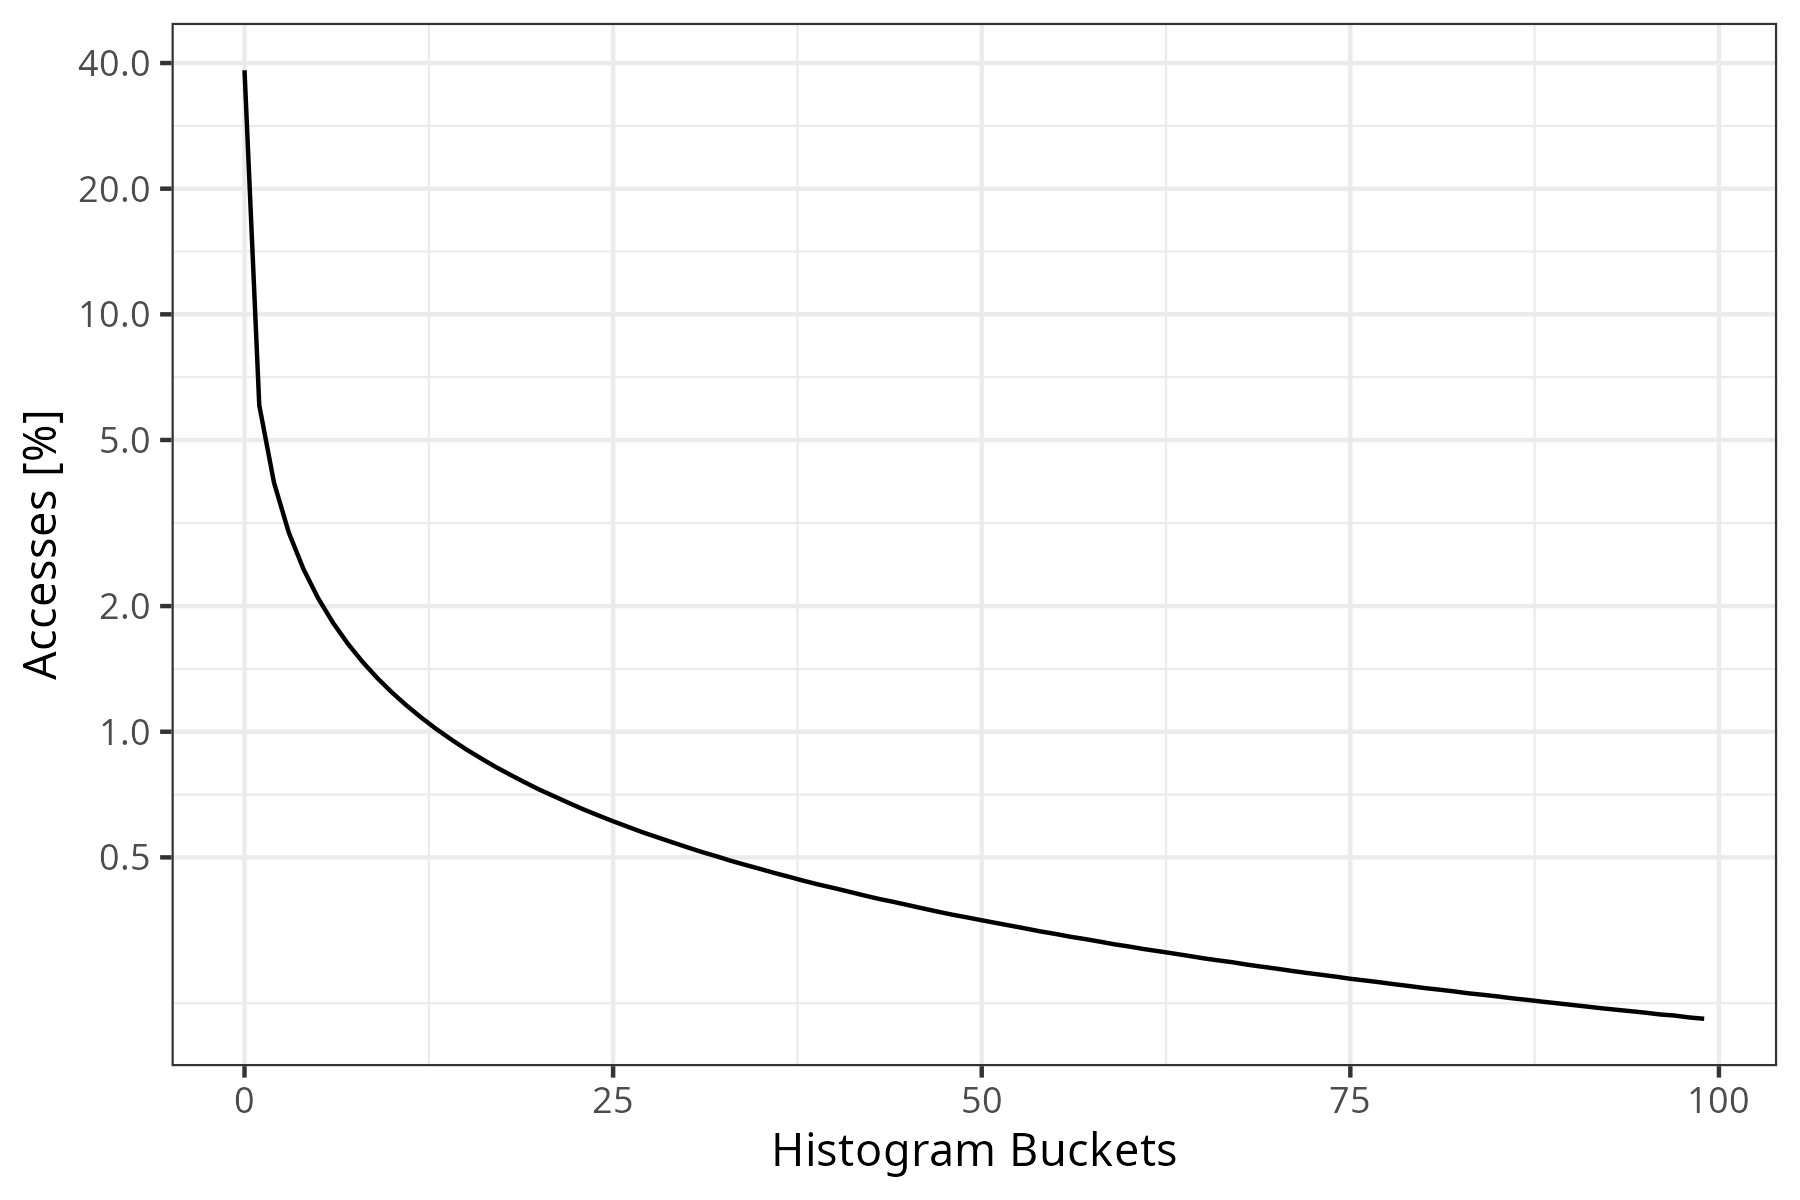
\includegraphics[width=\textwidth]{figures/pmf/apache.png}
        \caption{Rejection inversion}
    \end{subfigure}
    \hfill
    \begin{subfigure}{0.46\textwidth}
        \centering
        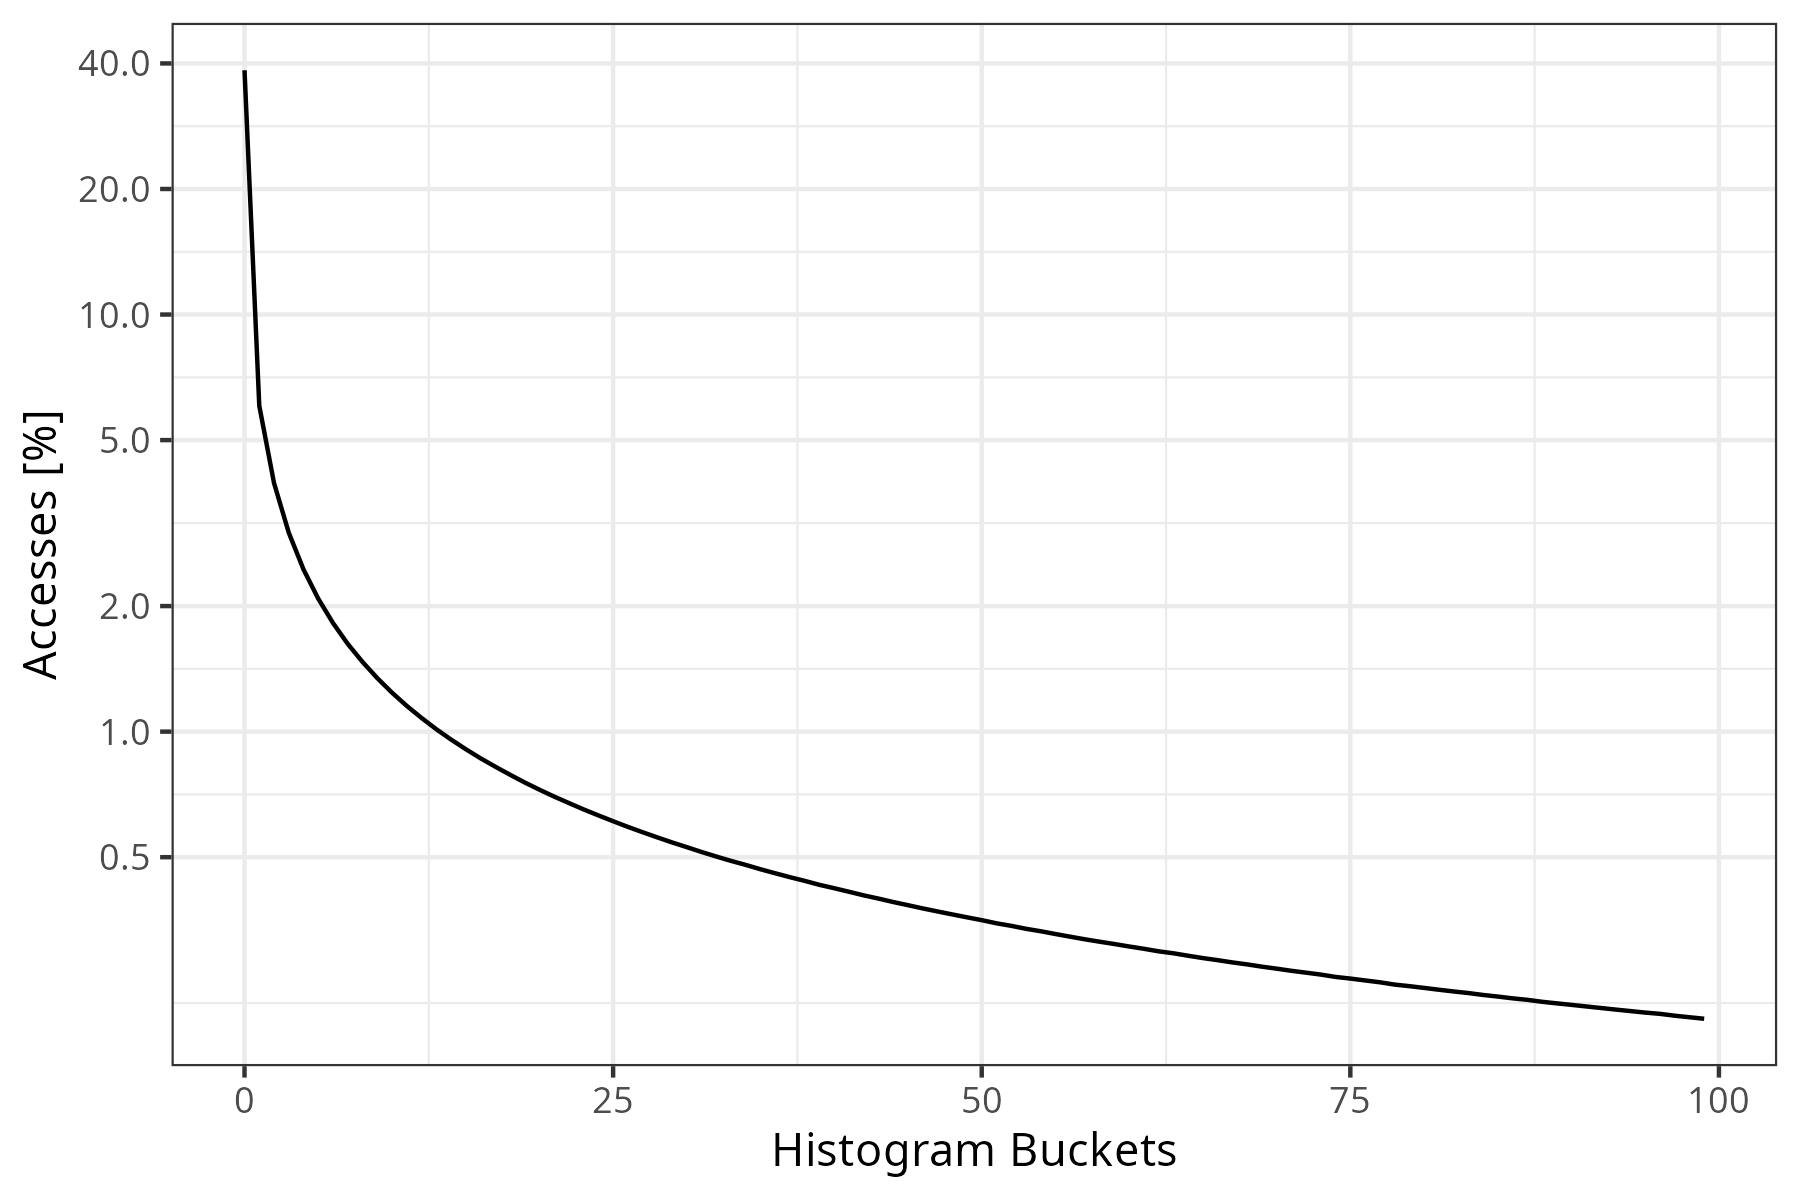
\includegraphics[width=\textwidth]{figures/pmf/ycsb.png}
        \caption{YCSB}
    \end{subfigure}
    \\ 
    % Second row
    \begin{subfigure}{0.46\textwidth}
        \centering
        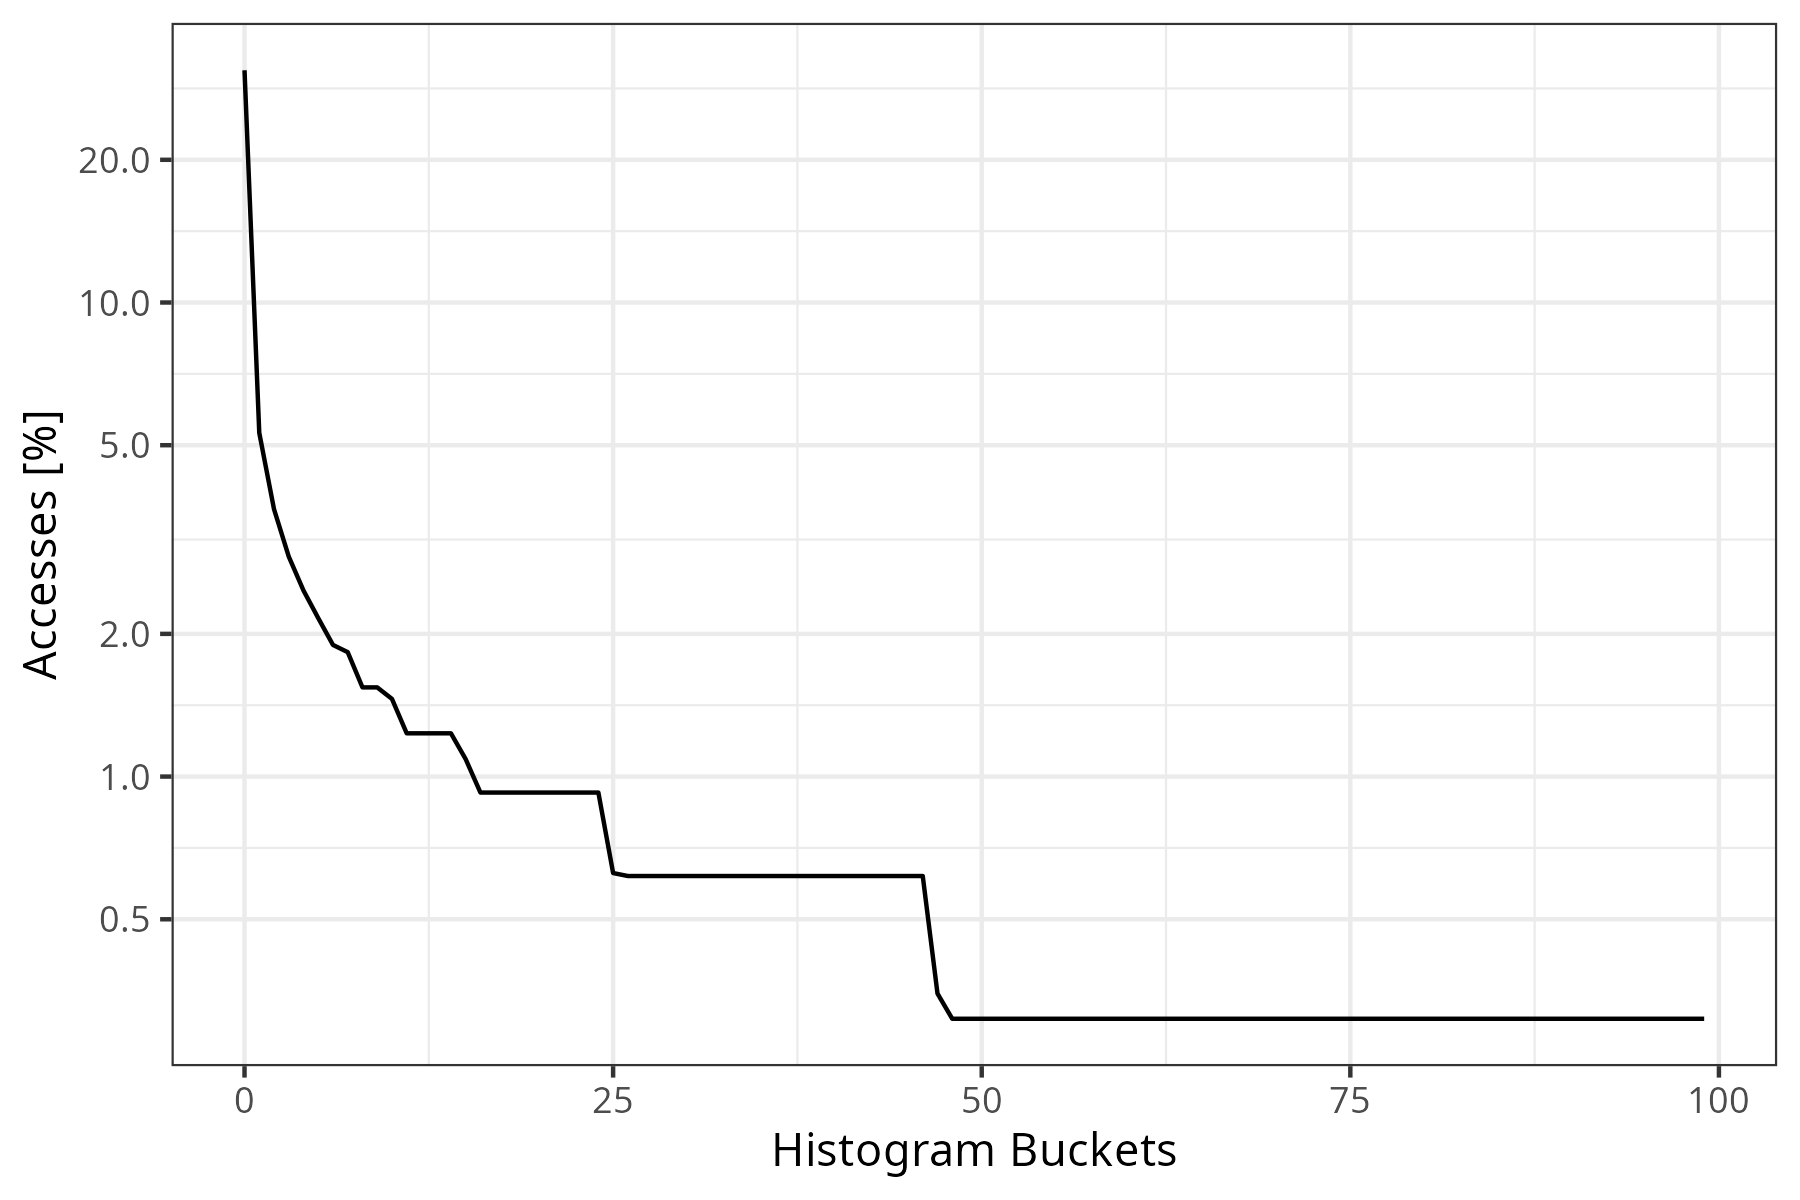
\includegraphics[width=\textwidth]{figures/pmf/fio.png}
        \caption{FIO}
    \end{subfigure}
    \hfill
    \begin{subfigure}{0.46\textwidth}
        \centering
        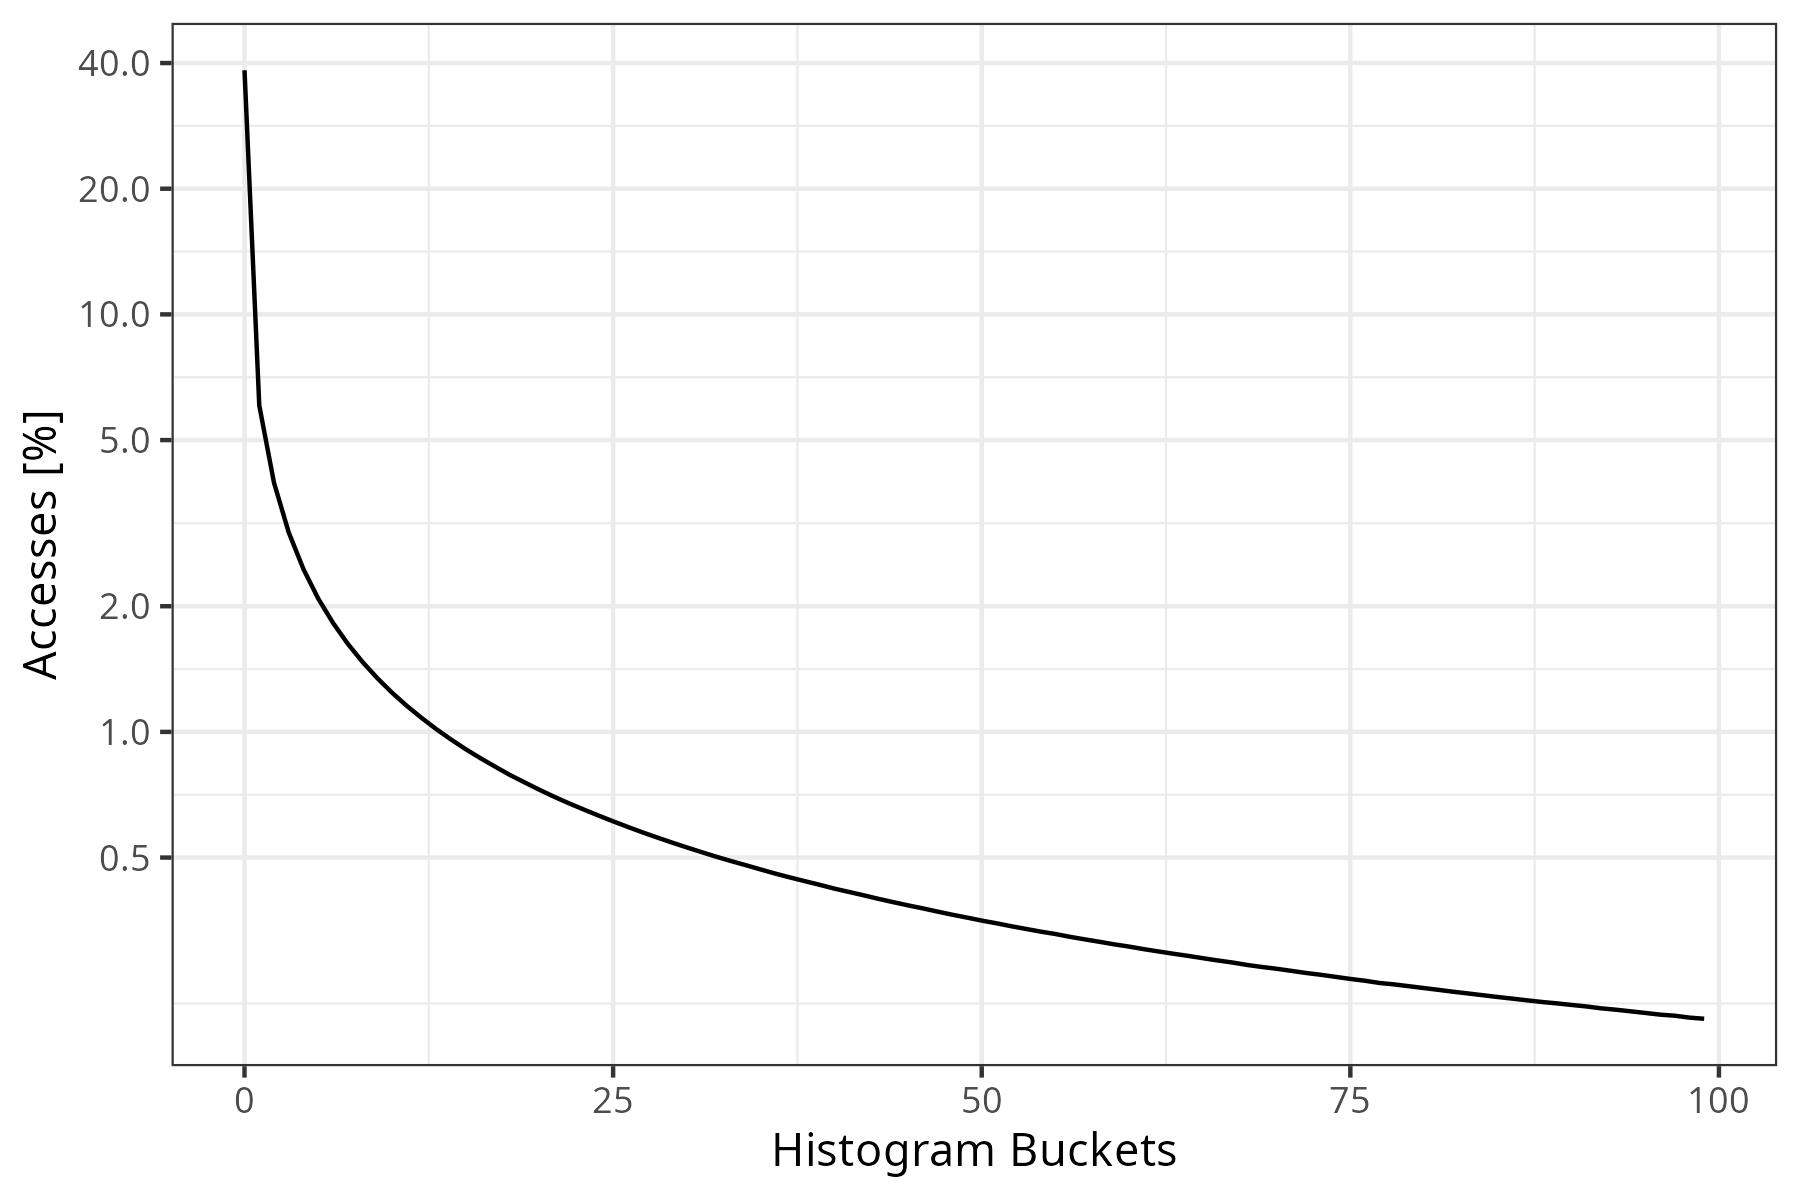
\includegraphics[width=\textwidth]{figures/pmf/sysbench.png}
        \caption{Sysbench}
    \end{subfigure}
    \\    
    % Third row
    \begin{subfigure}{0.46\textwidth}
        \centering
        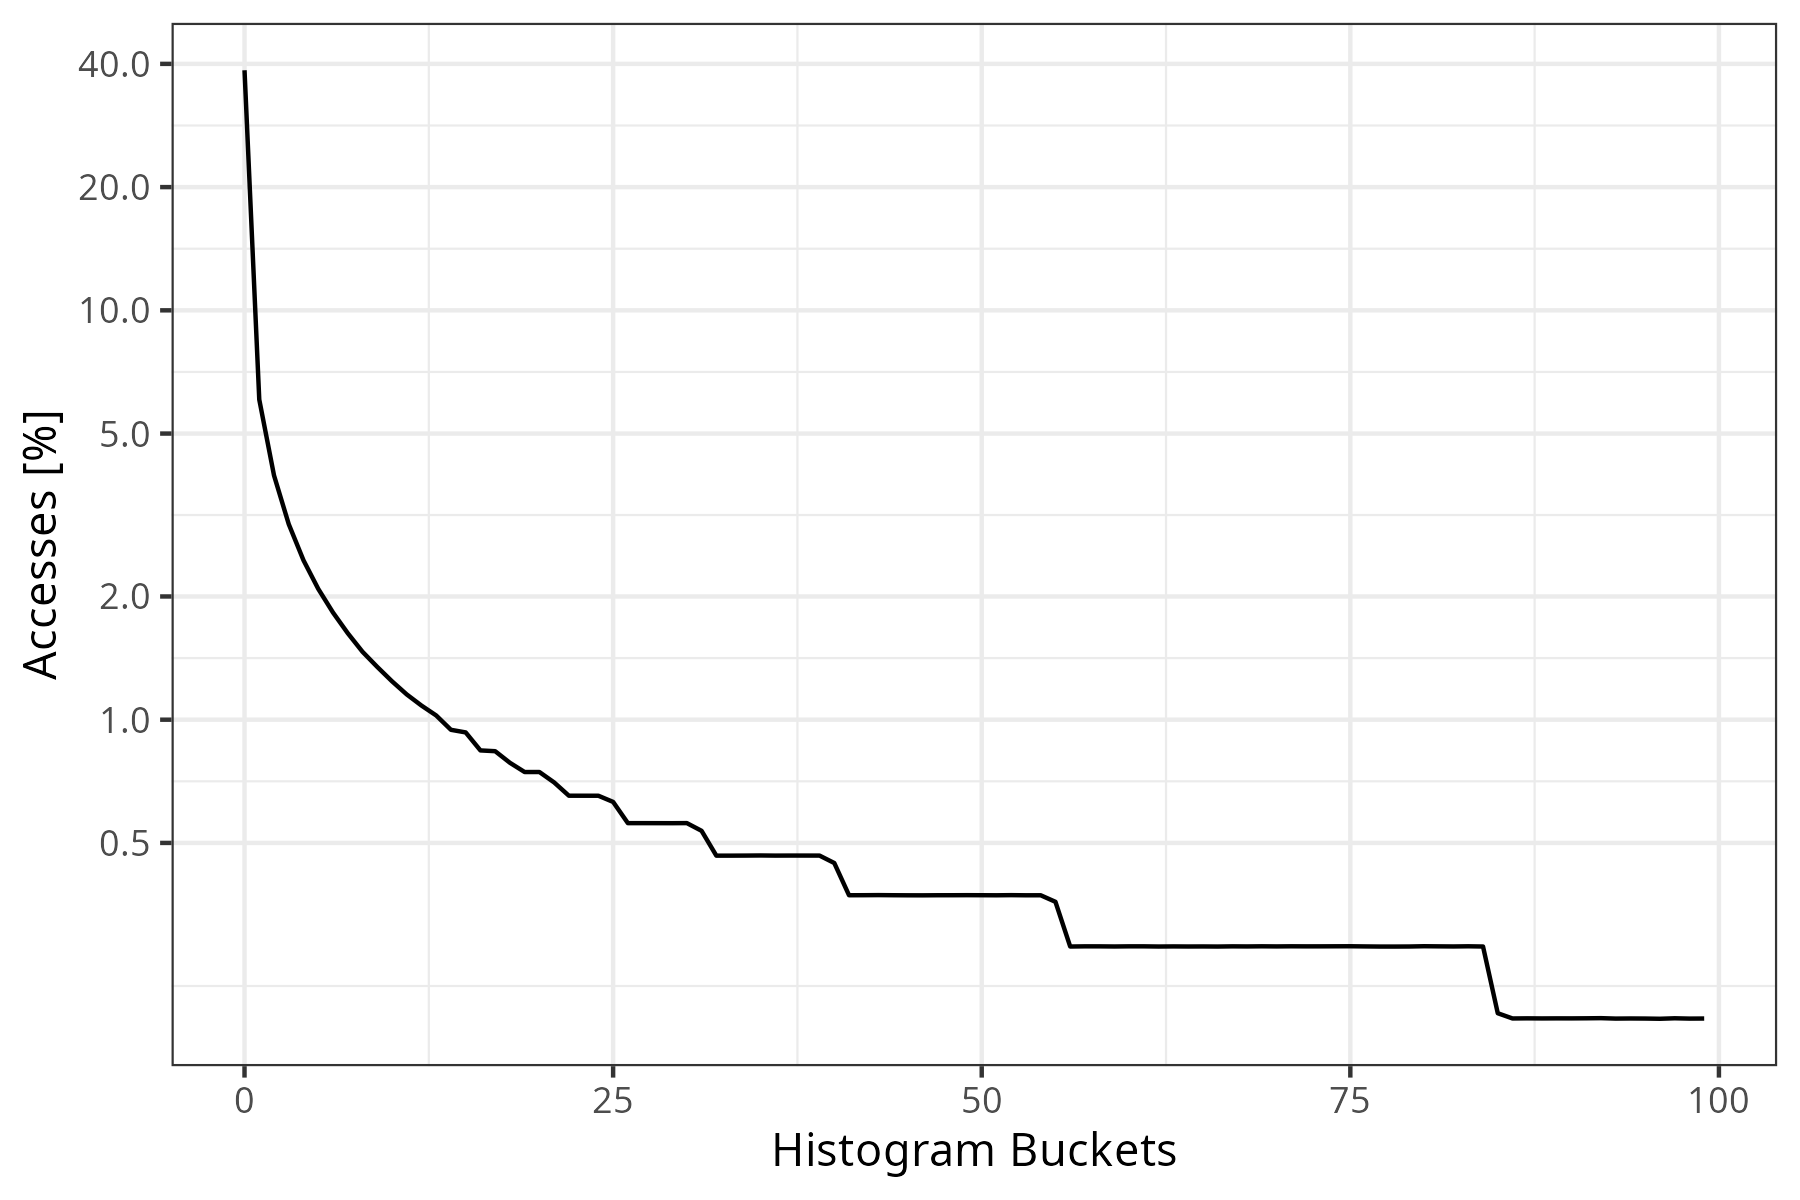
\includegraphics[width=\textwidth]{figures/pmf/marsaglia.png}
        \caption{Condensed Table Lookup}
    \end{subfigure}
    \hfill
    \begin{subfigure}{0.46\textwidth}
        \centering
        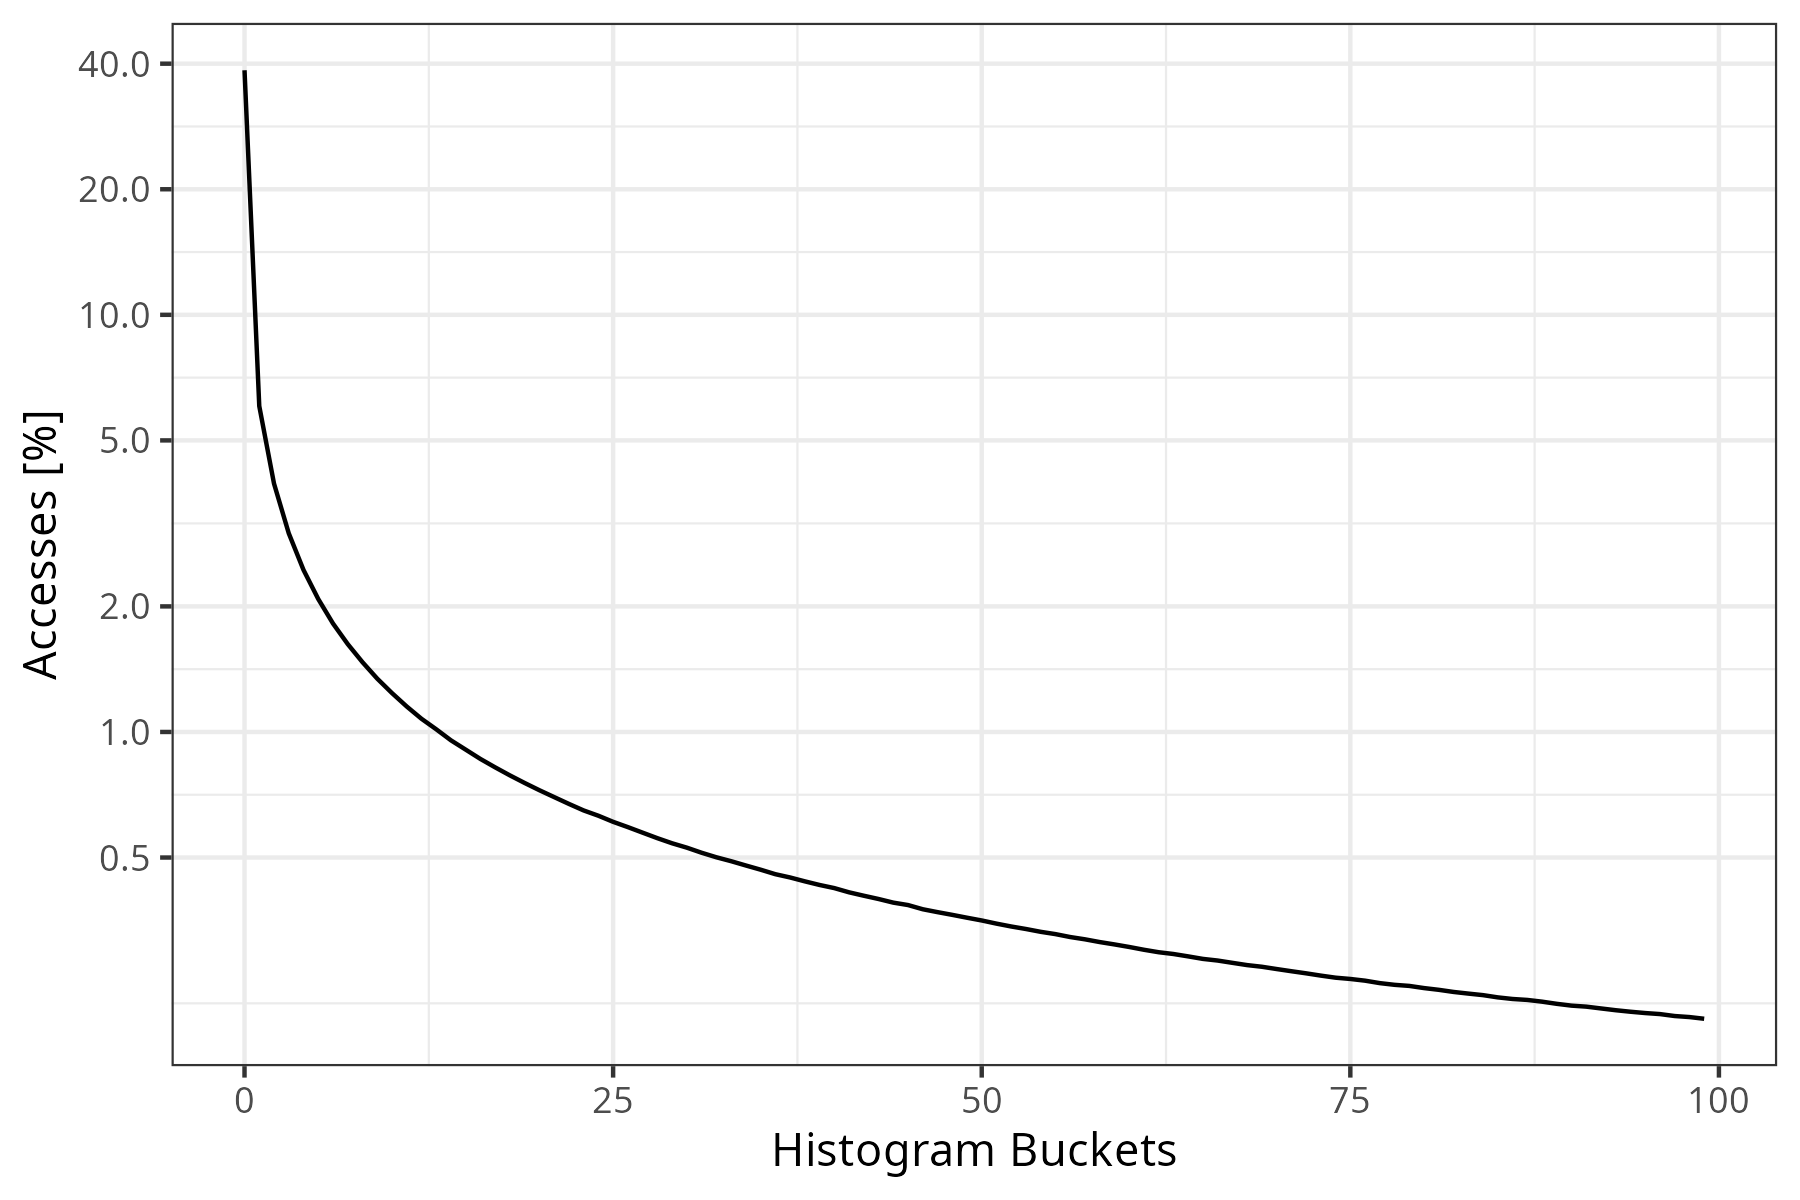
\includegraphics[width=\textwidth]{figures/pmf/rejection.png}
        \caption{Rejection}
    \end{subfigure}

    \label{fig:pmf-graphs}
\end{figure}

\paragraph{Log-scaled graphs}These graphs allows for identifaction of systematic biases in data generation (as explained in Chapter \ref{chapter:background}). The y-axis represents the \textit{counts} and the x-axis the 
\textit{histogram entries} (or "buckets") for all ranks, as shown in figure \ref{fig:log-log}. As was the case before, only FIO and the condensed table lookoup implementations have glaring 
deviations from the expected straight line.

\begin{figure}
    % First row
    \centering
    \begin{subfigure}{0.46\textwidth}
        \centering
        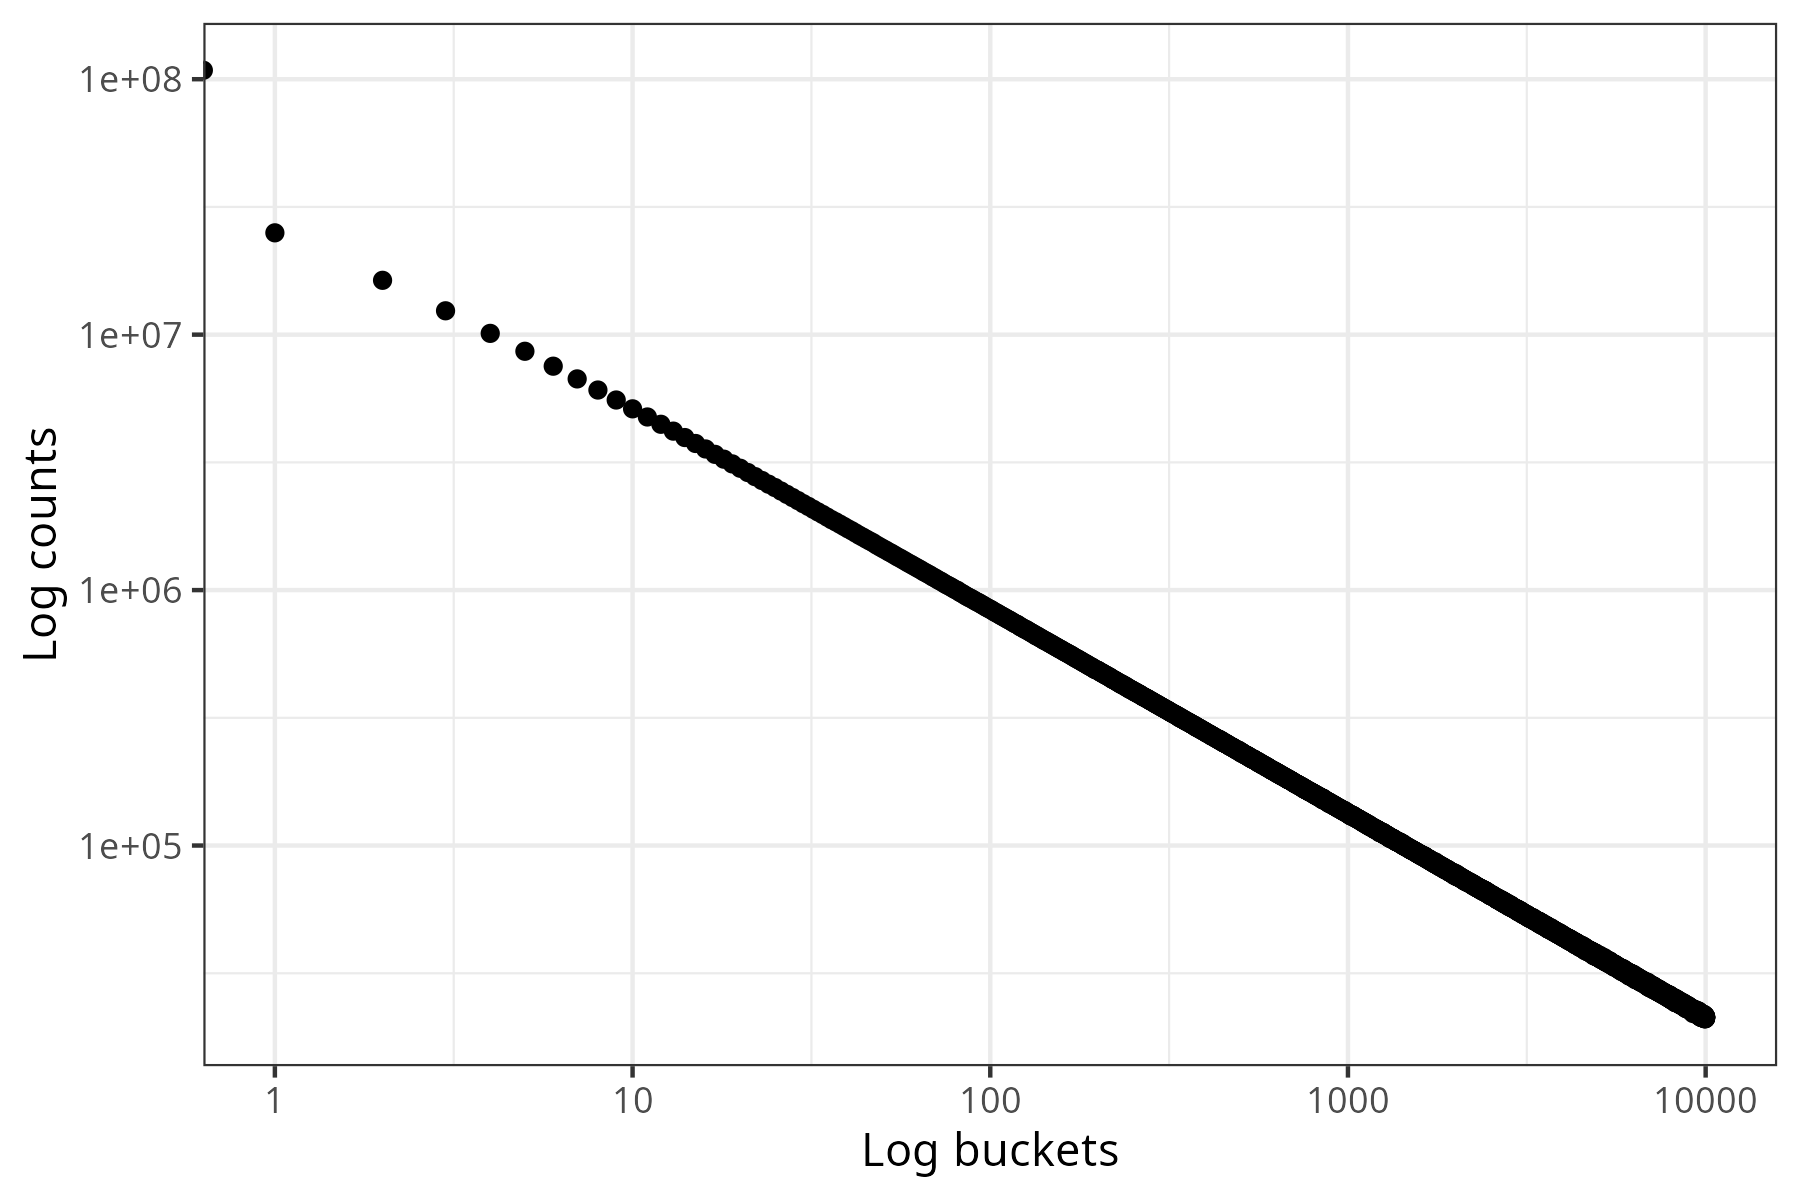
\includegraphics[width=\textwidth]{figures/log-log/apache.png}
        \caption{Rejection-Inversion}
    \end{subfigure}
    \hfill
    \begin{subfigure}{0.46\textwidth}
        \centering
        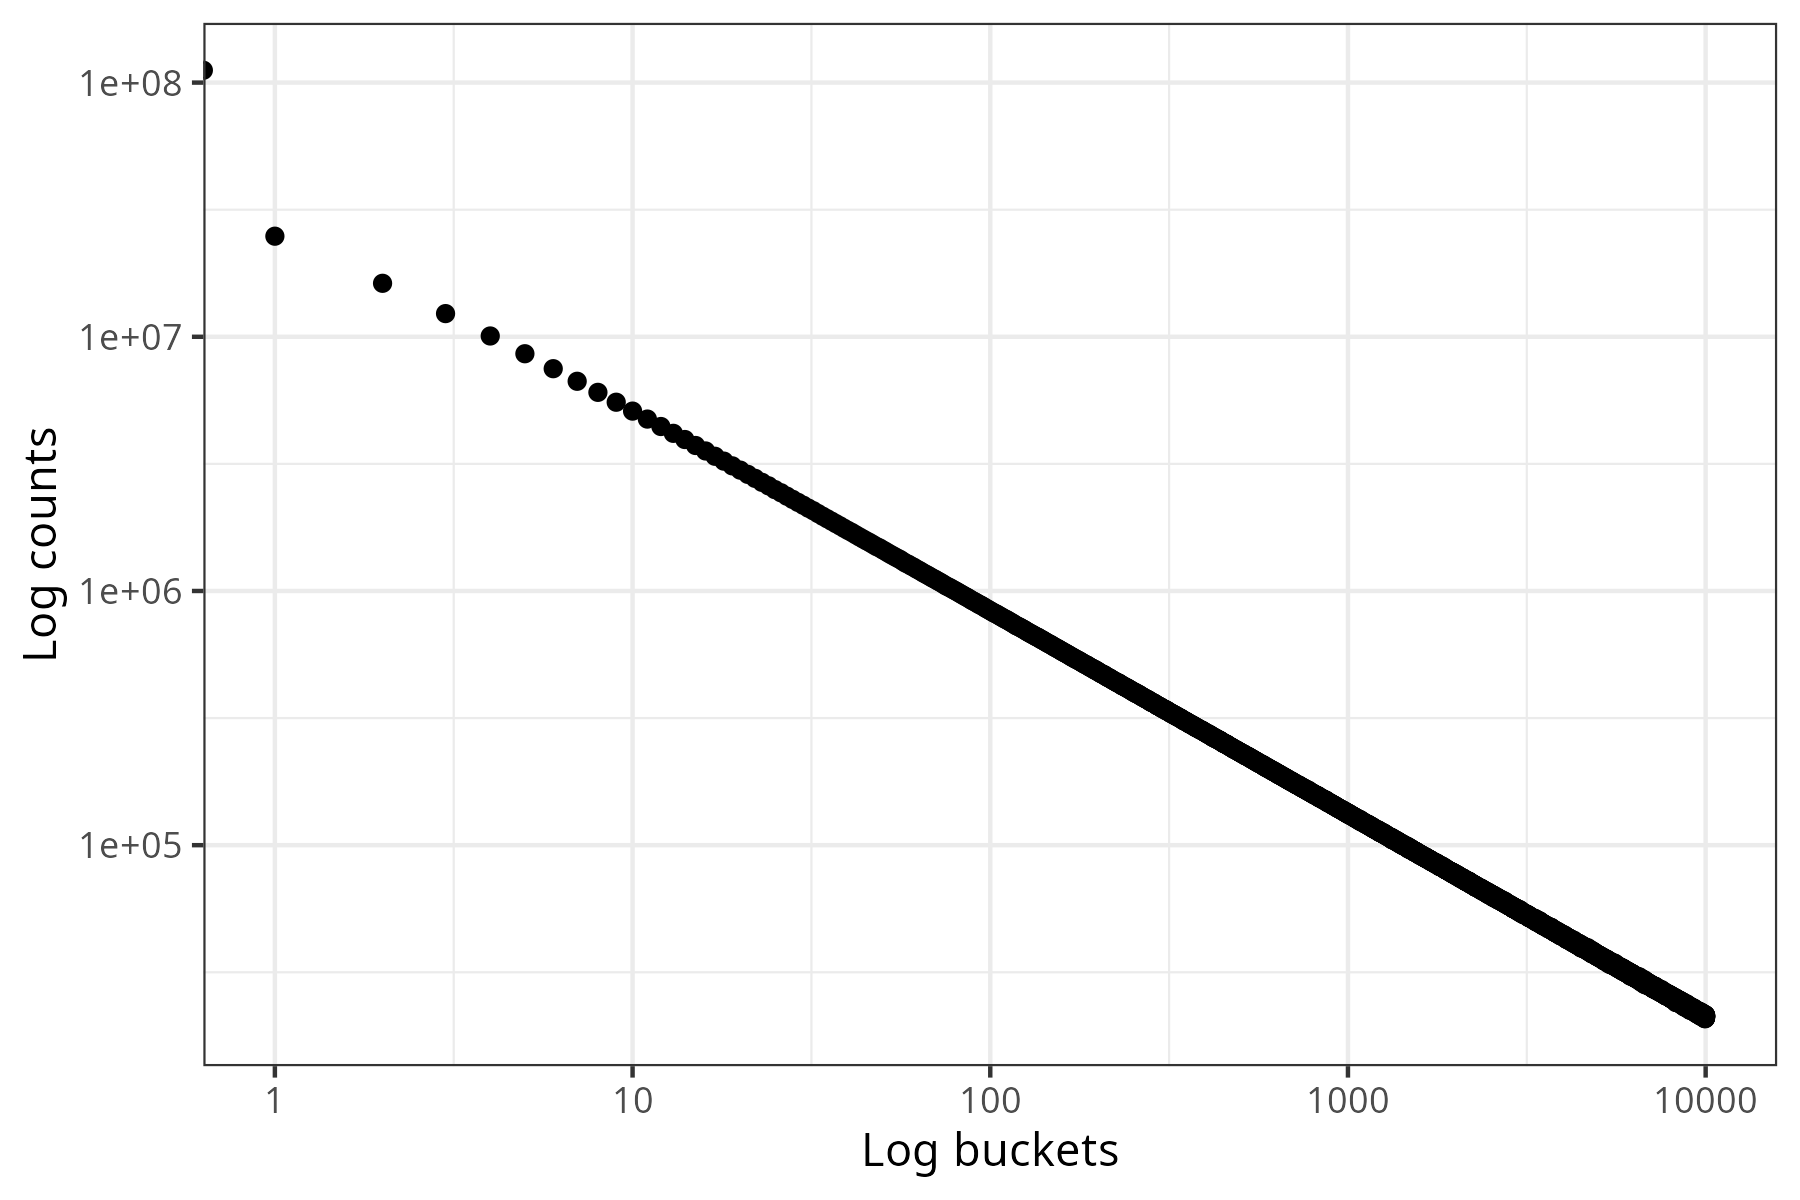
\includegraphics[width=\textwidth]{figures/log-log/ycsb.png}
        \caption{YCSB}
    \end{subfigure}
    
    \vspace{1em}

    % Second row
    \begin{subfigure}{0.46\textwidth}
        \centering
        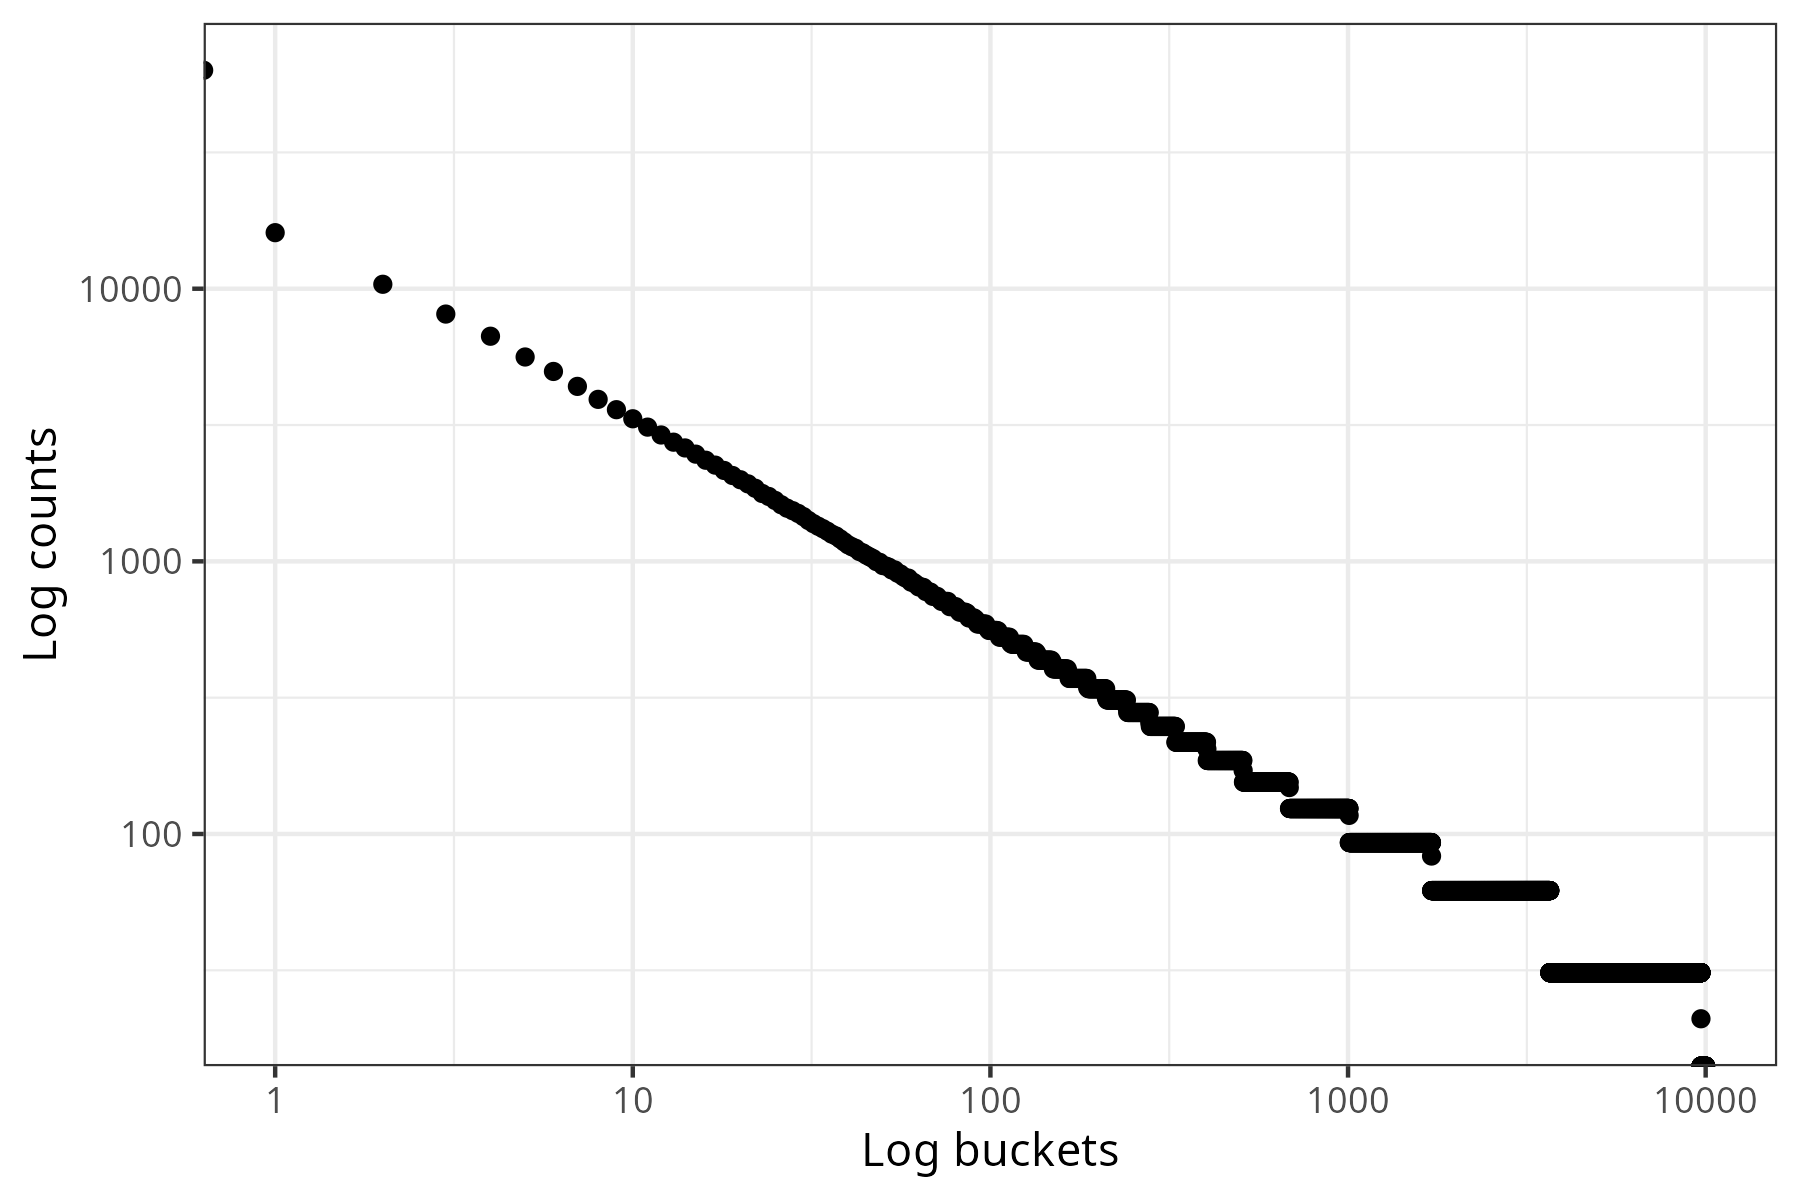
\includegraphics[width=\textwidth]{figures/log-log/fio.png}
        \caption{FIO}
    \end{subfigure}
    \hfill
    \begin{subfigure}{0.46\textwidth}
        \centering
        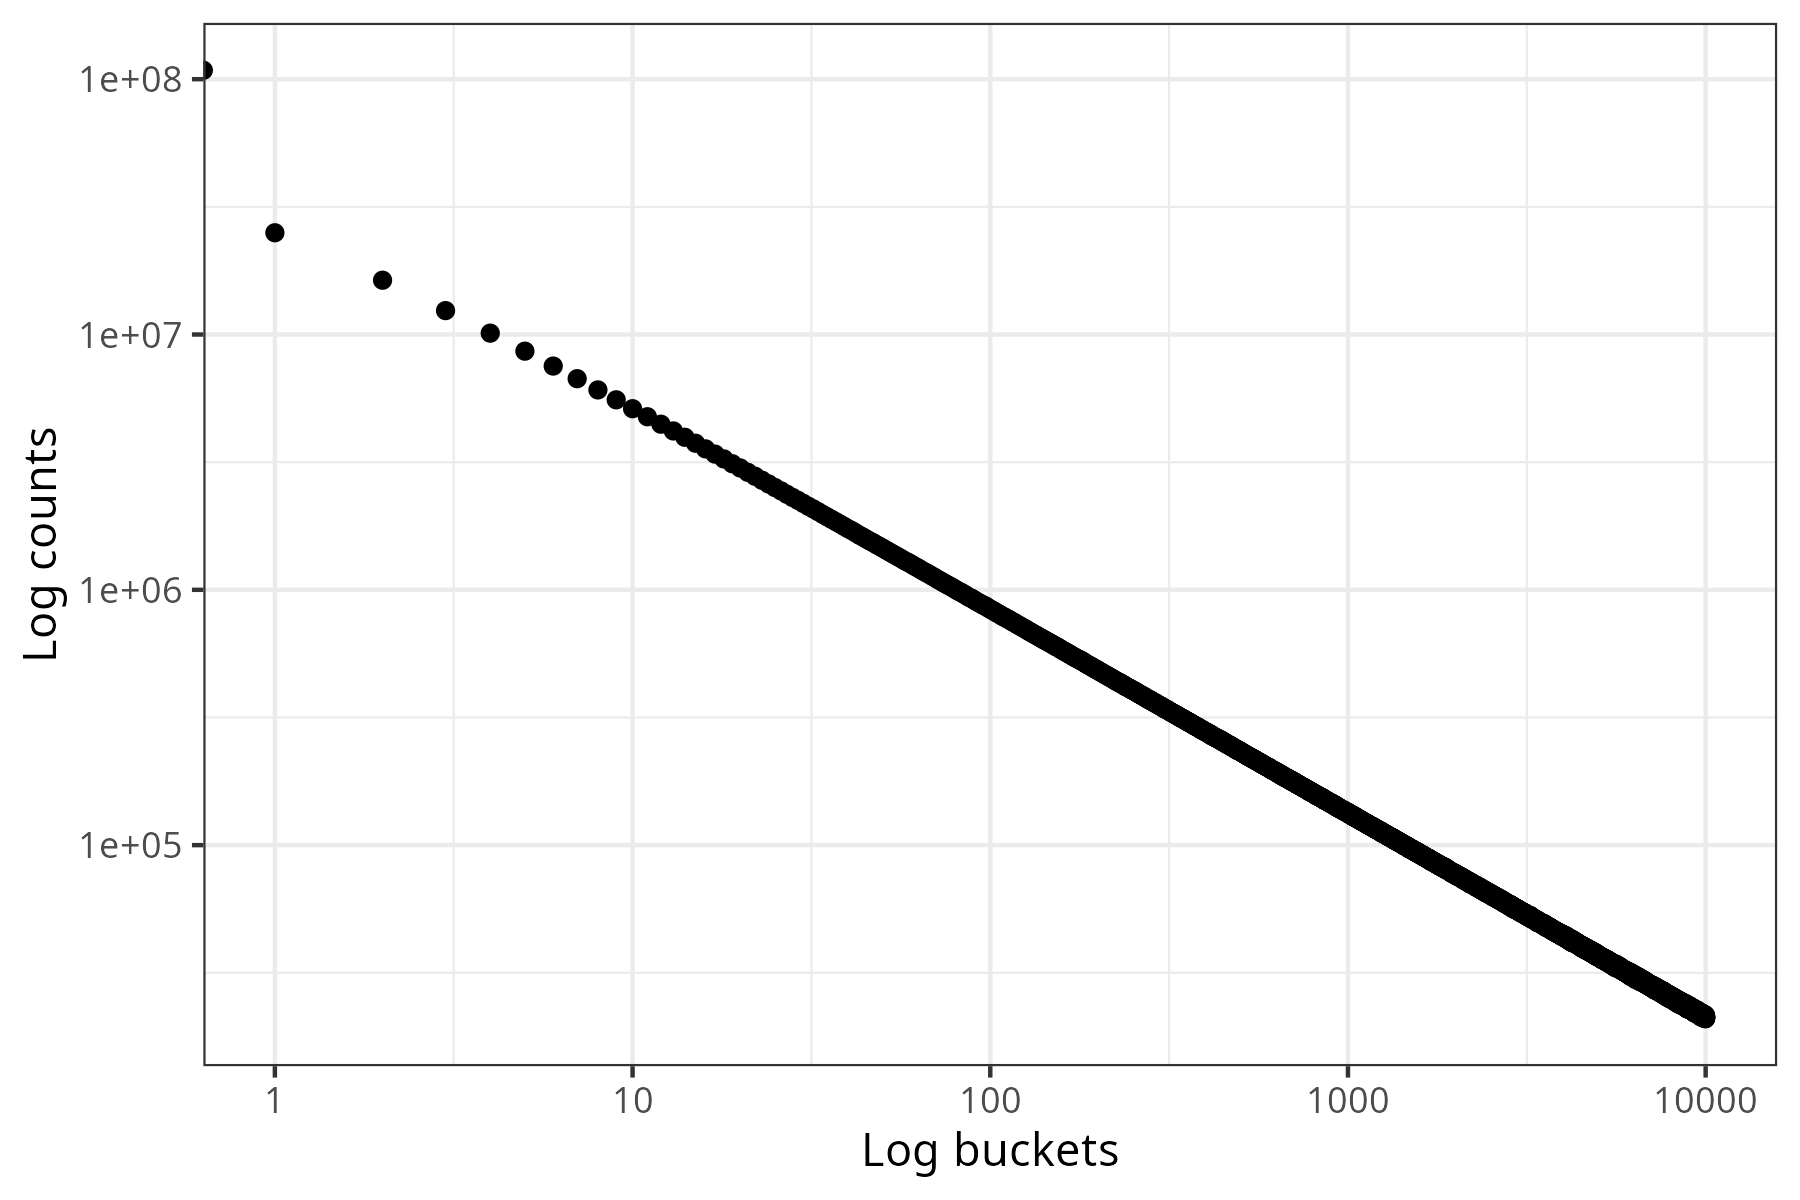
\includegraphics[width=\textwidth]{figures/log-log/sysbench.png}
        \caption{Sysbench}
    \end{subfigure}
    
    \vspace{1em}

    % Third row
    \begin{subfigure}{0.46\textwidth}
        \centering
        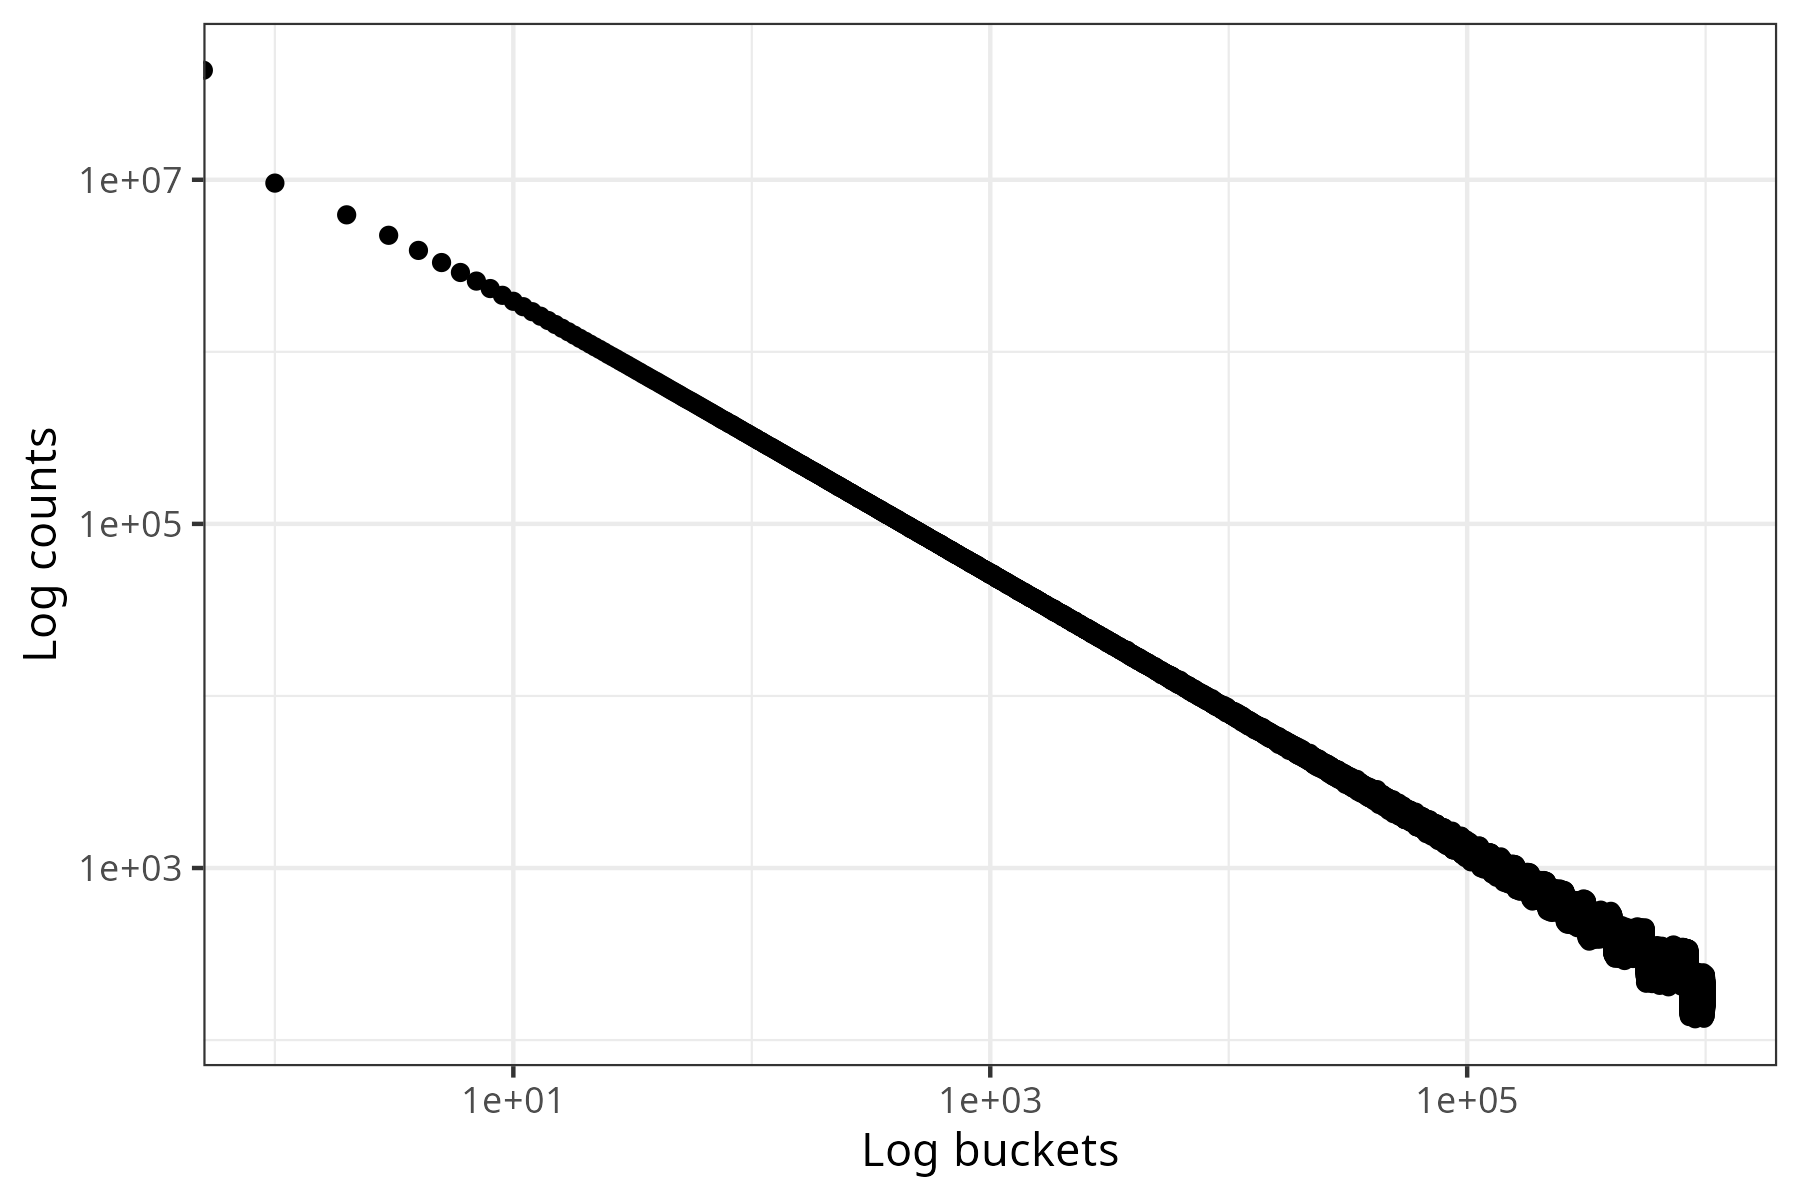
\includegraphics[width=\textwidth]{figures/log-log/marsaglia.png}
        \caption{Condensed Table Lookup}
    \end{subfigure}
    \hfill
    \begin{subfigure}{0.46\textwidth}
        \centering
        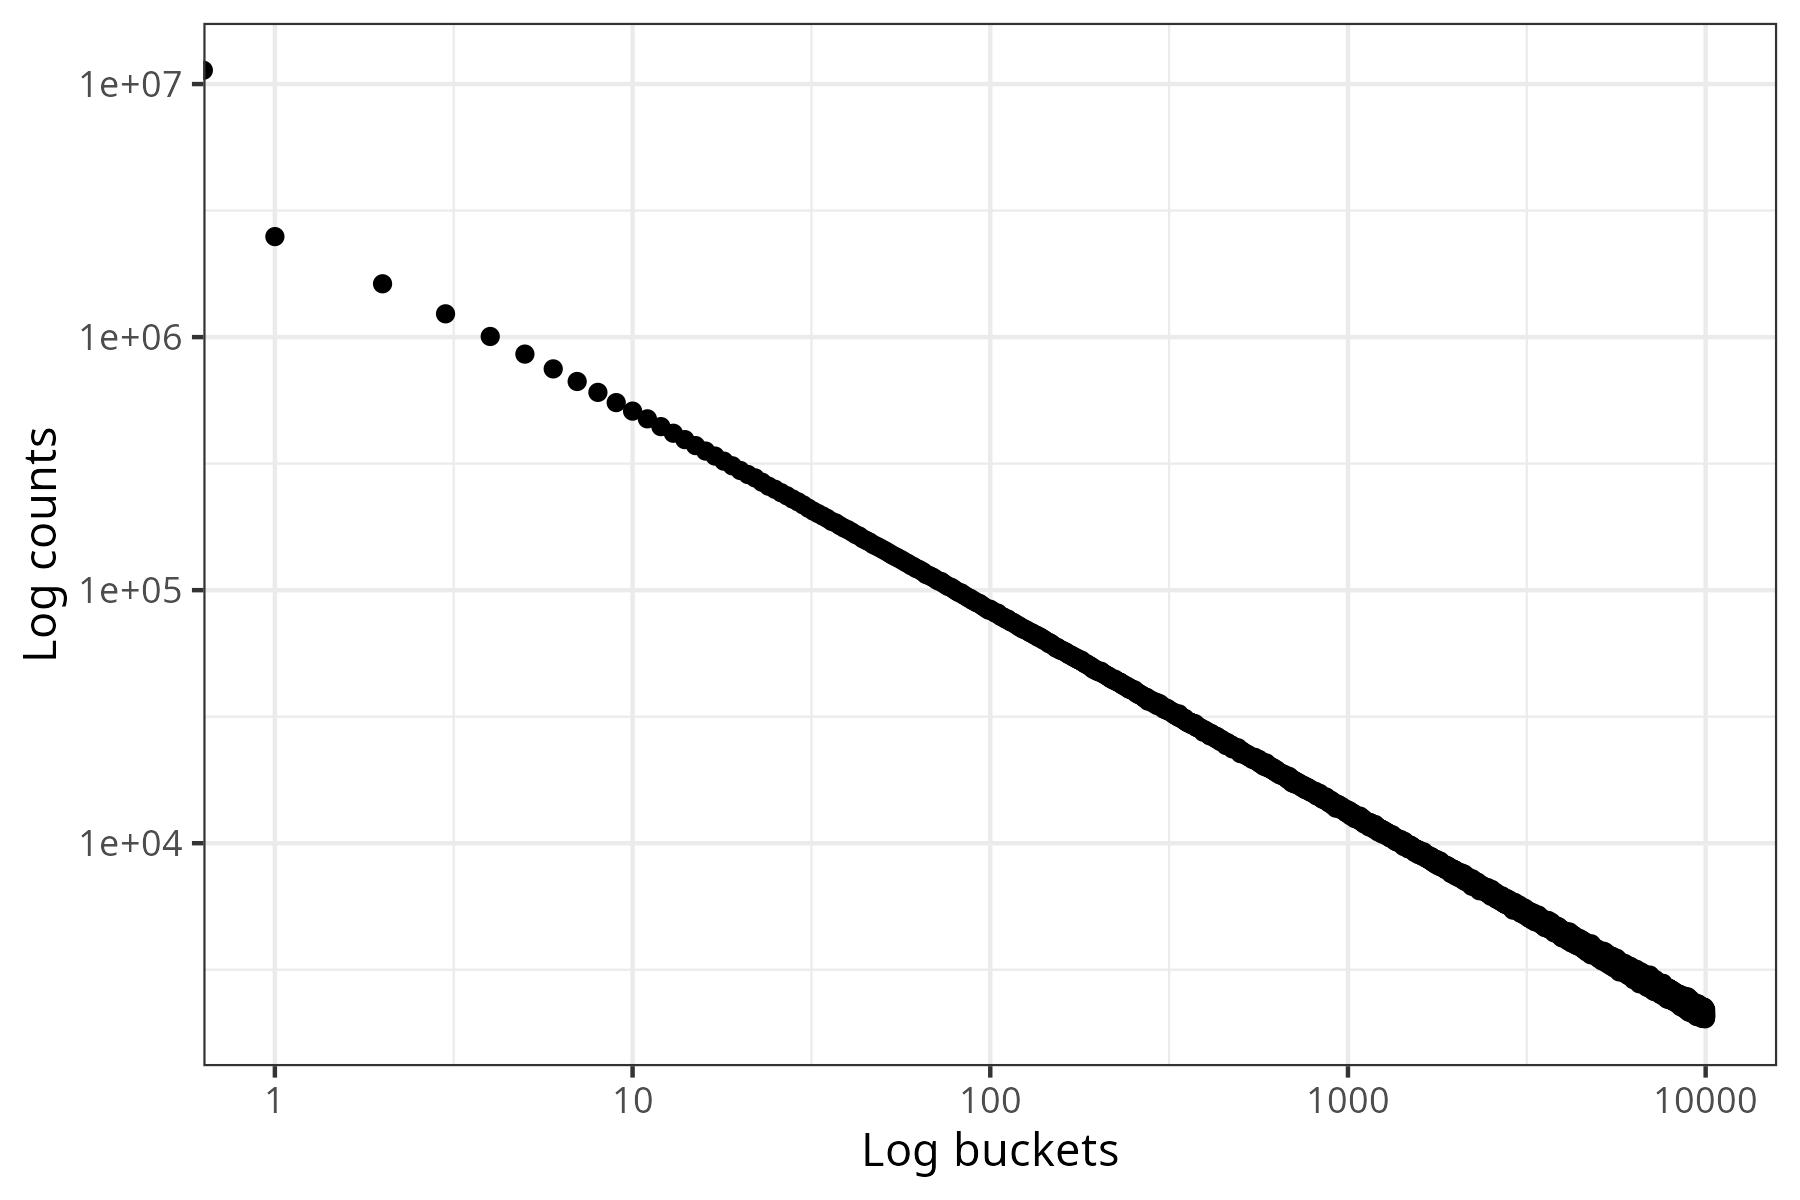
\includegraphics[width=\textwidth]{figures/log-log/rejection.png}
        \caption{Rejection Sampling}
    \end{subfigure}
    
    
    \caption{Log-log plots of the performance of the 6 different variate generators.}
    \label{fig:log-log}
\end{figure}

\paragraph{Frequency Ratio Analysis} 
To further analyse how the accuracy varies within the domain of the distribution, a frequency ratio analysis is conducted. This is done by plotting the ratio of the empirical frequency to the 
theoretical frequency (see Equation \ref{eqt:zm_prob}) against the rank of the variate - $\frac{f_{emp}(k)}{f_{theo}(k)}$, where $k$ denotes the rank.

The graphs in figure \ref{fig:ratio-graphs} show the results for the 6 variate generators.
Clearly, the more problematic distribution is once again FIO, while other implementations fluctuate around 1.0 - the expected value. Observing the equation \ref{eqt:zm_prob} and the graph
of \textit{FIO} in figure \ref{fig:pmf_graphs} dismystifies the problem: The probability stays constants for long stretches of the domain, whereas the real distribution ever so decreases. This
in turn makes the ratio of the empirical to the theoretical frequency increase, before falling off again. 

\begin{figure}[t]
    % First row
    \centering
    \begin{subfigure}{0.46\textwidth}
        \centering
        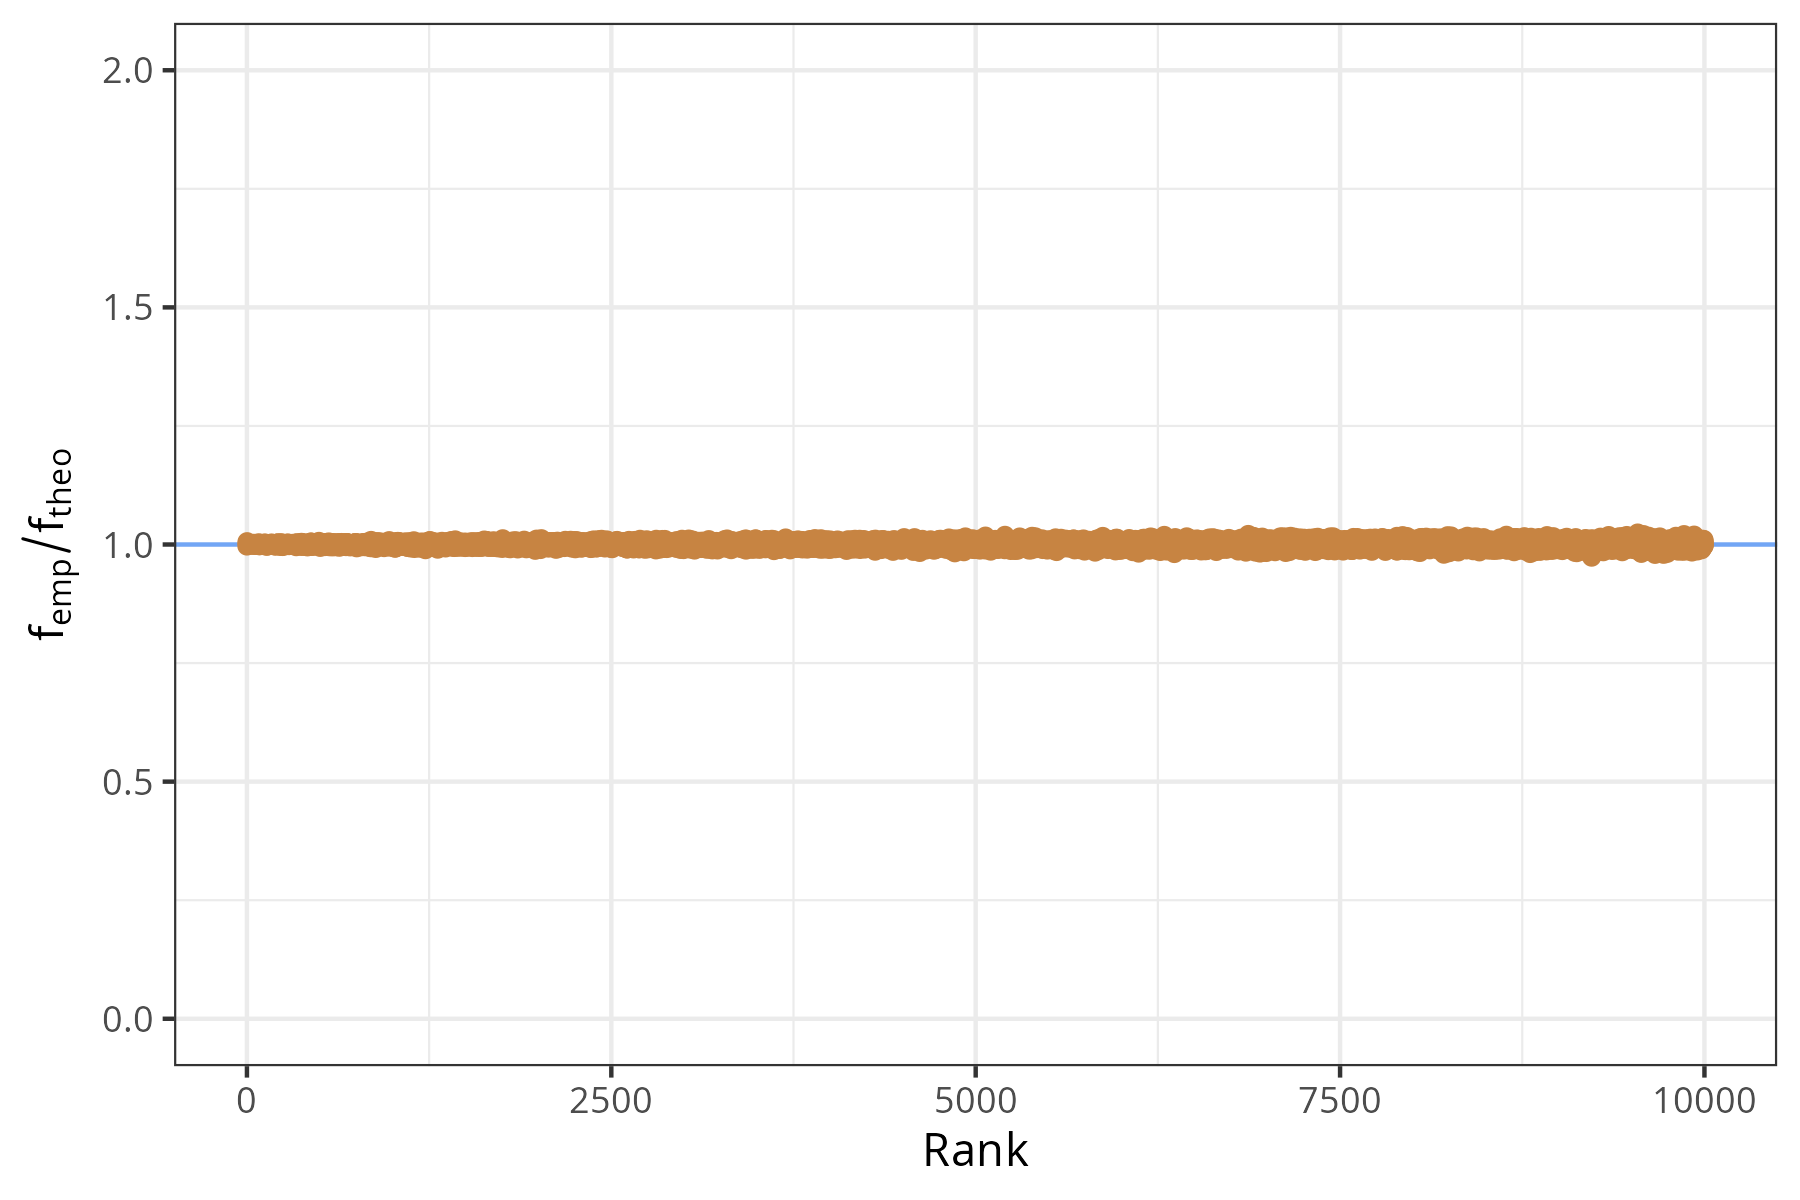
\includegraphics[width=\textwidth]{figures/ratio/apache.png}
        \caption{Rejection inversion}
    \end{subfigure}
    \hfill
    \begin{subfigure}{0.46\textwidth}
        \centering
        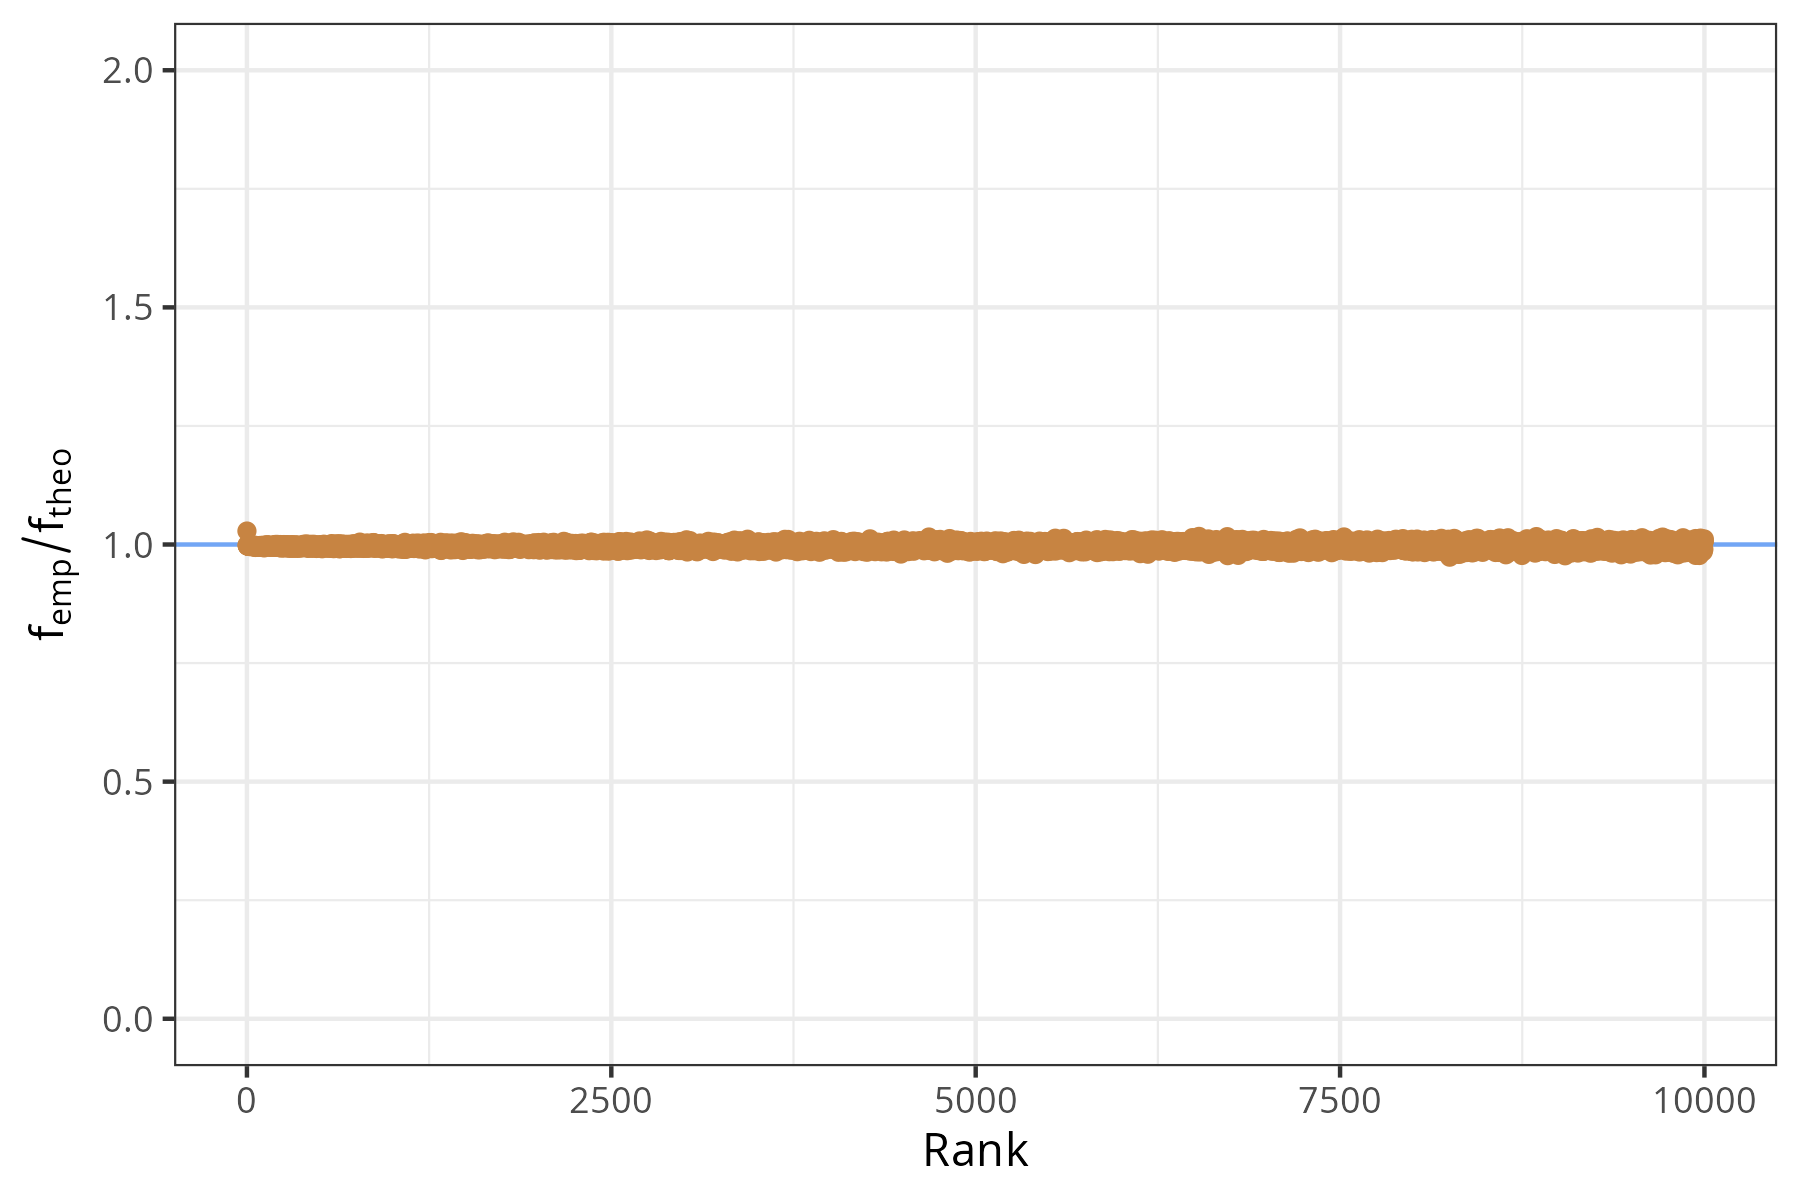
\includegraphics[width=\textwidth]{figures/ratio/ycsb.png}
        \caption{YCSB}
    \end{subfigure}
    
    \vspace{1em} % Space between rows
    
    % Second row
    \begin{subfigure}{0.46\textwidth}
        \centering
        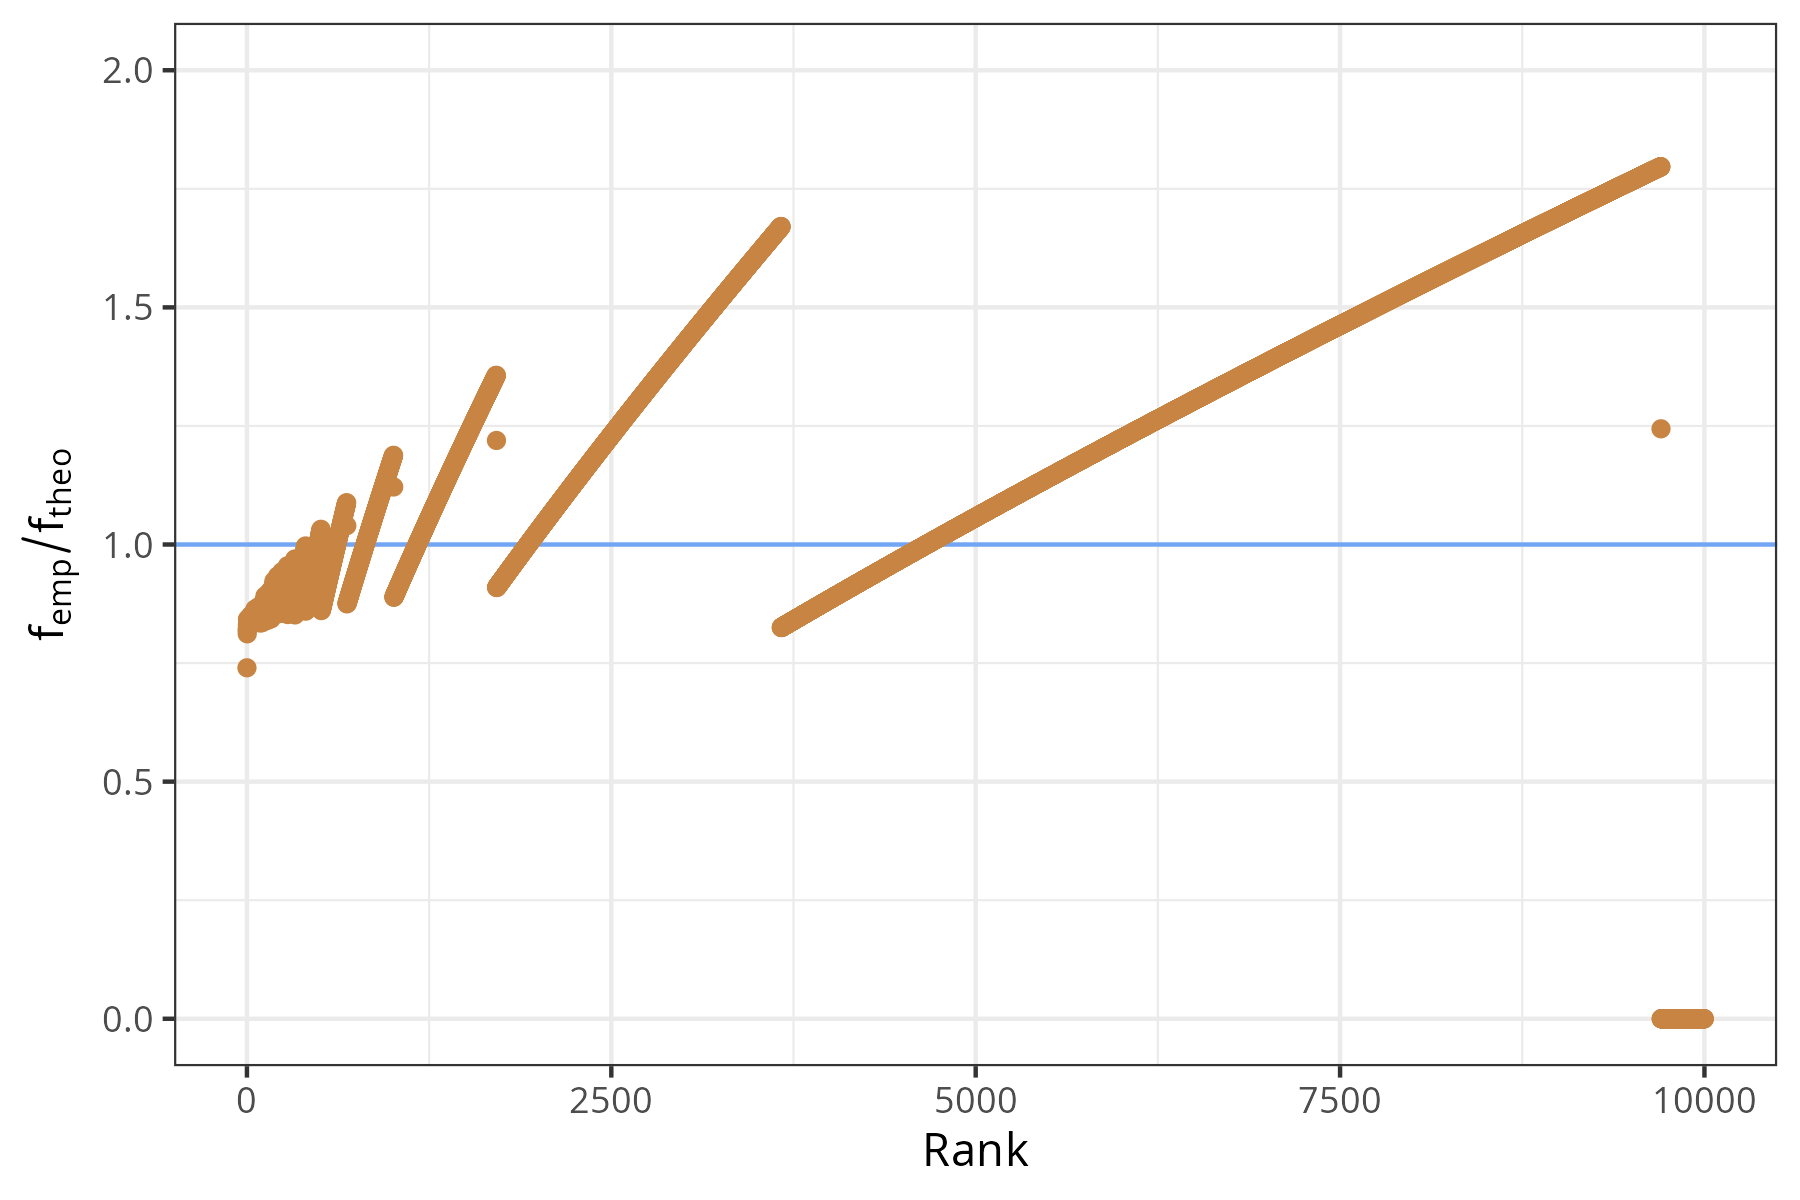
\includegraphics[width=\textwidth]{figures/ratio/fio.png}
        \caption{FIO}
    \end{subfigure}
    \hfill
    \begin{subfigure}{0.46\textwidth}
        \centering
        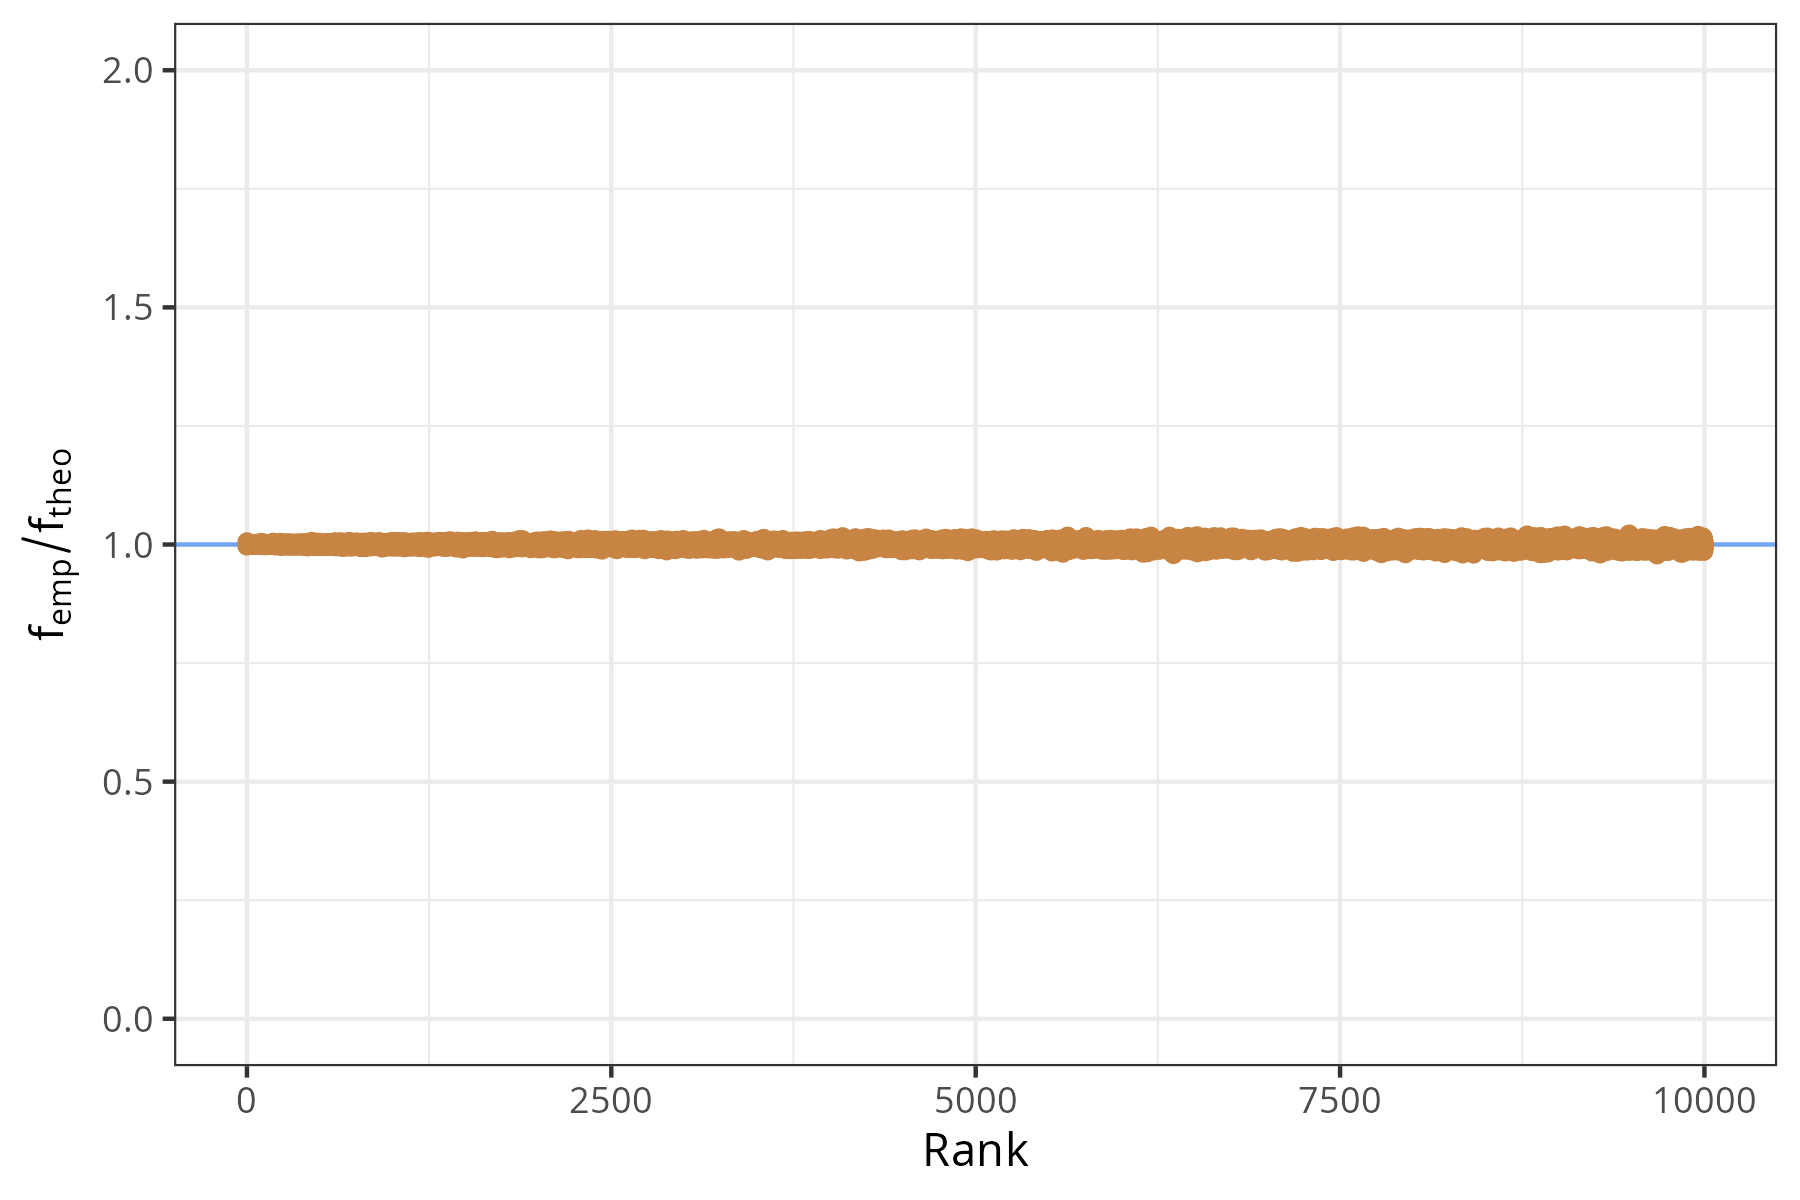
\includegraphics[width=\textwidth]{figures/ratio/sysbench.png}
        \caption{Sysbench}
    \end{subfigure}

    \vspace{1em} % Space between rows
    
    % Third row
    \begin{subfigure}{0.46\textwidth}
        \centering
        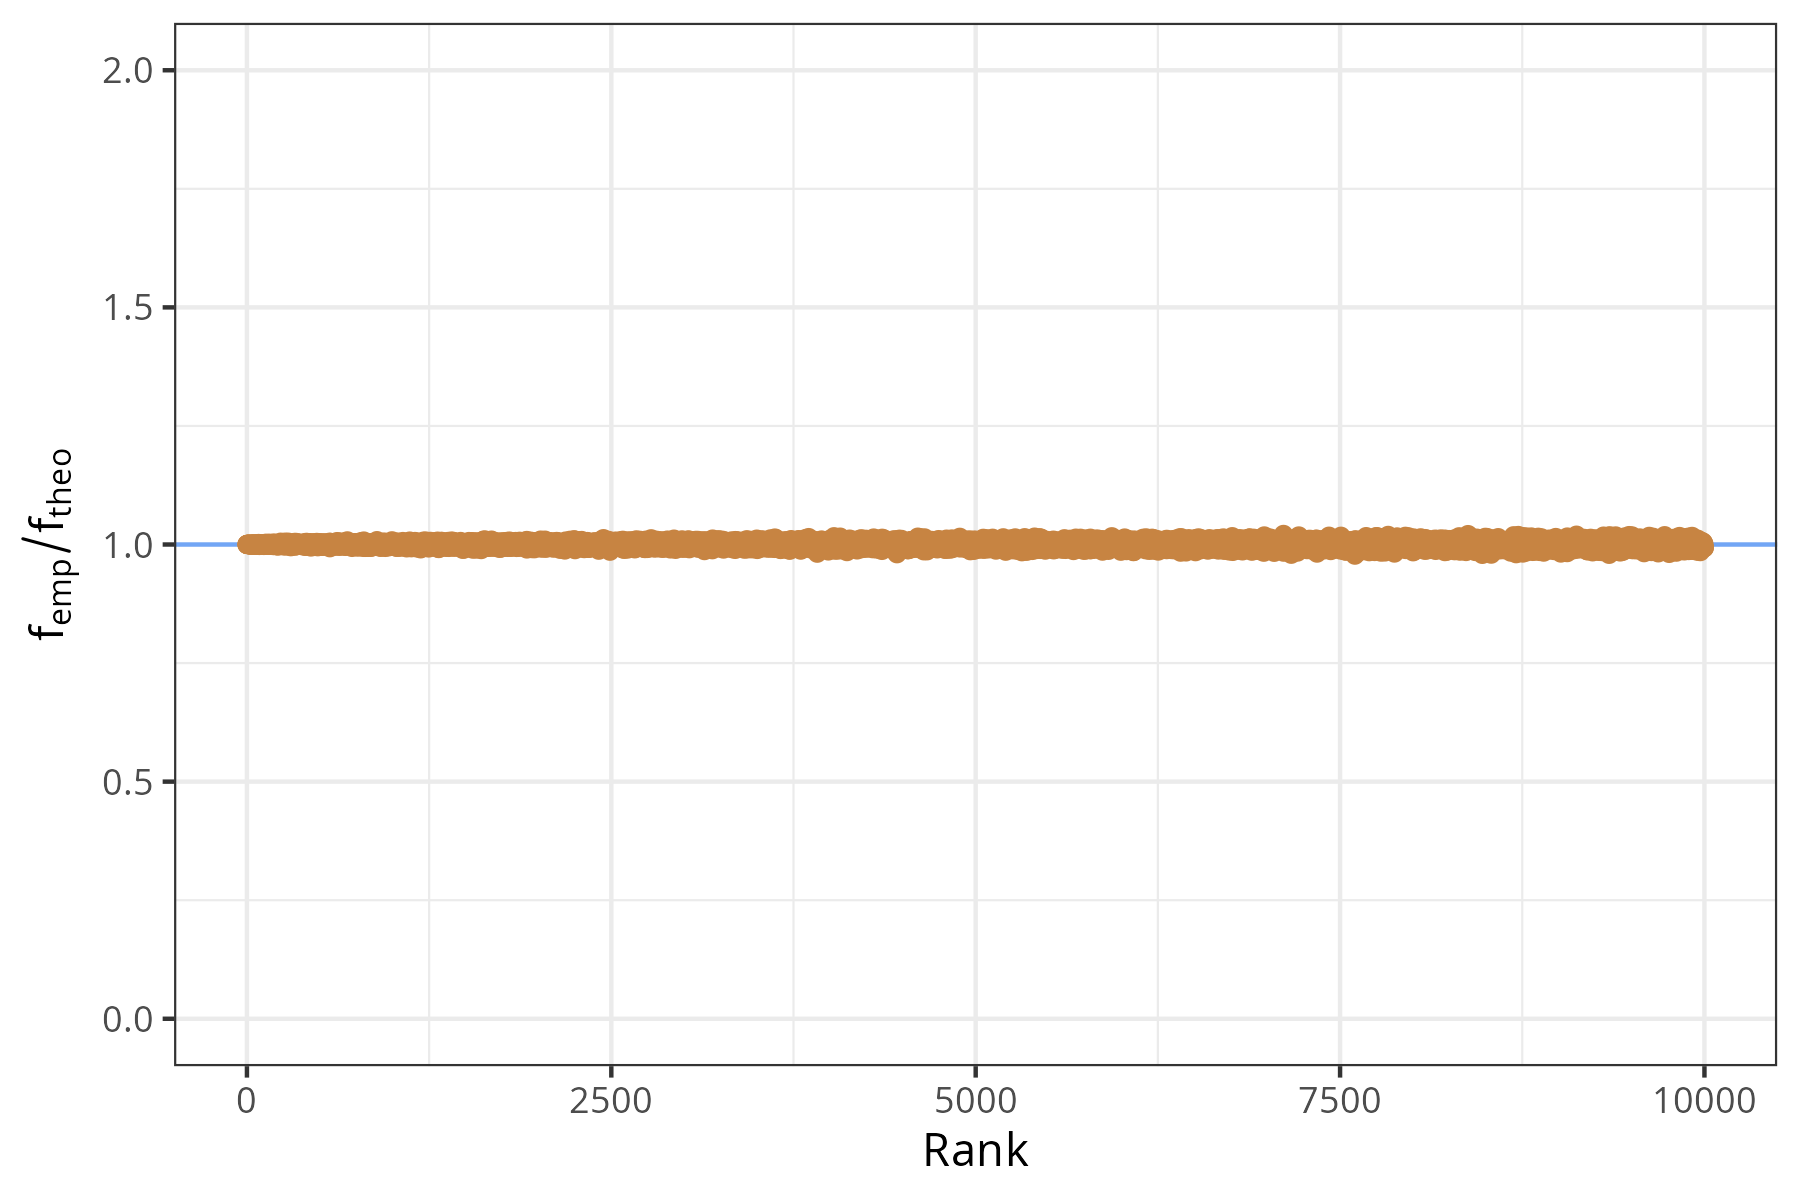
\includegraphics[width=\textwidth]{figures/ratio/marsaglia.png}
        \caption{Condensed Table Lookup}
    \end{subfigure}
    \hfill
    \begin{subfigure}{0.46\textwidth}
        \centering
        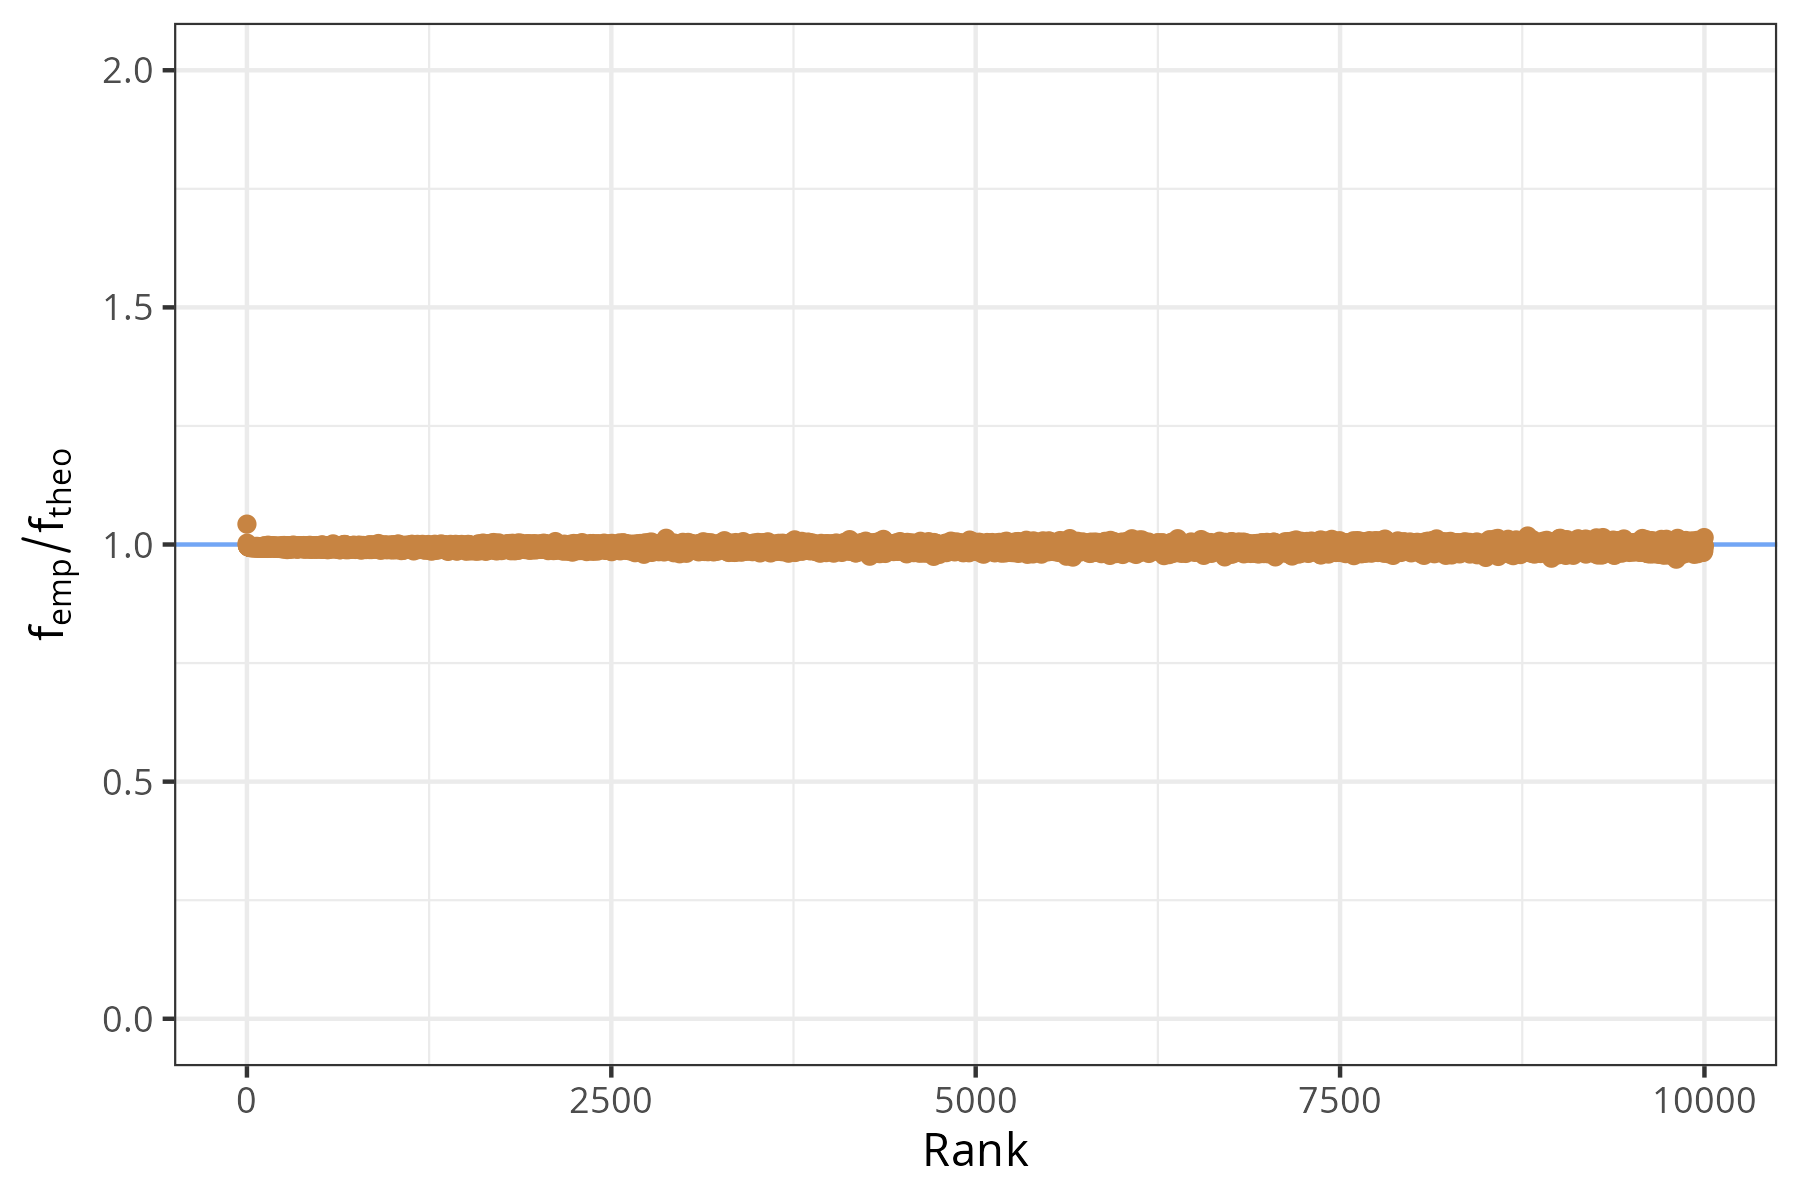
\includegraphics[width=\textwidth]{figures/ratio/rejection.png}
        \caption{Rejection}
    \end{subfigure}

    \caption{All distributions have support size $10^6$ and have $10^9$ samples}
    \label{fig:ratio-graphs}
\end{figure}

\paragraph{Quantitative Criteria} 
First follows the \textbf{Kolmogorov-Smirnov test} in Figure \ref{fig:ks_graphs} and the \textbf{total variation distance} in Figure \ref{fig:tvd-graphs}. From both graphs,
we notice that the FIO implementation is the one that deviates the most from the expected values, while the other implementations are very close to the expected values. Since all but FIO
converge to smaller error values, we can discard the hypothesis that some there are systematic errors and that all implementations are accurate. While there 
is some evidence that moments (such as mean, variance) of self-similar distributions, such as the Zipfian distribution, only very slowly converge to their theoretical values in a sampling environment \cite{crovellaSimulationsHeavyTailedWorkloads2000}
, it seems that for the \textit{Rejection Inversion} (Sysbench, AuctionMark), \textit{Rejection} and \textit{approximative} (YCSB, FIO) sampling algorithms, the distributions are very close to the expected values given enough samples. 
The table \ref{tab:accuracy-results} summarizes the results for sample size = $10^9$.

\begin{figure}[t]
    % First row
    \centering
    \begin{subfigure}{0.46\textwidth}
        \centering
        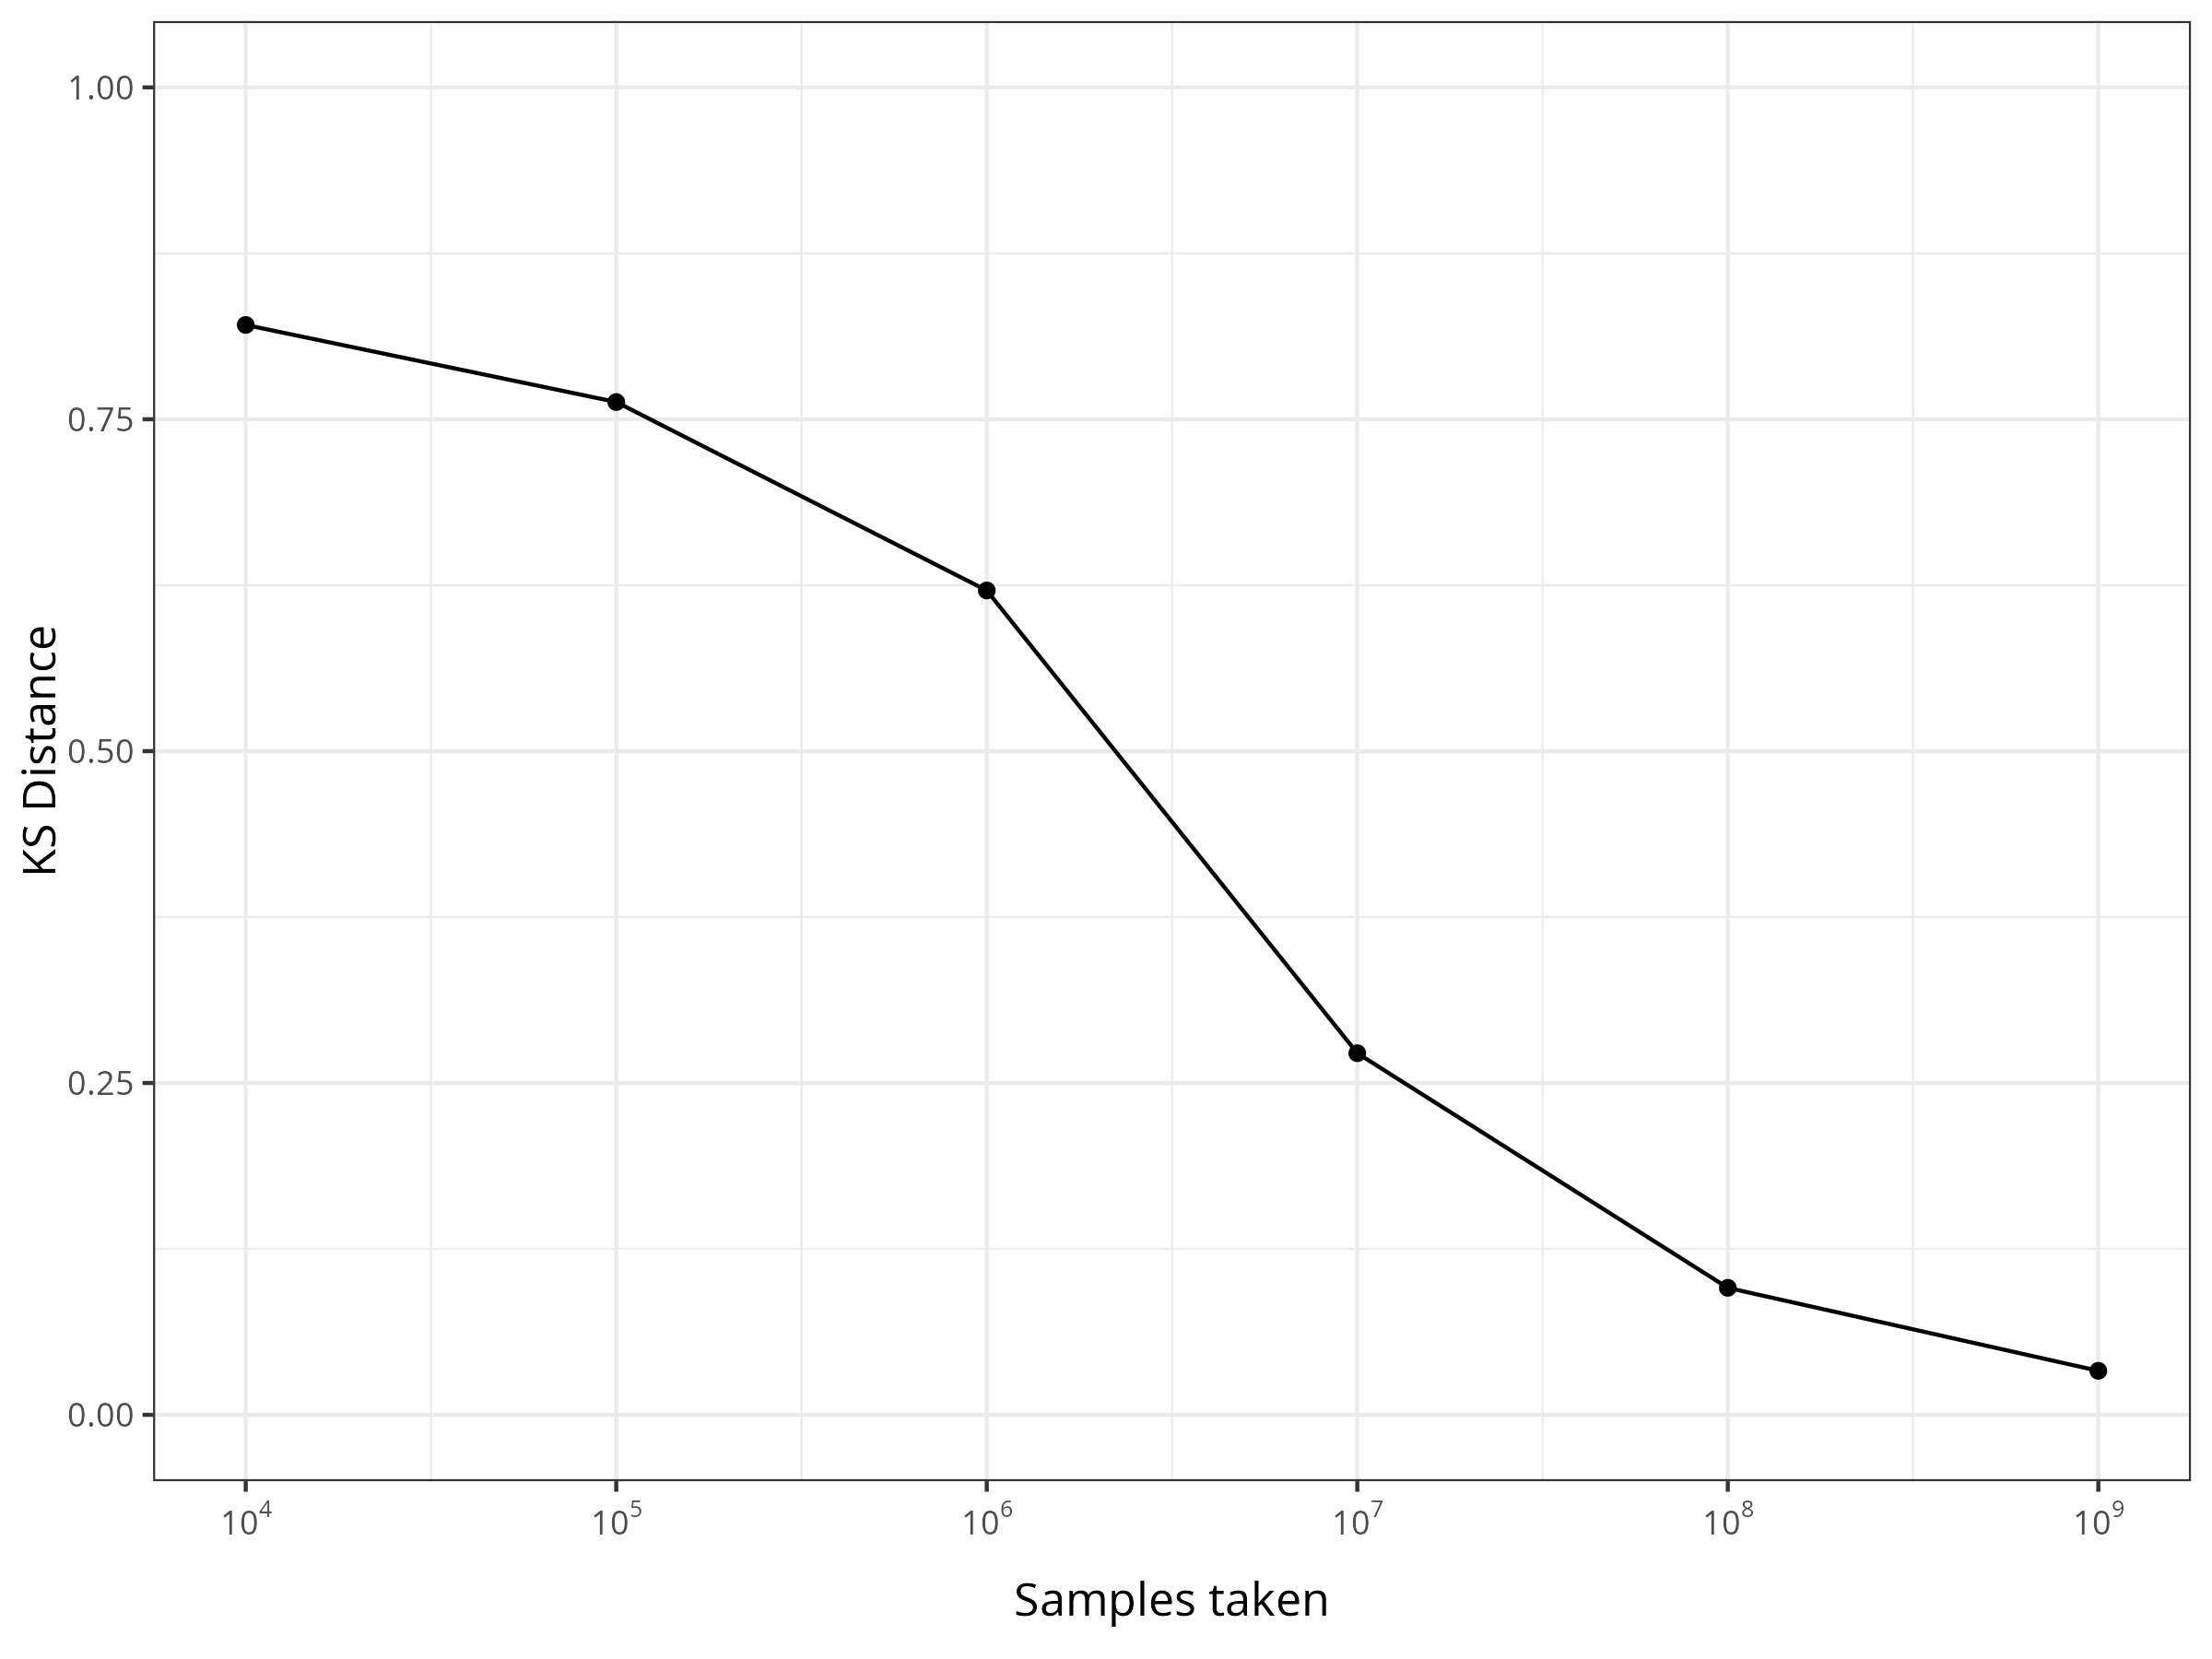
\includegraphics[width=\textwidth]{figures/ks/apache.png}
        \caption{Rejection-Inversion}
    \end{subfigure}
    \hfill
    \begin{subfigure}{0.46\textwidth}
        \centering
        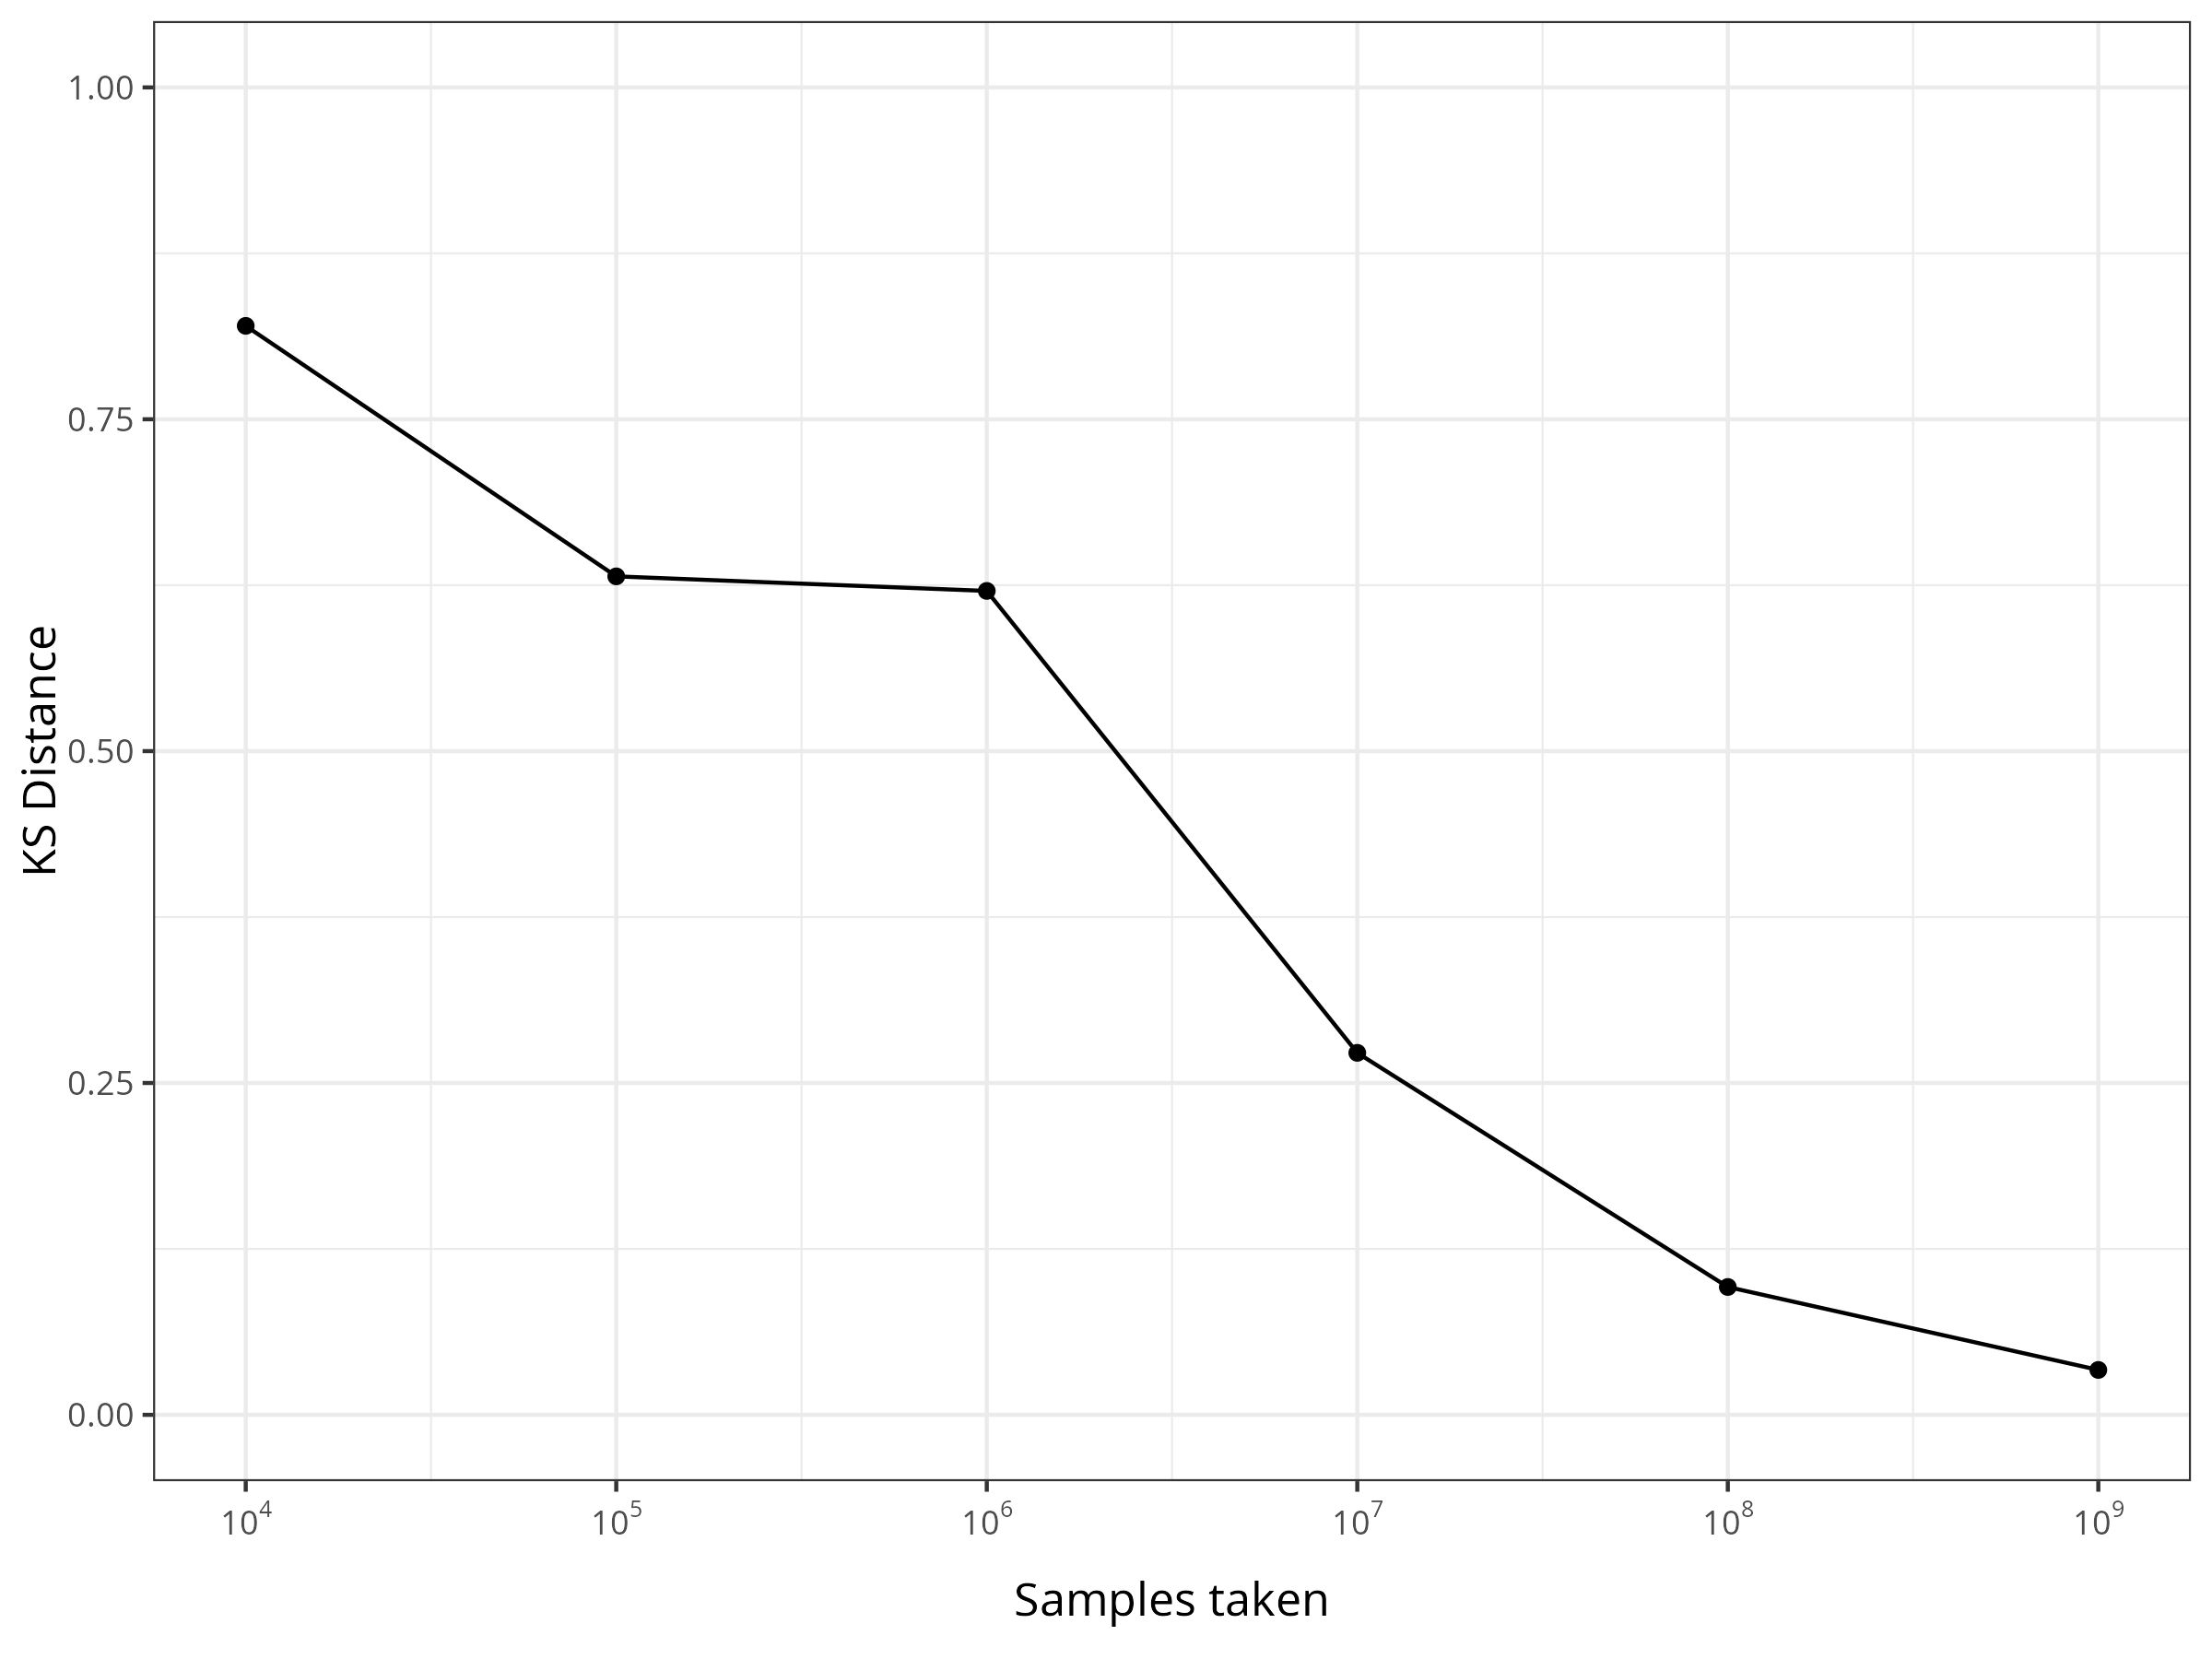
\includegraphics[width=\textwidth]{figures/ks/ycsb.png}
        \caption{YCSB}
    \end{subfigure}
    
    \vspace{1em}

    % Second row
    \begin{subfigure}{0.46\textwidth}
        \centering
        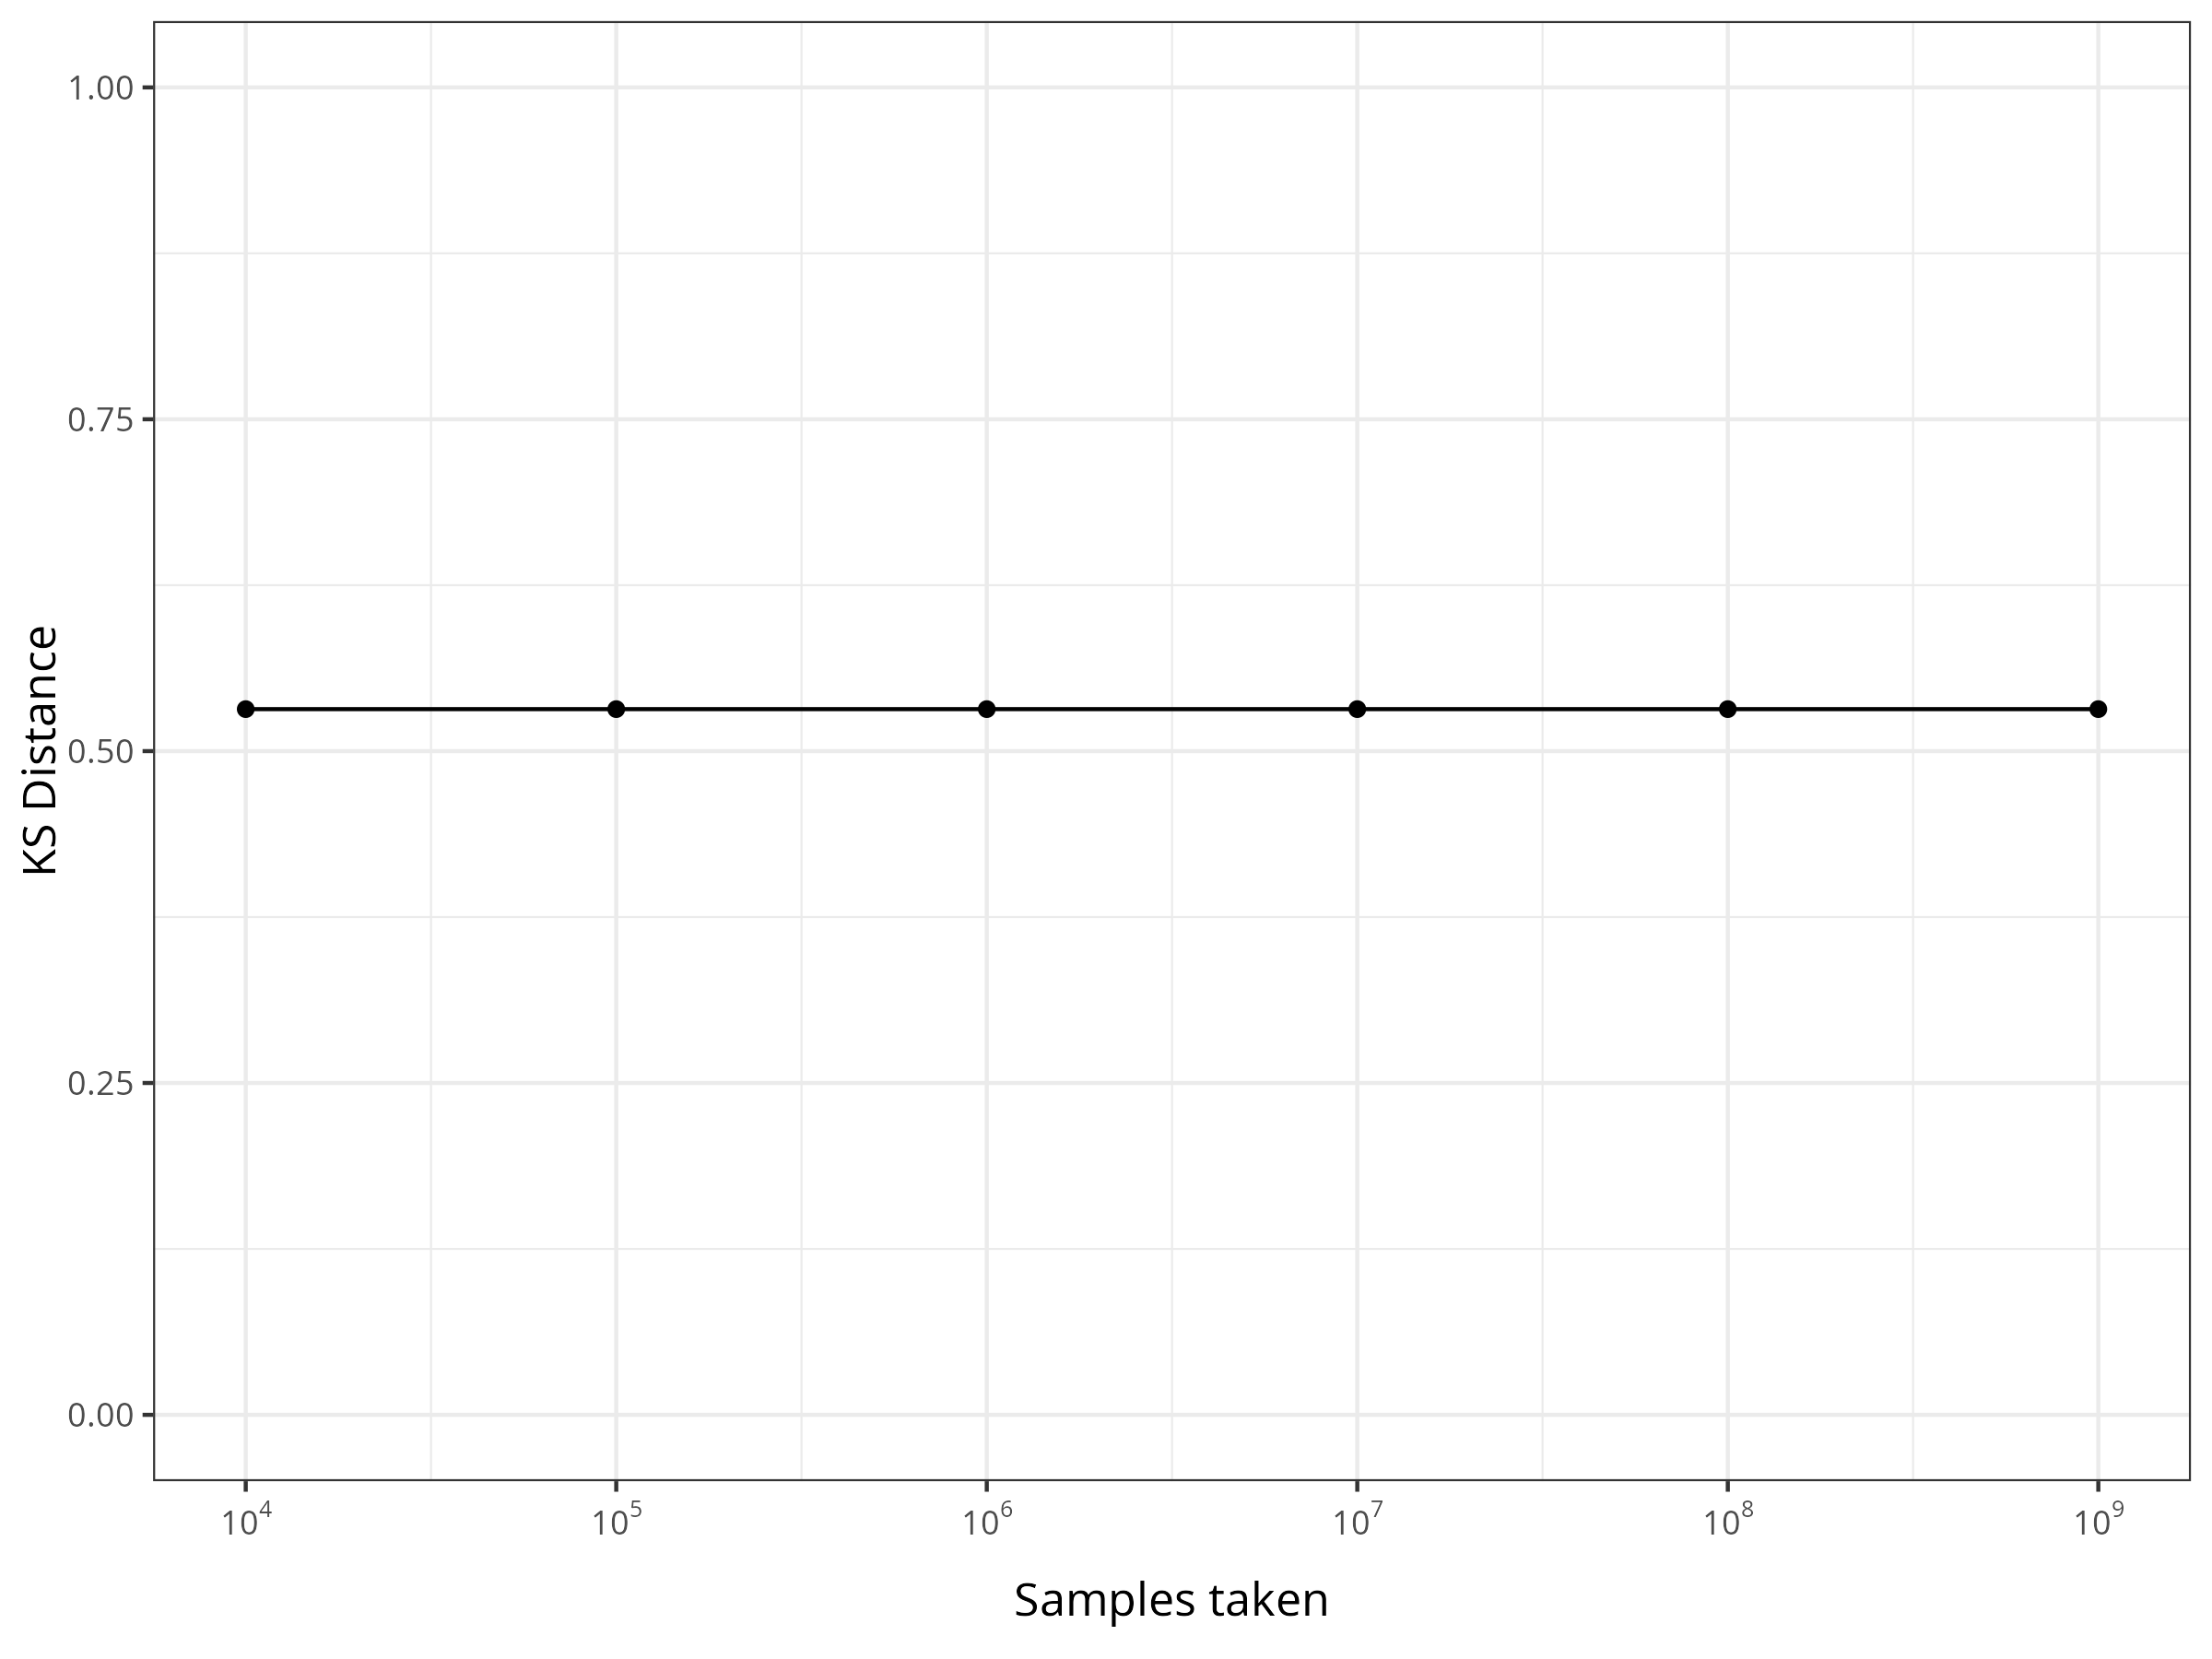
\includegraphics[width=\textwidth]{figures/ks/fio.png}
        \caption{FIO}
    \end{subfigure}
    \hfill
    \begin{subfigure}{0.46\textwidth}
        \centering
        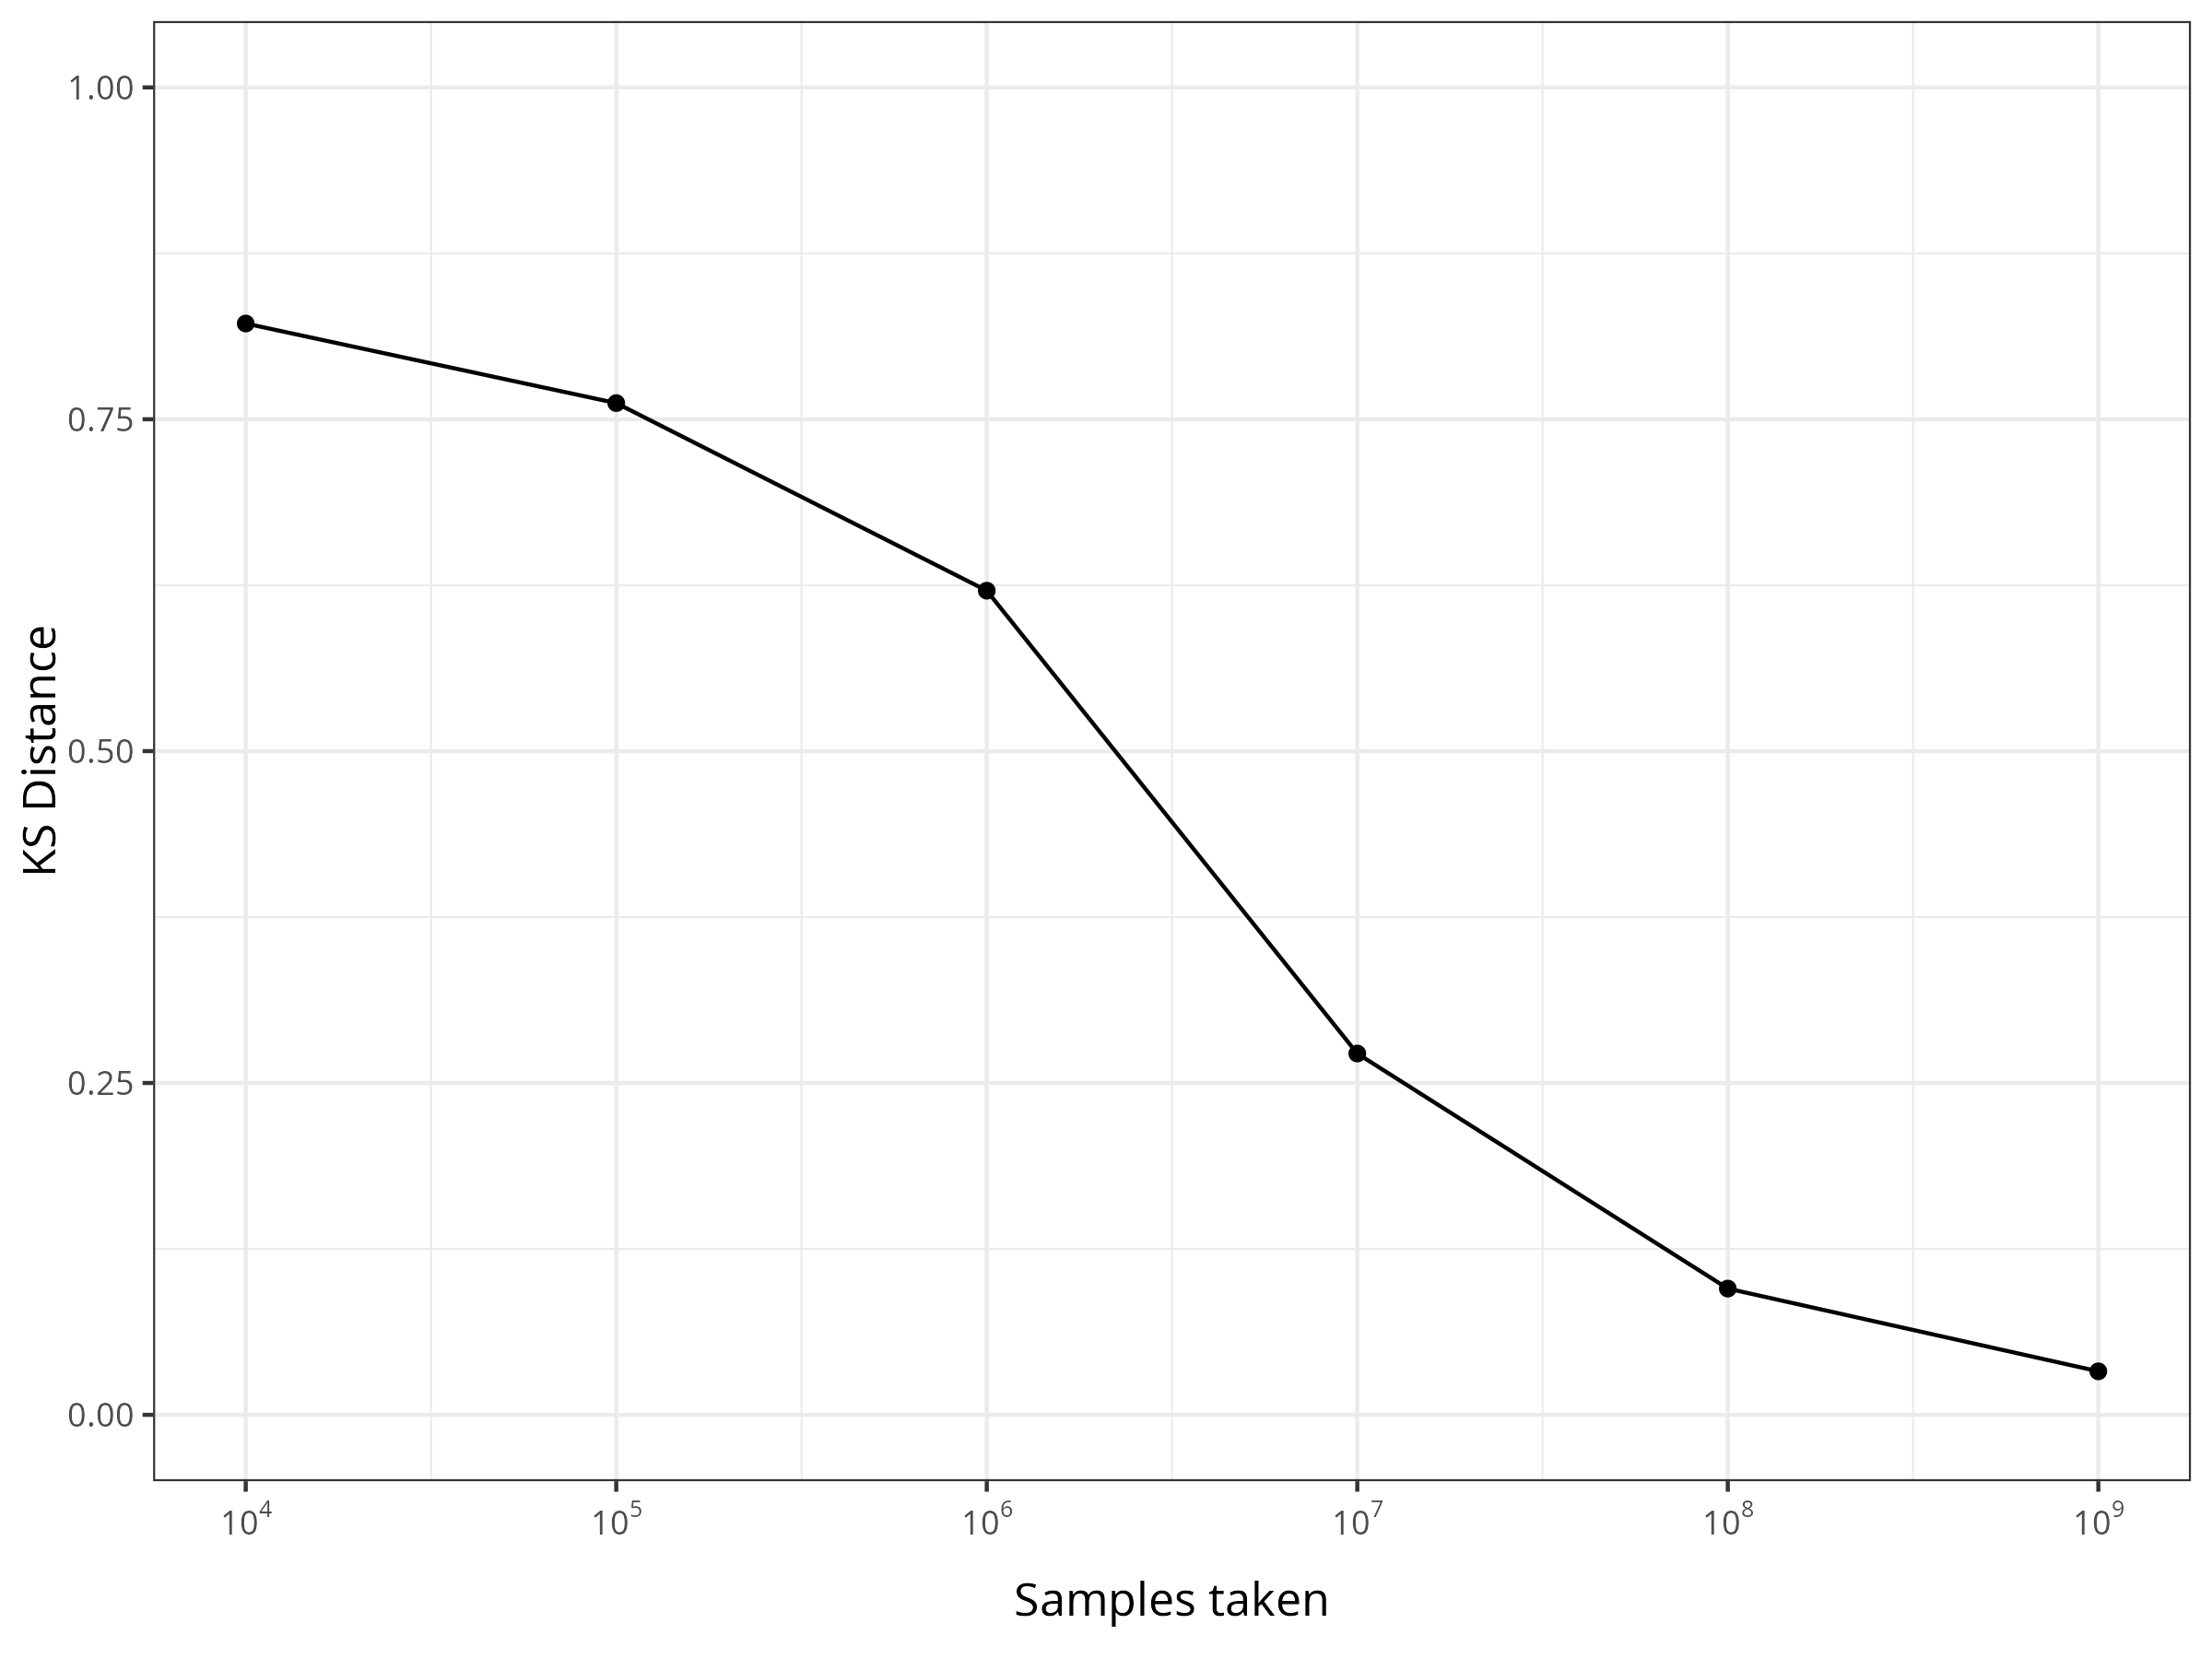
\includegraphics[width=\textwidth]{figures/ks/sysbench.png}
        \caption{Sysbench}
    \end{subfigure}
    
    \vspace{1em}

    % Third row
    \begin{subfigure}{0.46\textwidth}
        \centering
        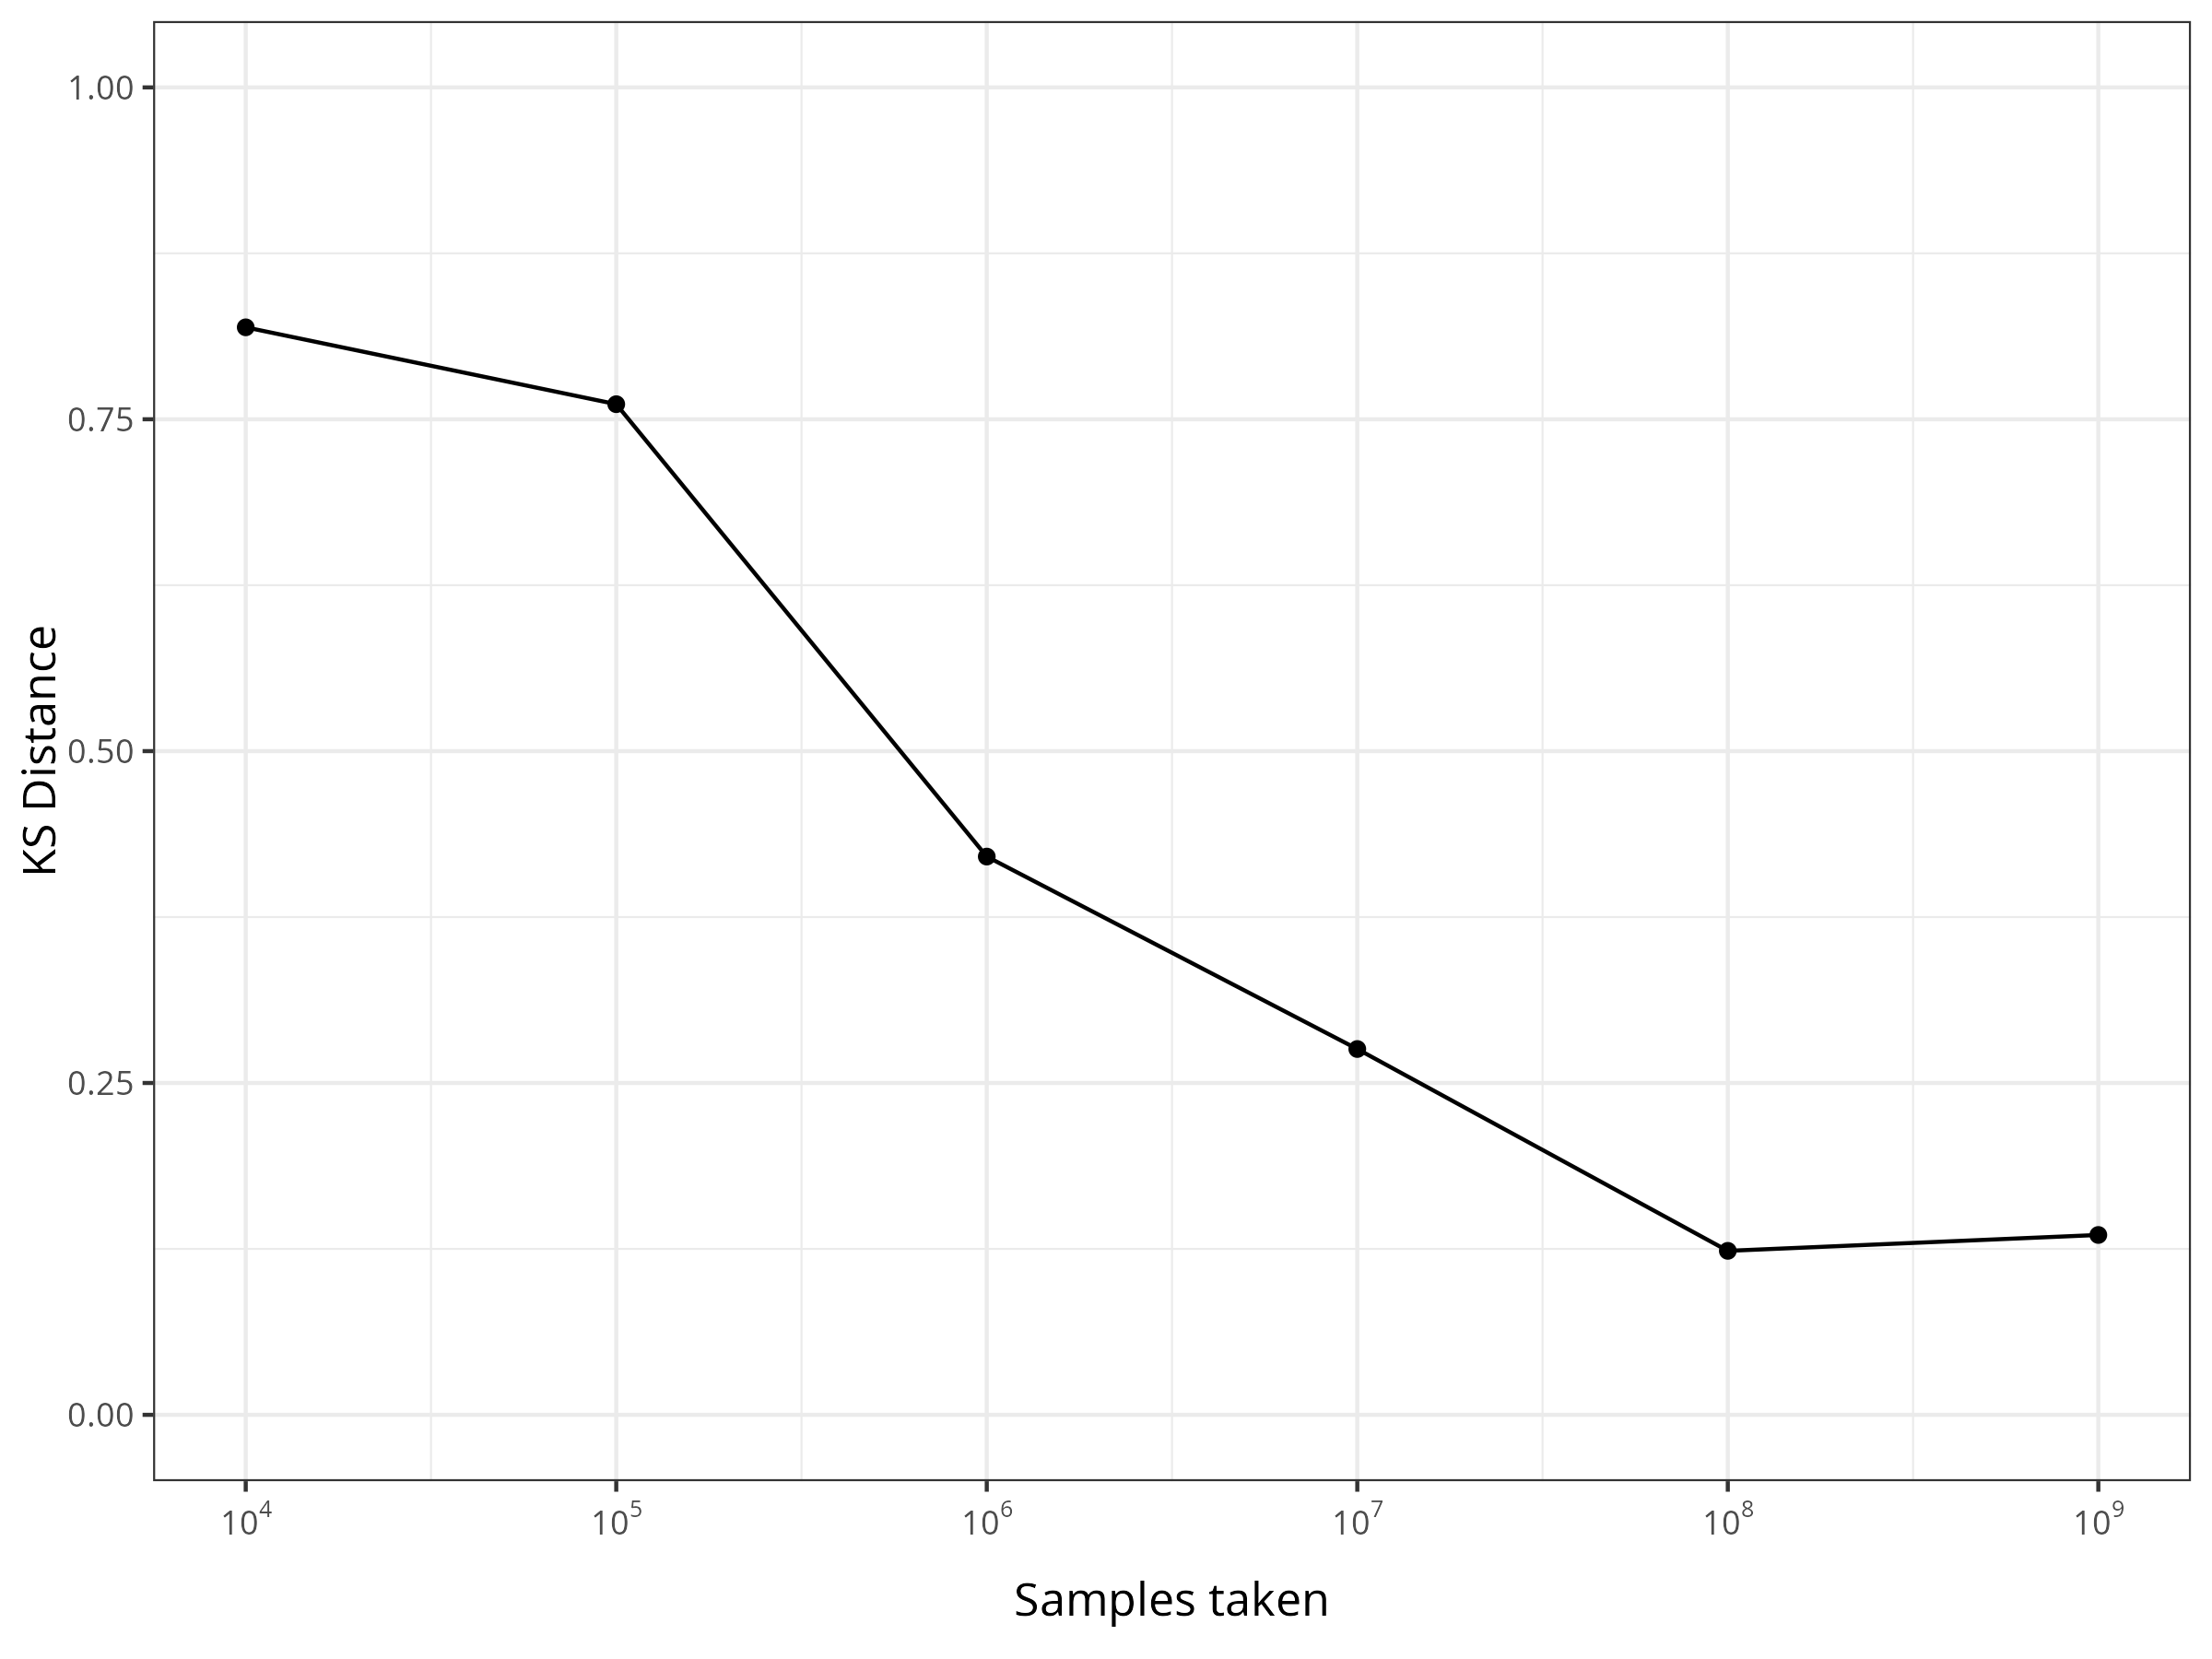
\includegraphics[width=\textwidth]{figures/ks/marsaglia.png}
        \caption{Condensed Table Lookup}
    \end{subfigure}
    \hfill
    \begin{subfigure}{0.46\textwidth}
        \centering
        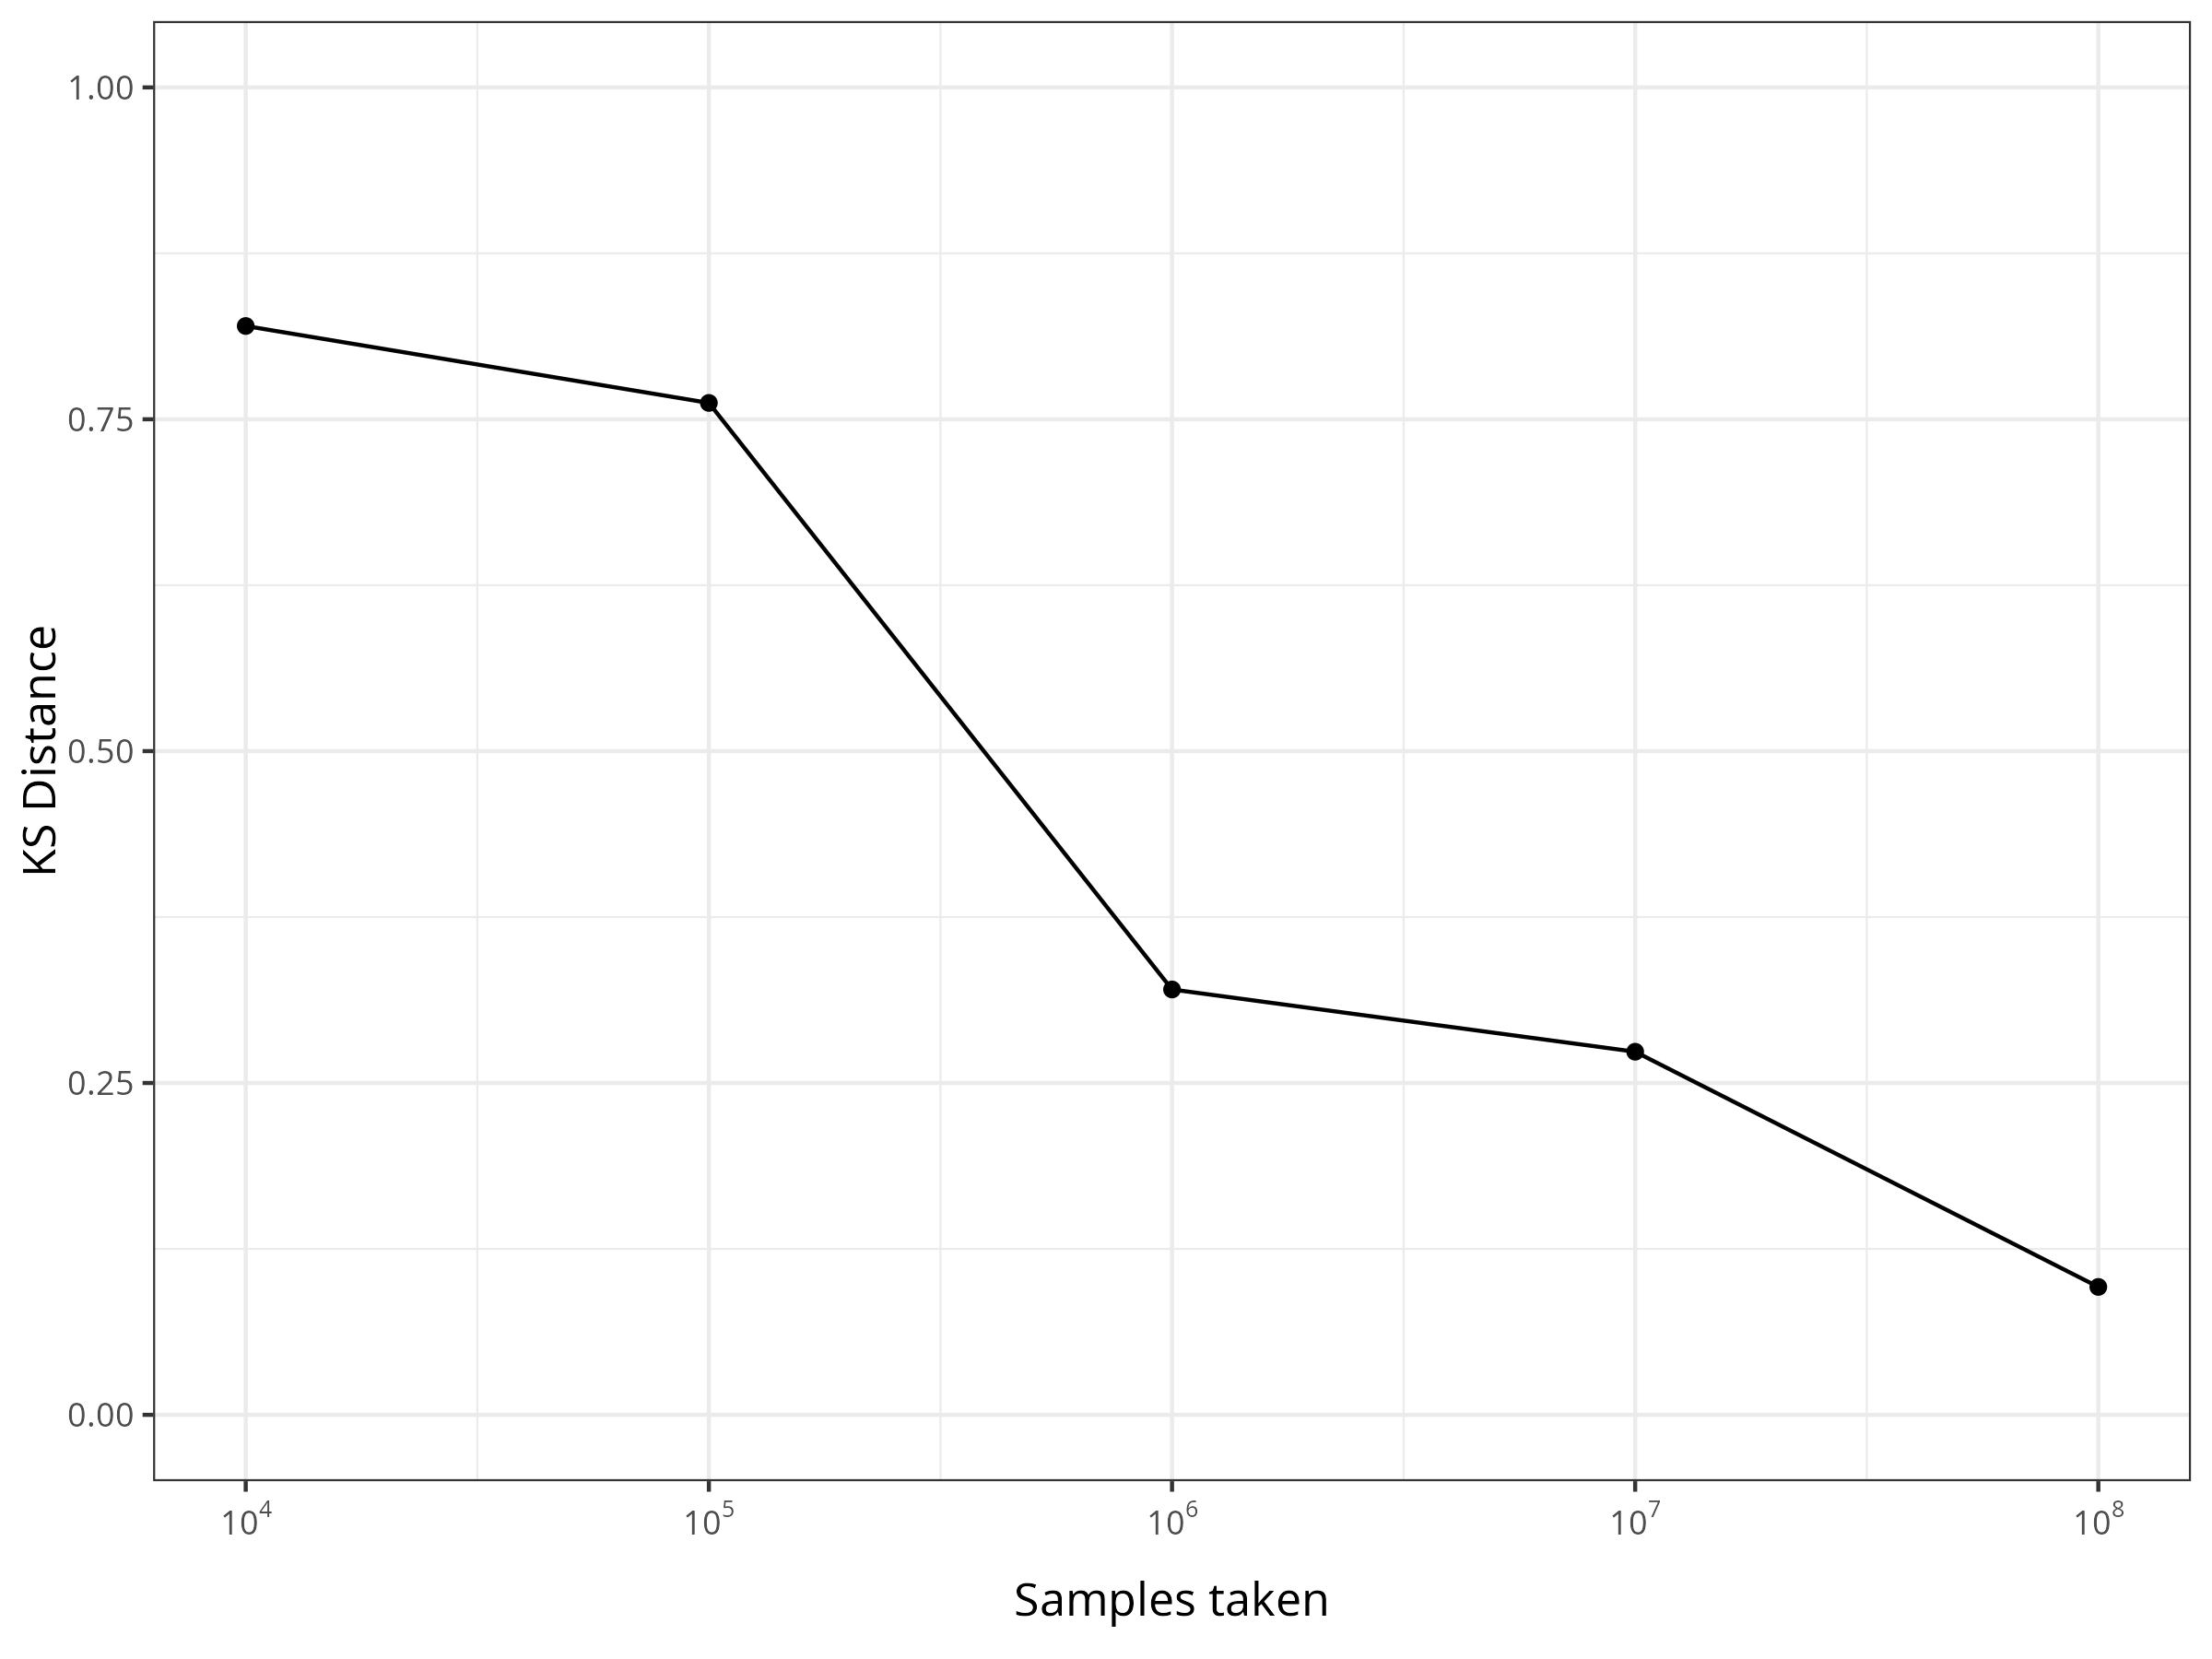
\includegraphics[width=\textwidth]{figures/ks/rejection.png}
        \caption{Rejection Sampling}
    \end{subfigure}

    \caption{Kolmogorov-Smirnov test results for the different samplers.}
    \label{fig:ks_graphs}
\end{figure}

\begin{figure}[t]
    % First row
    \centering
    \begin{subfigure}{0.46\textwidth}
        \centering
        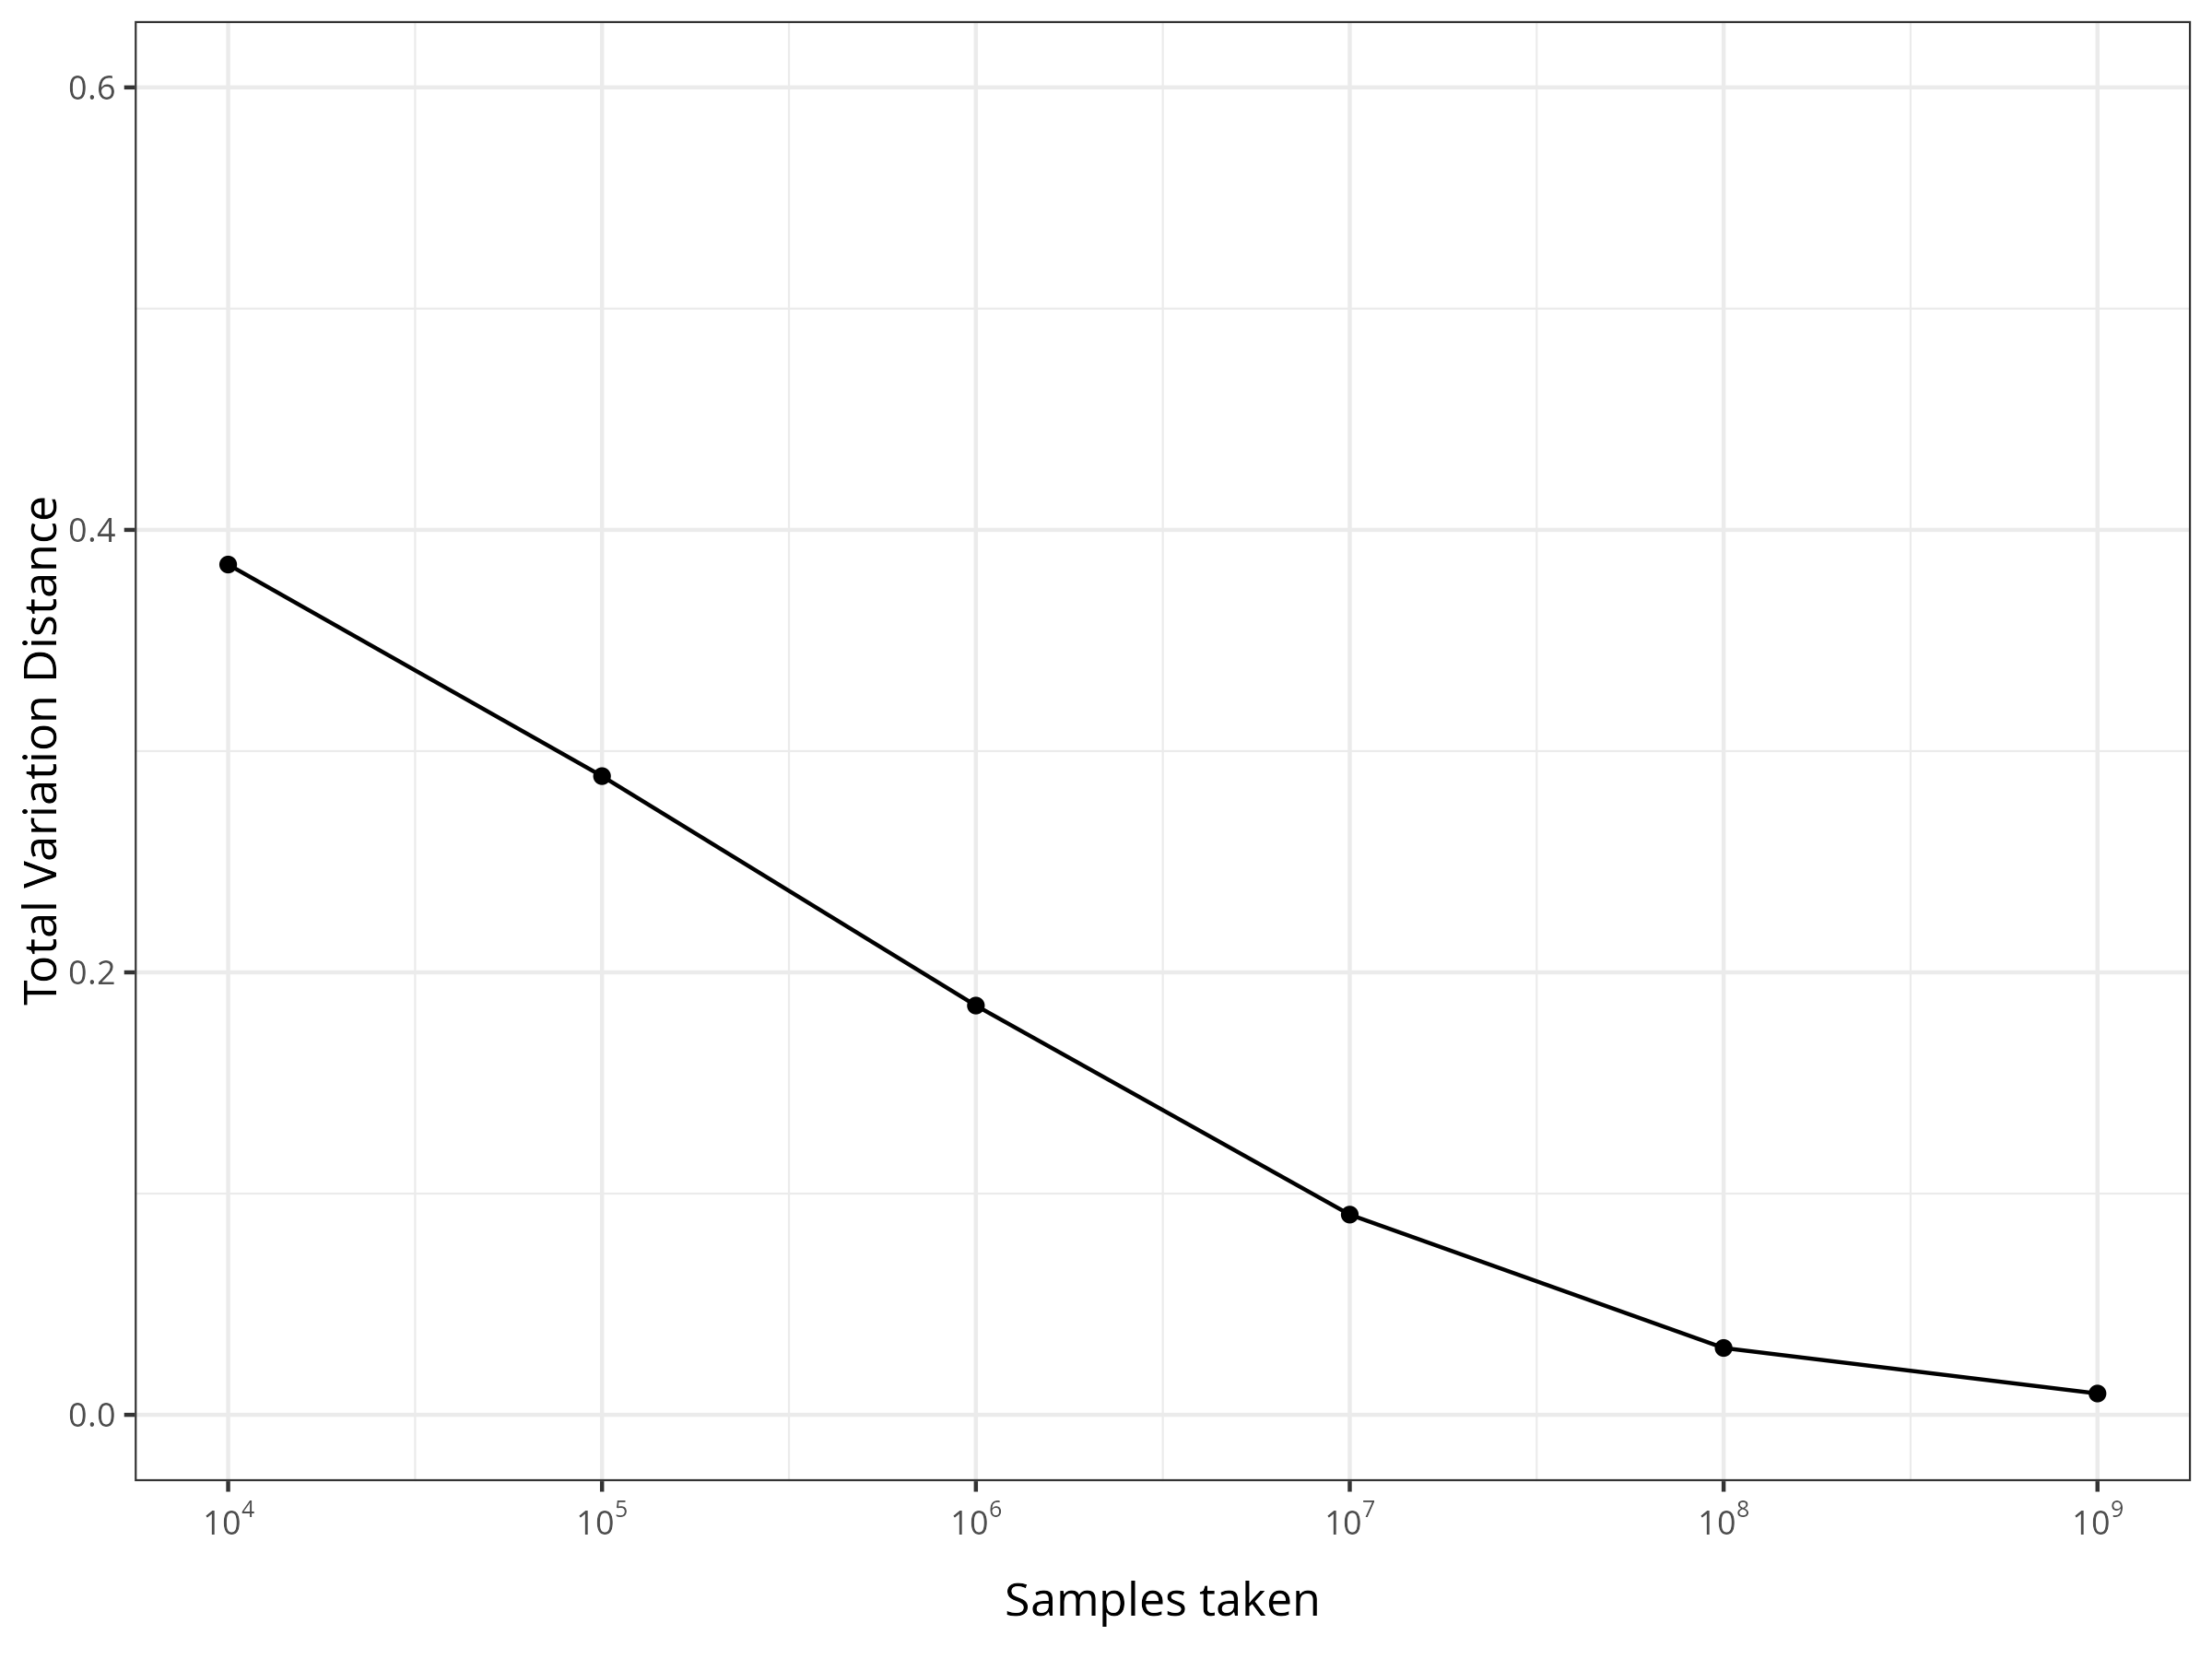
\includegraphics[width=\textwidth]{figures/tvd/apache.png}
        \caption{Rejection-Inversion}
    \end{subfigure}
    \hfill
    \begin{subfigure}{0.46\textwidth}
        \centering
        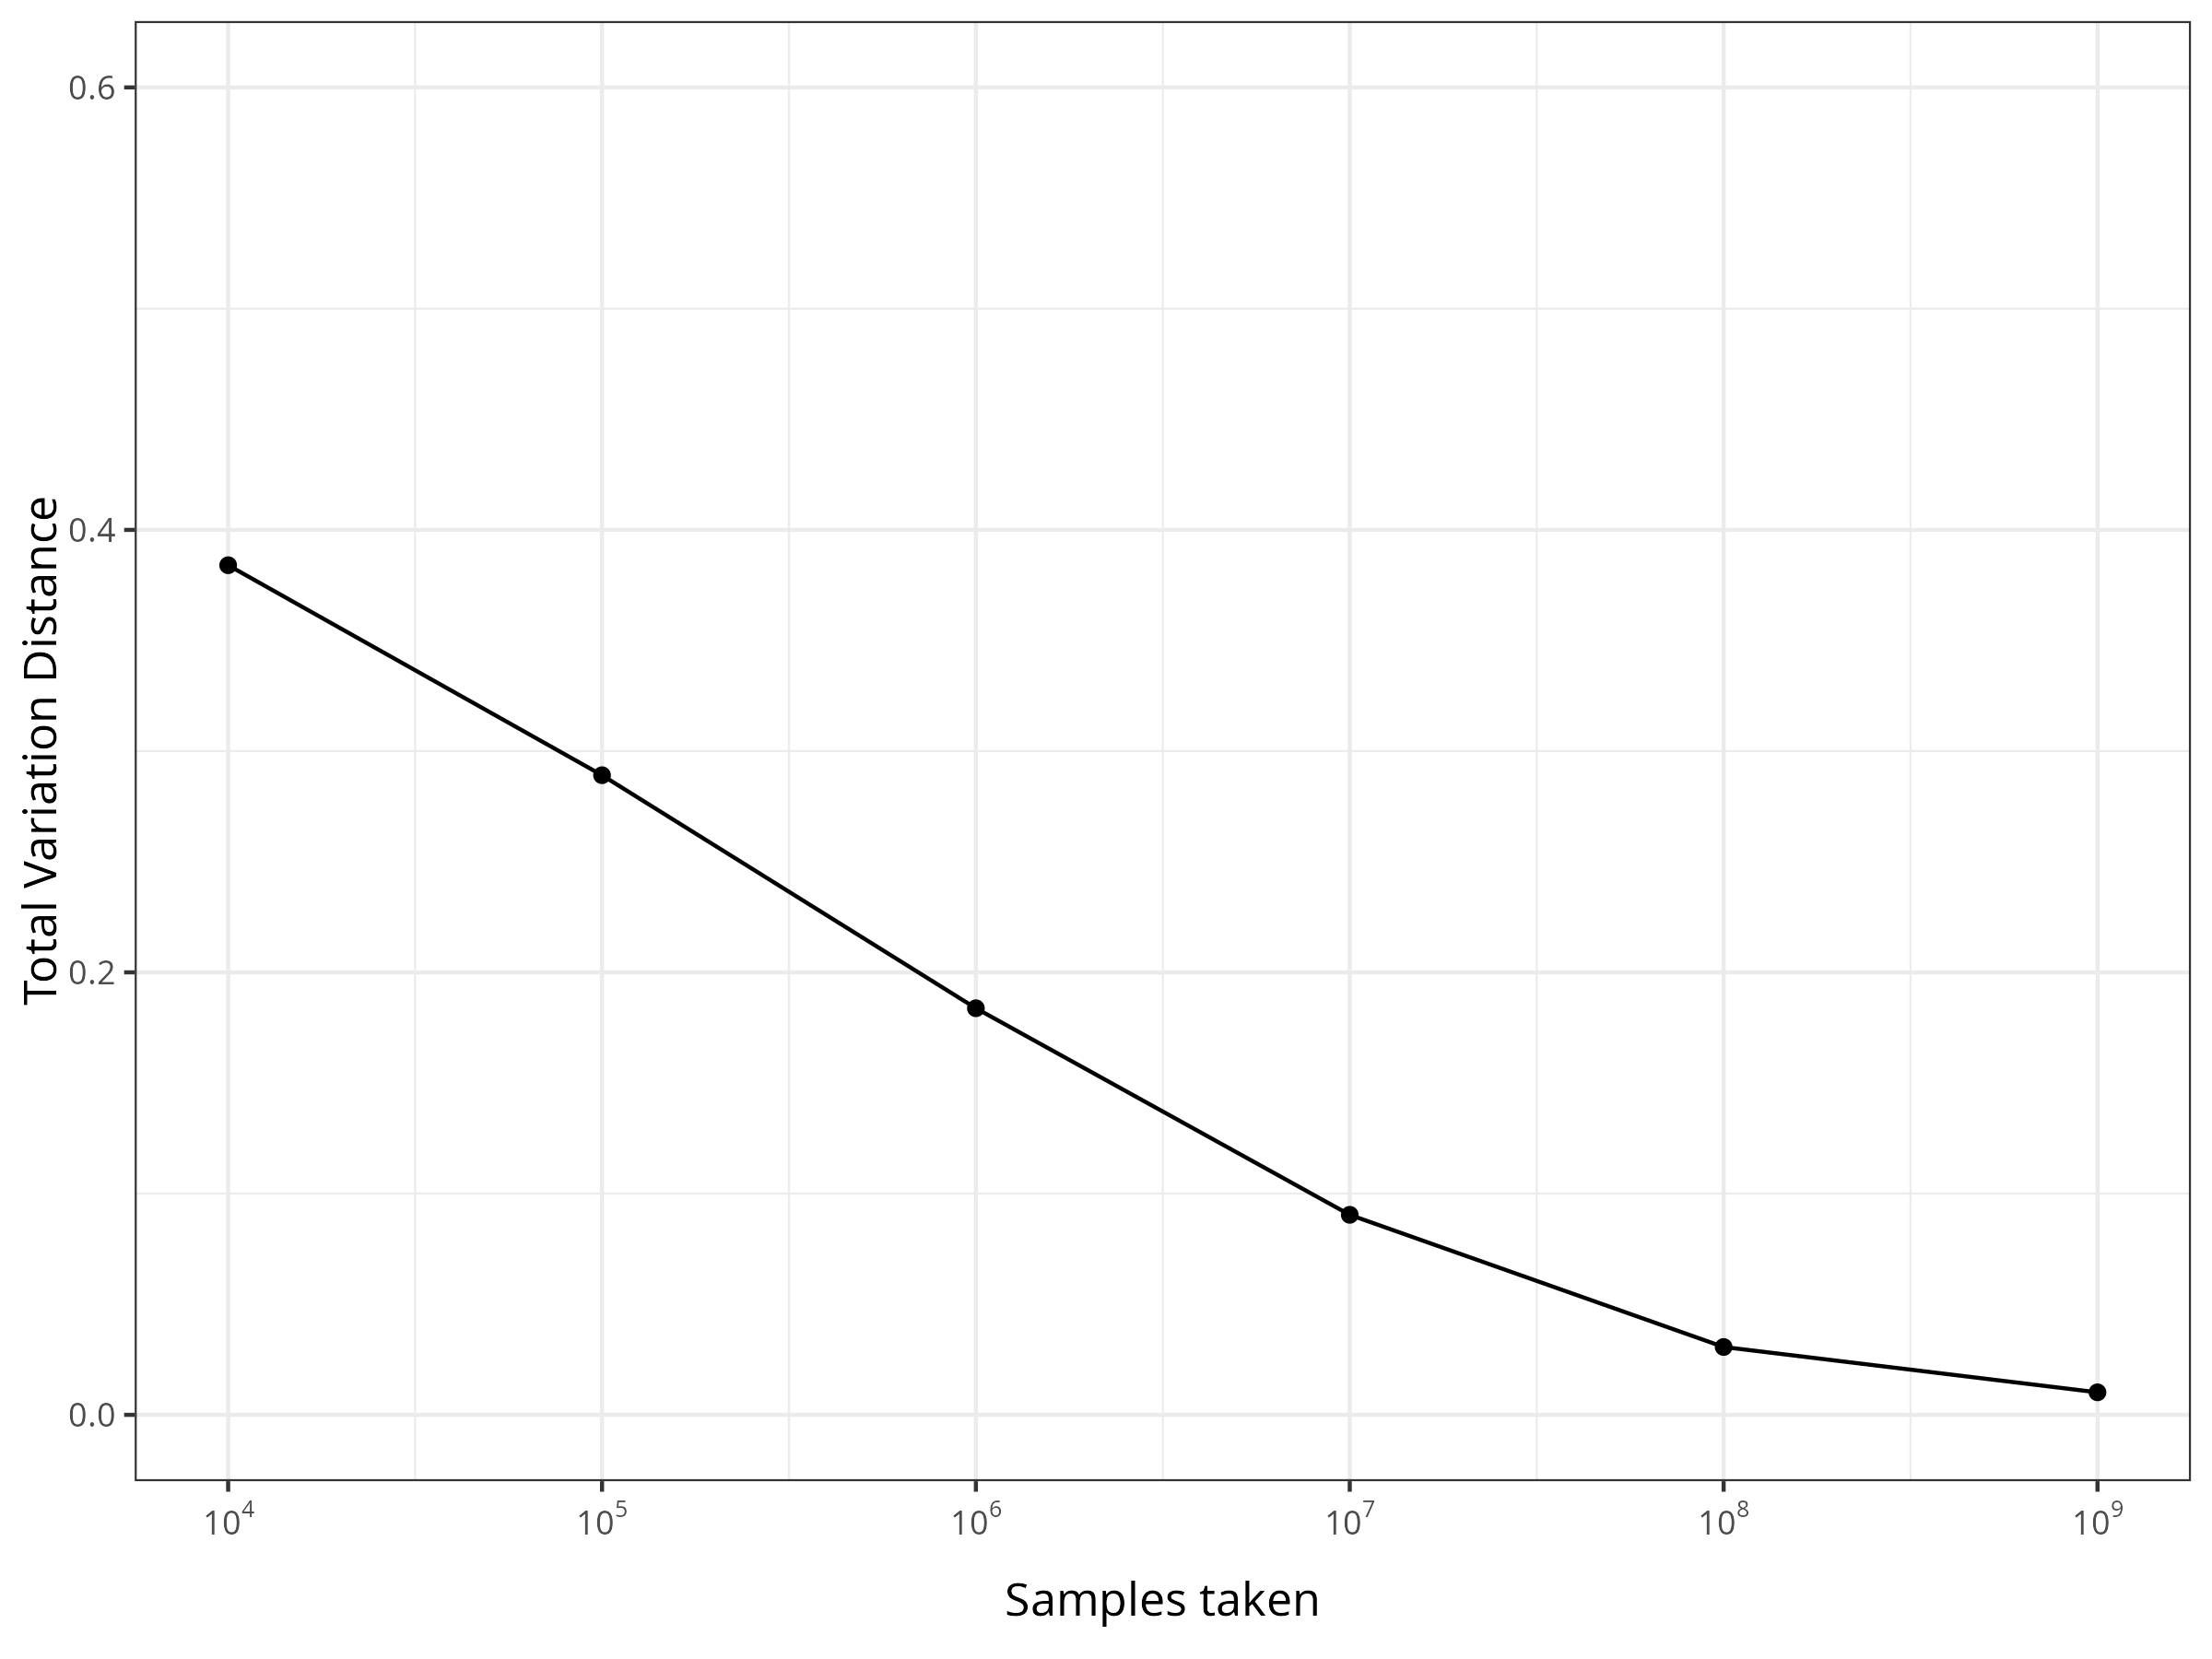
\includegraphics[width=\textwidth]{figures/tvd/ycsb.png}
        \caption{YCSB}
    \end{subfigure}
    
    \vspace{1em}

    % Second row
    \begin{subfigure}{0.46\textwidth}
        \centering
        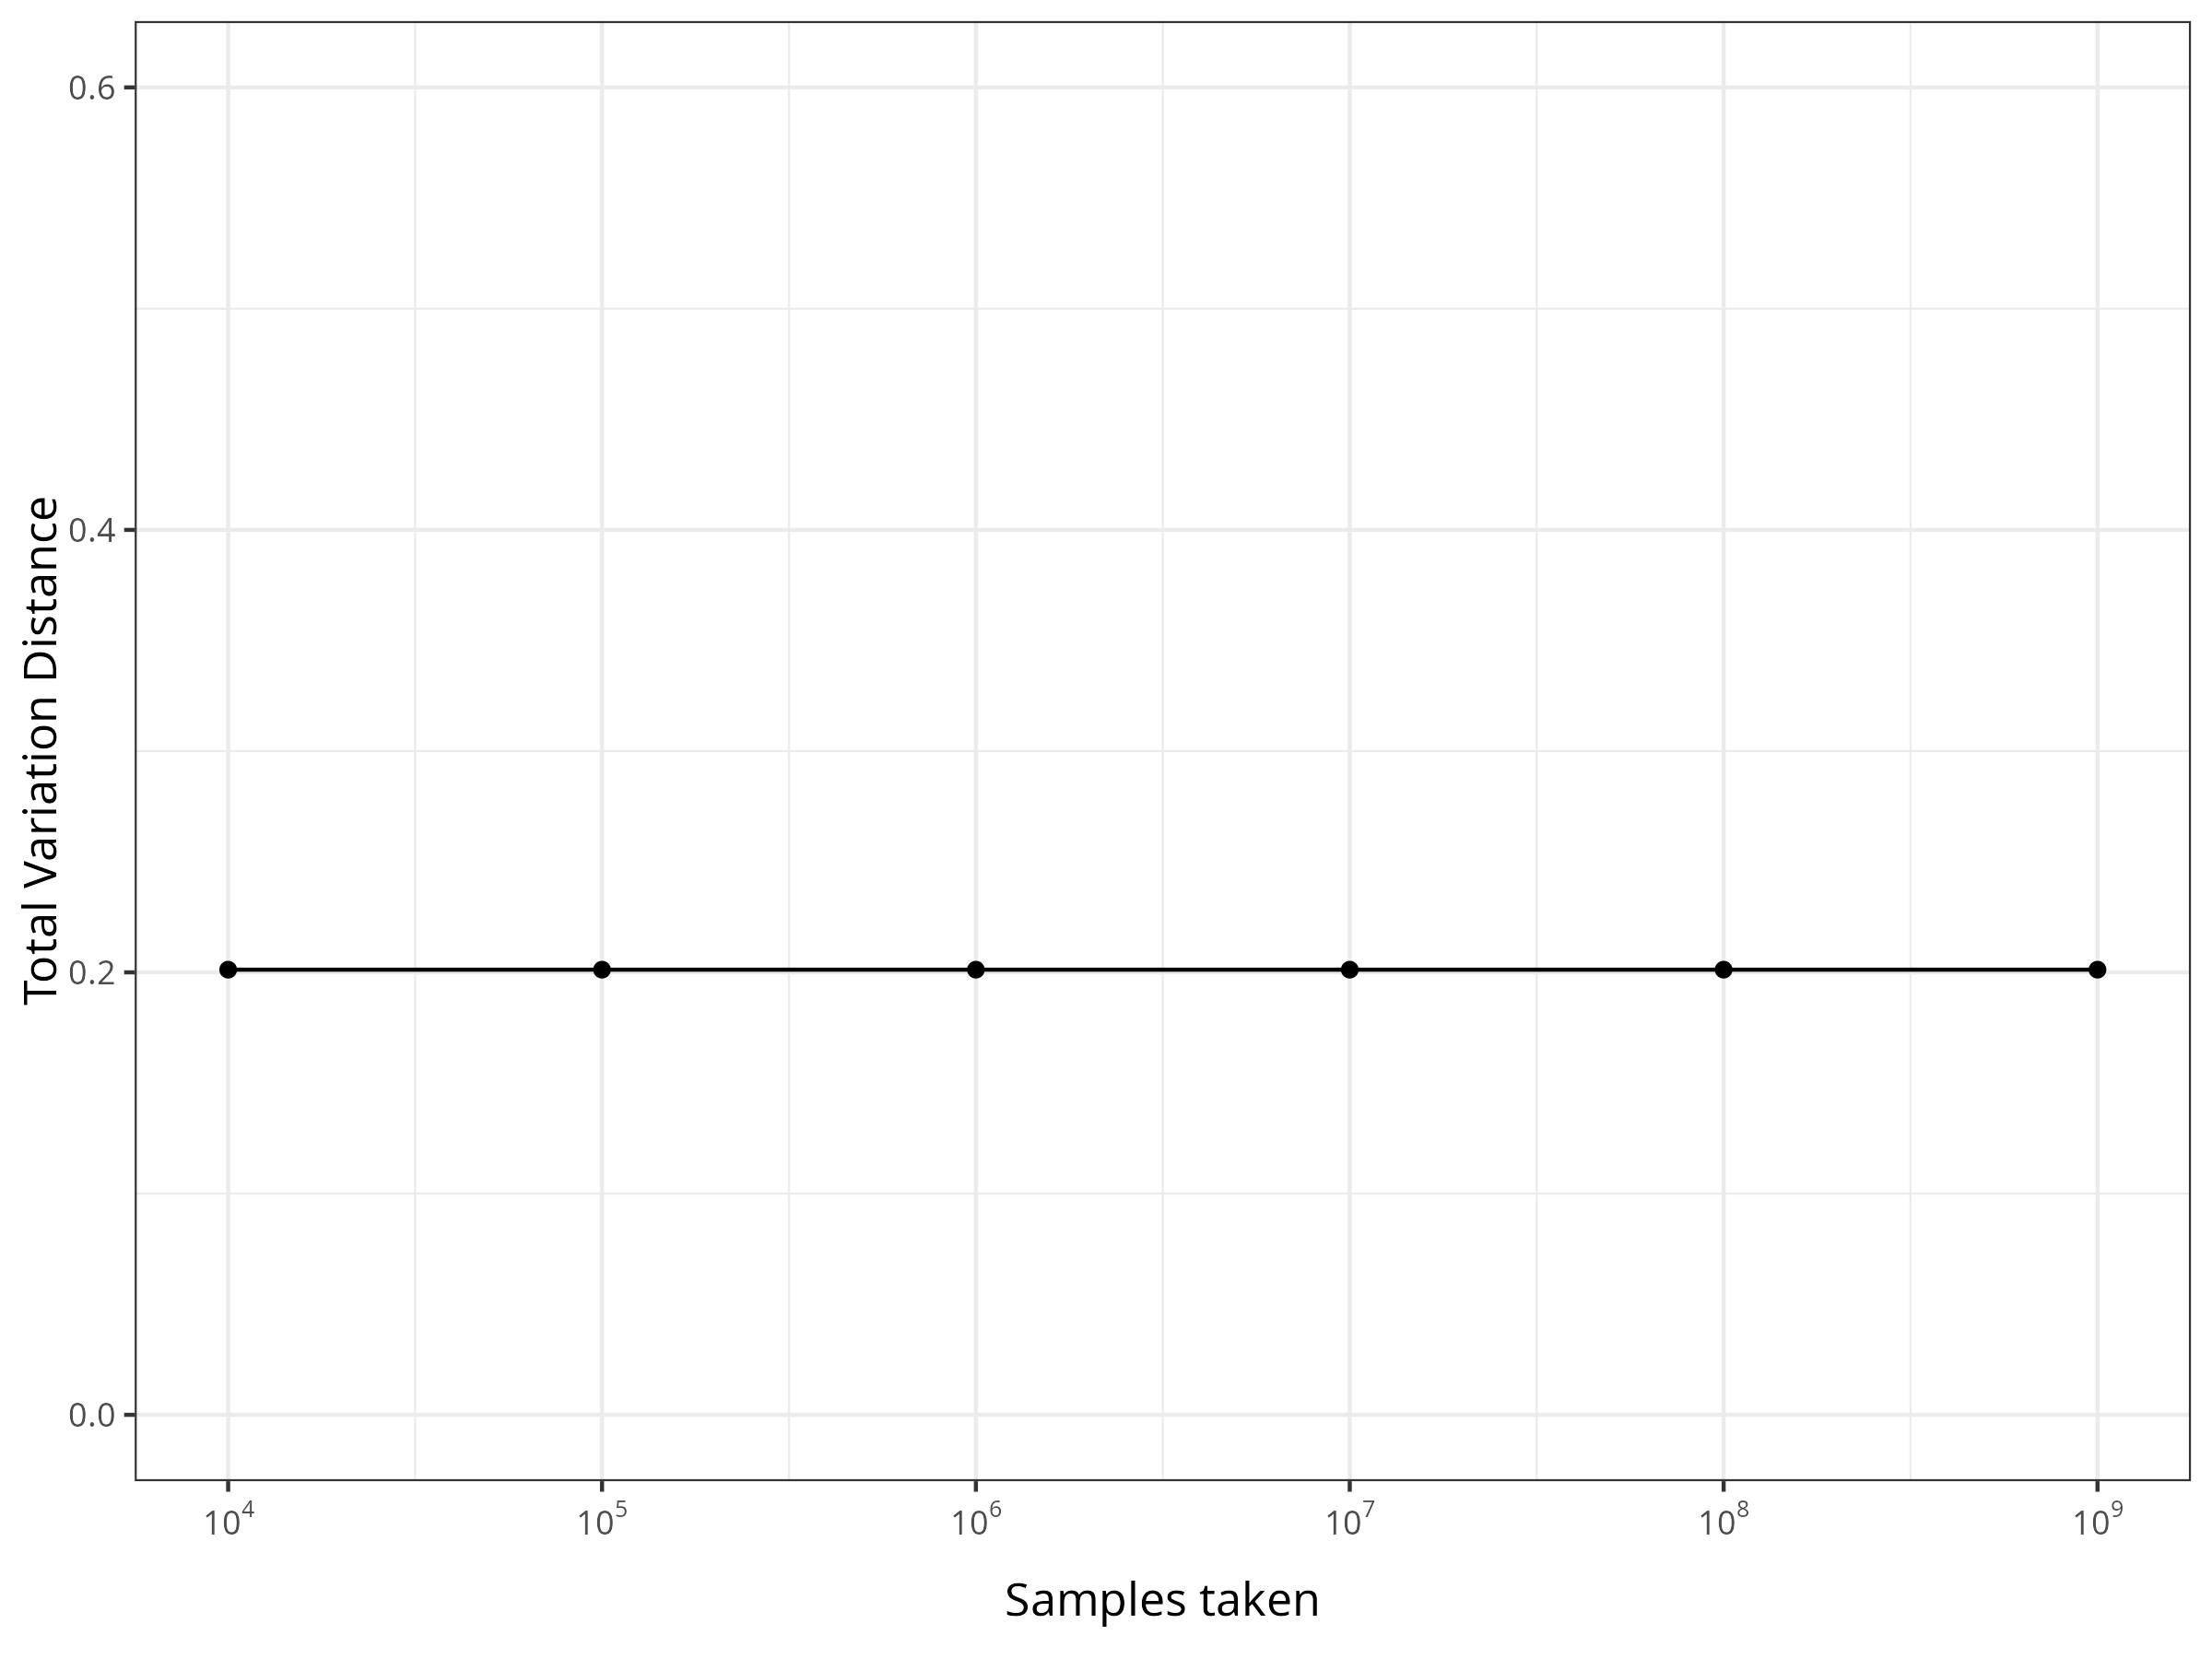
\includegraphics[width=\textwidth]{figures/tvd/fio.png}
        \caption{FIO}
    \end{subfigure}
    \hfill
    \begin{subfigure}{0.46\textwidth}
        \centering
        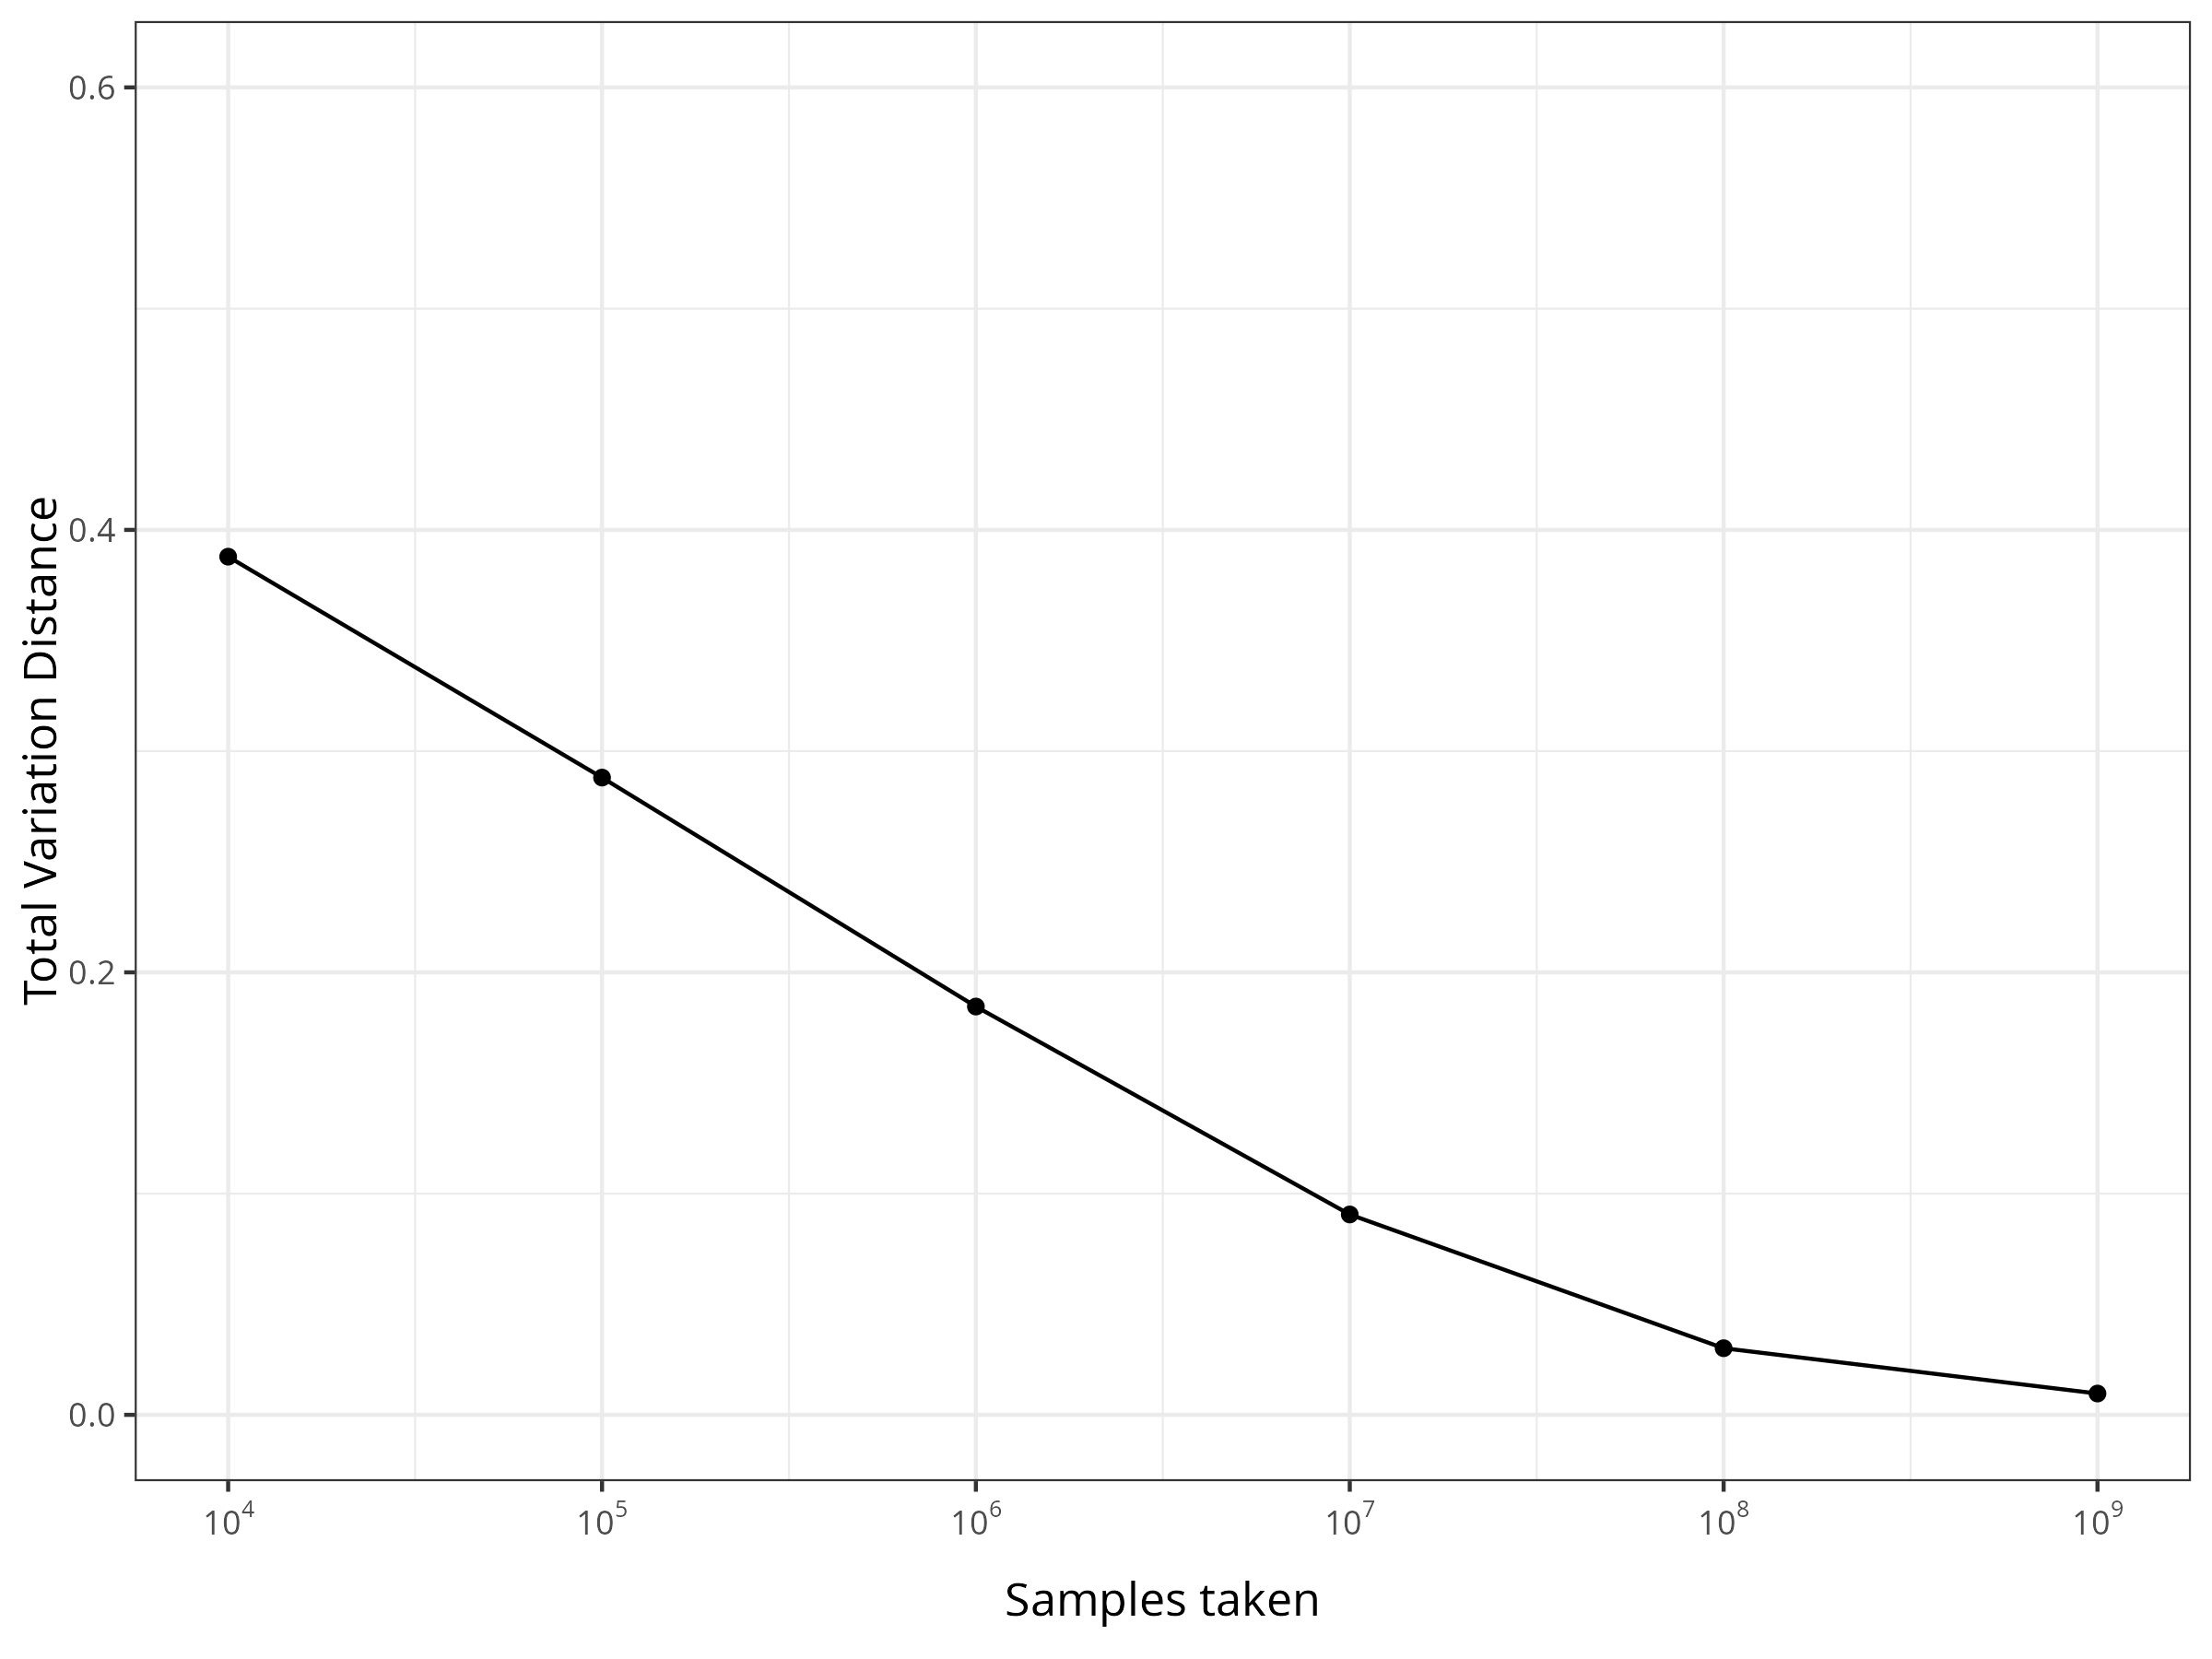
\includegraphics[width=\textwidth]{figures/tvd/sysbench.png}
        \caption{Sysbench}
    \end{subfigure}
    
    \vspace{1em}

    % Third row
    \begin{subfigure}{0.46\textwidth}
        \centering
        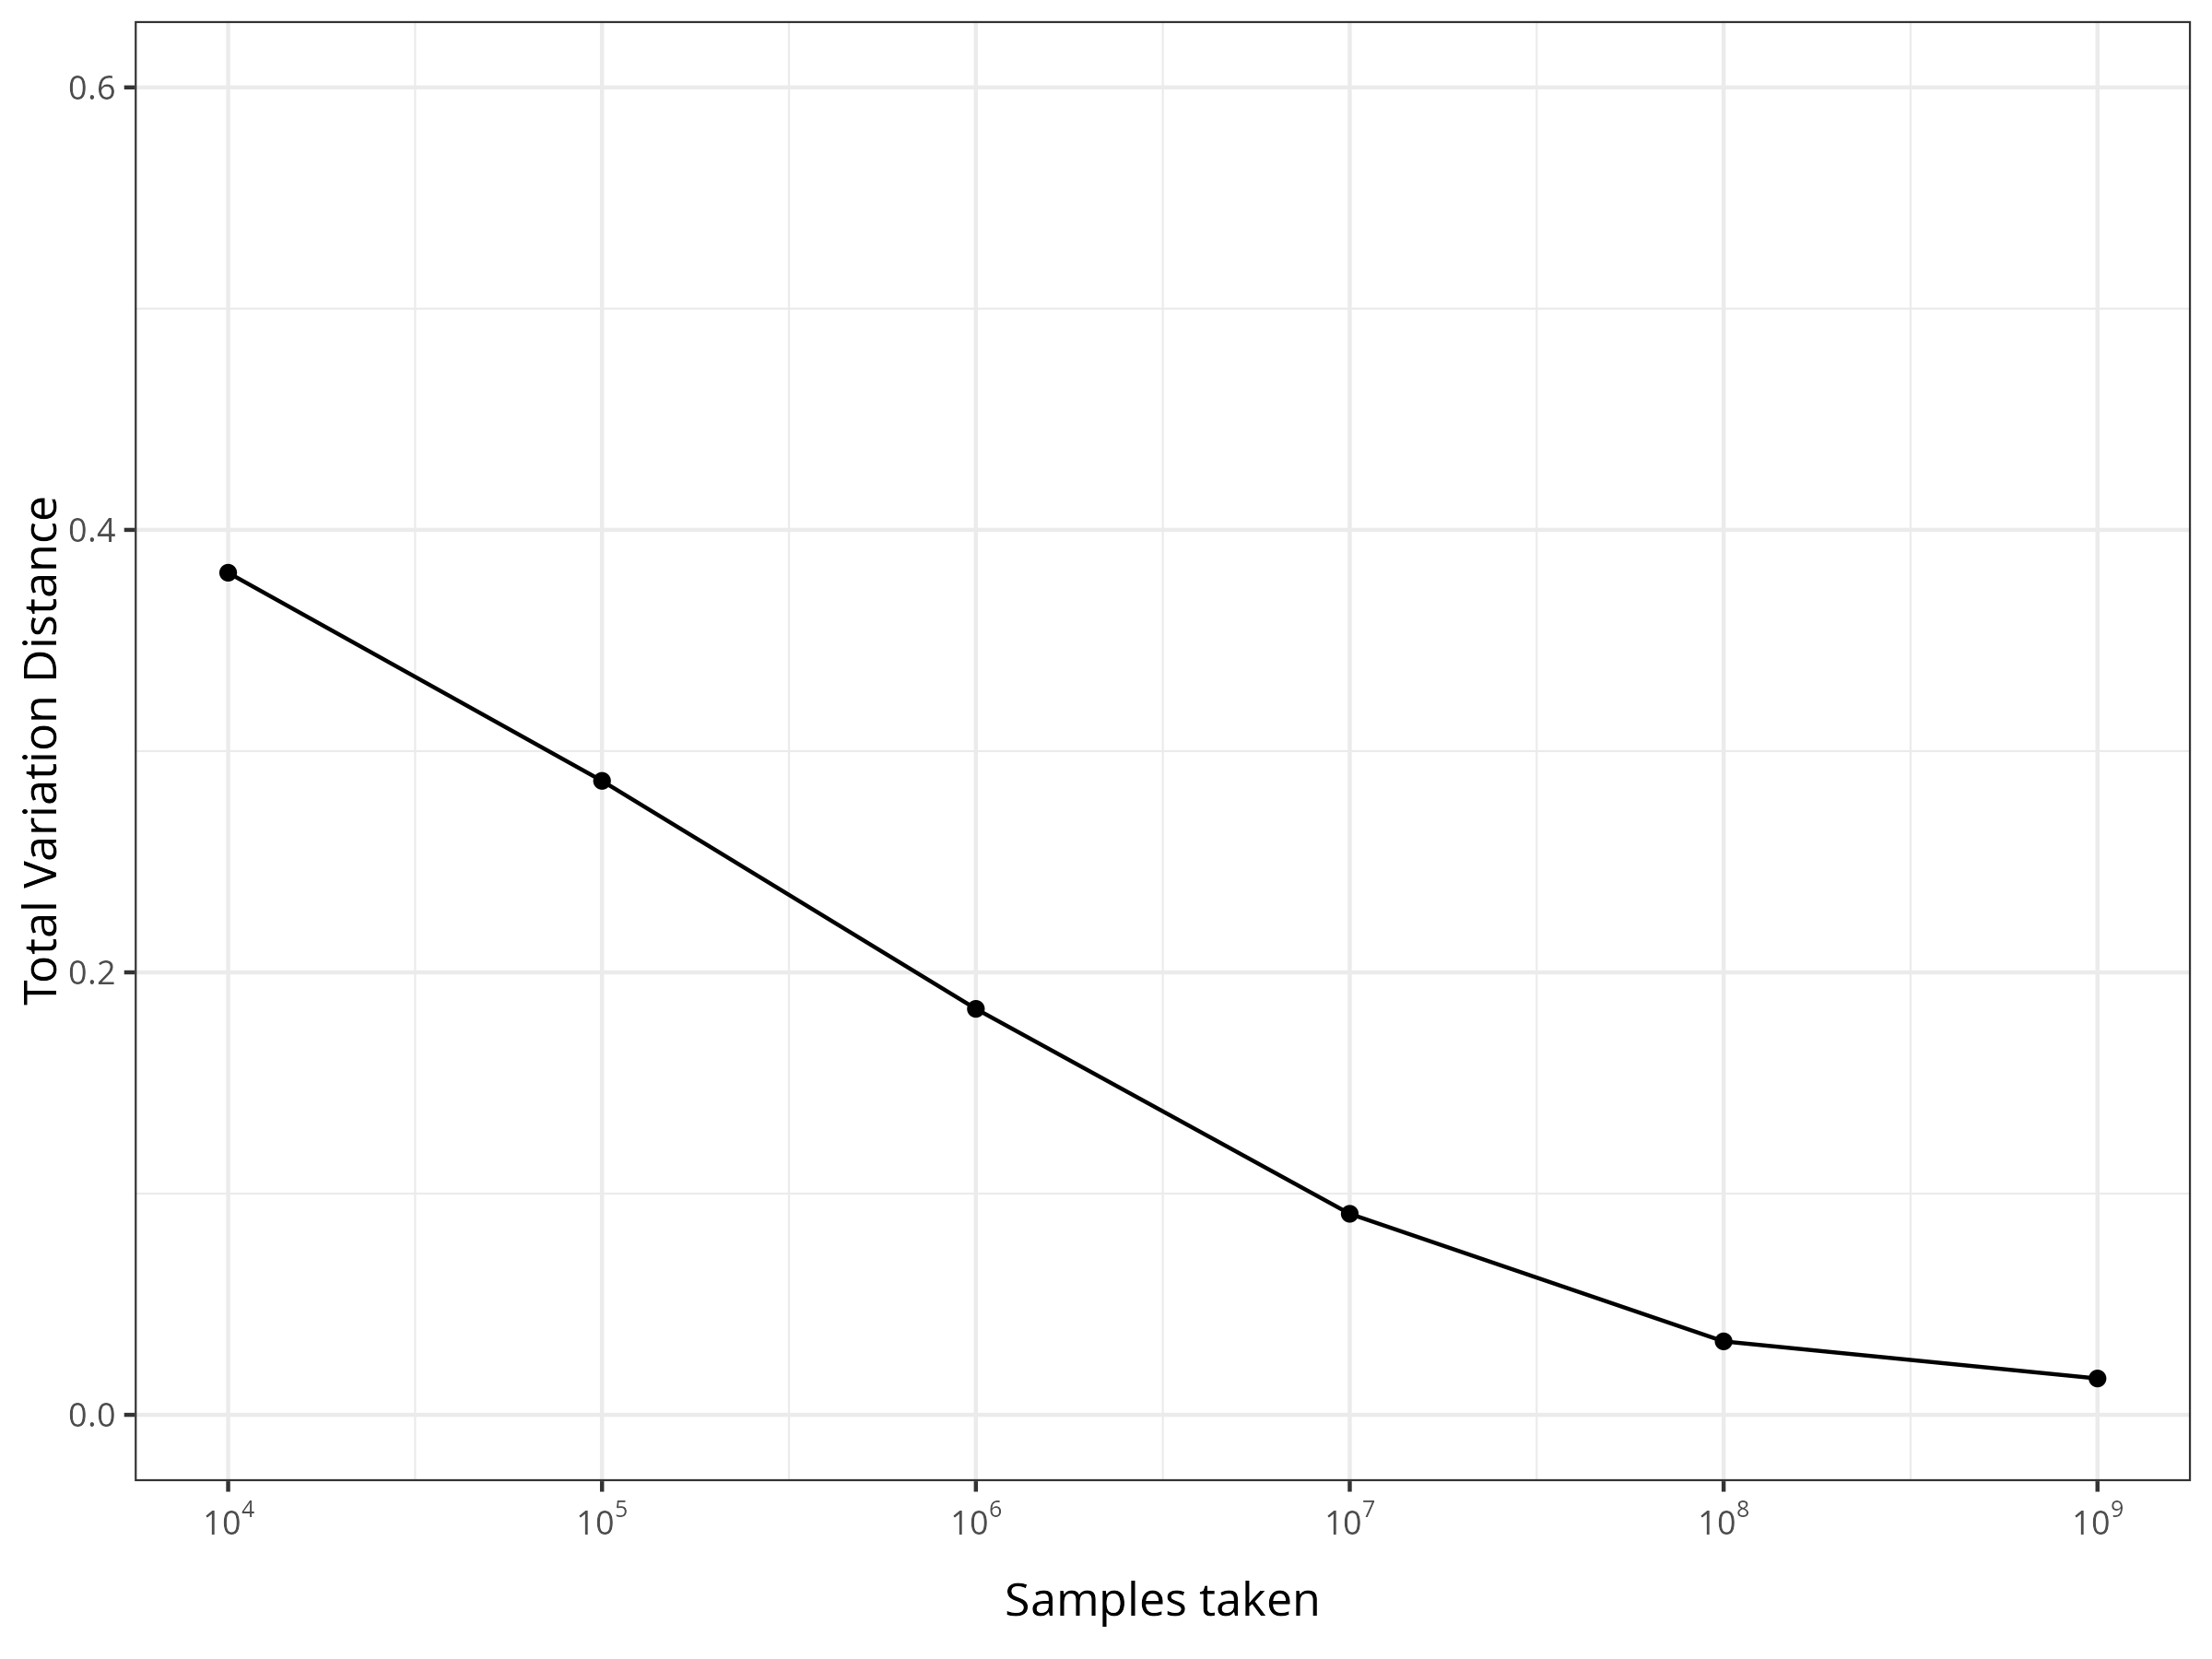
\includegraphics[width=\textwidth]{figures/tvd/marsaglia.png}
        \caption{Condensed Table Lookup}
    \end{subfigure}
    \hfill
    \begin{subfigure}{0.46\textwidth}
        \centering
        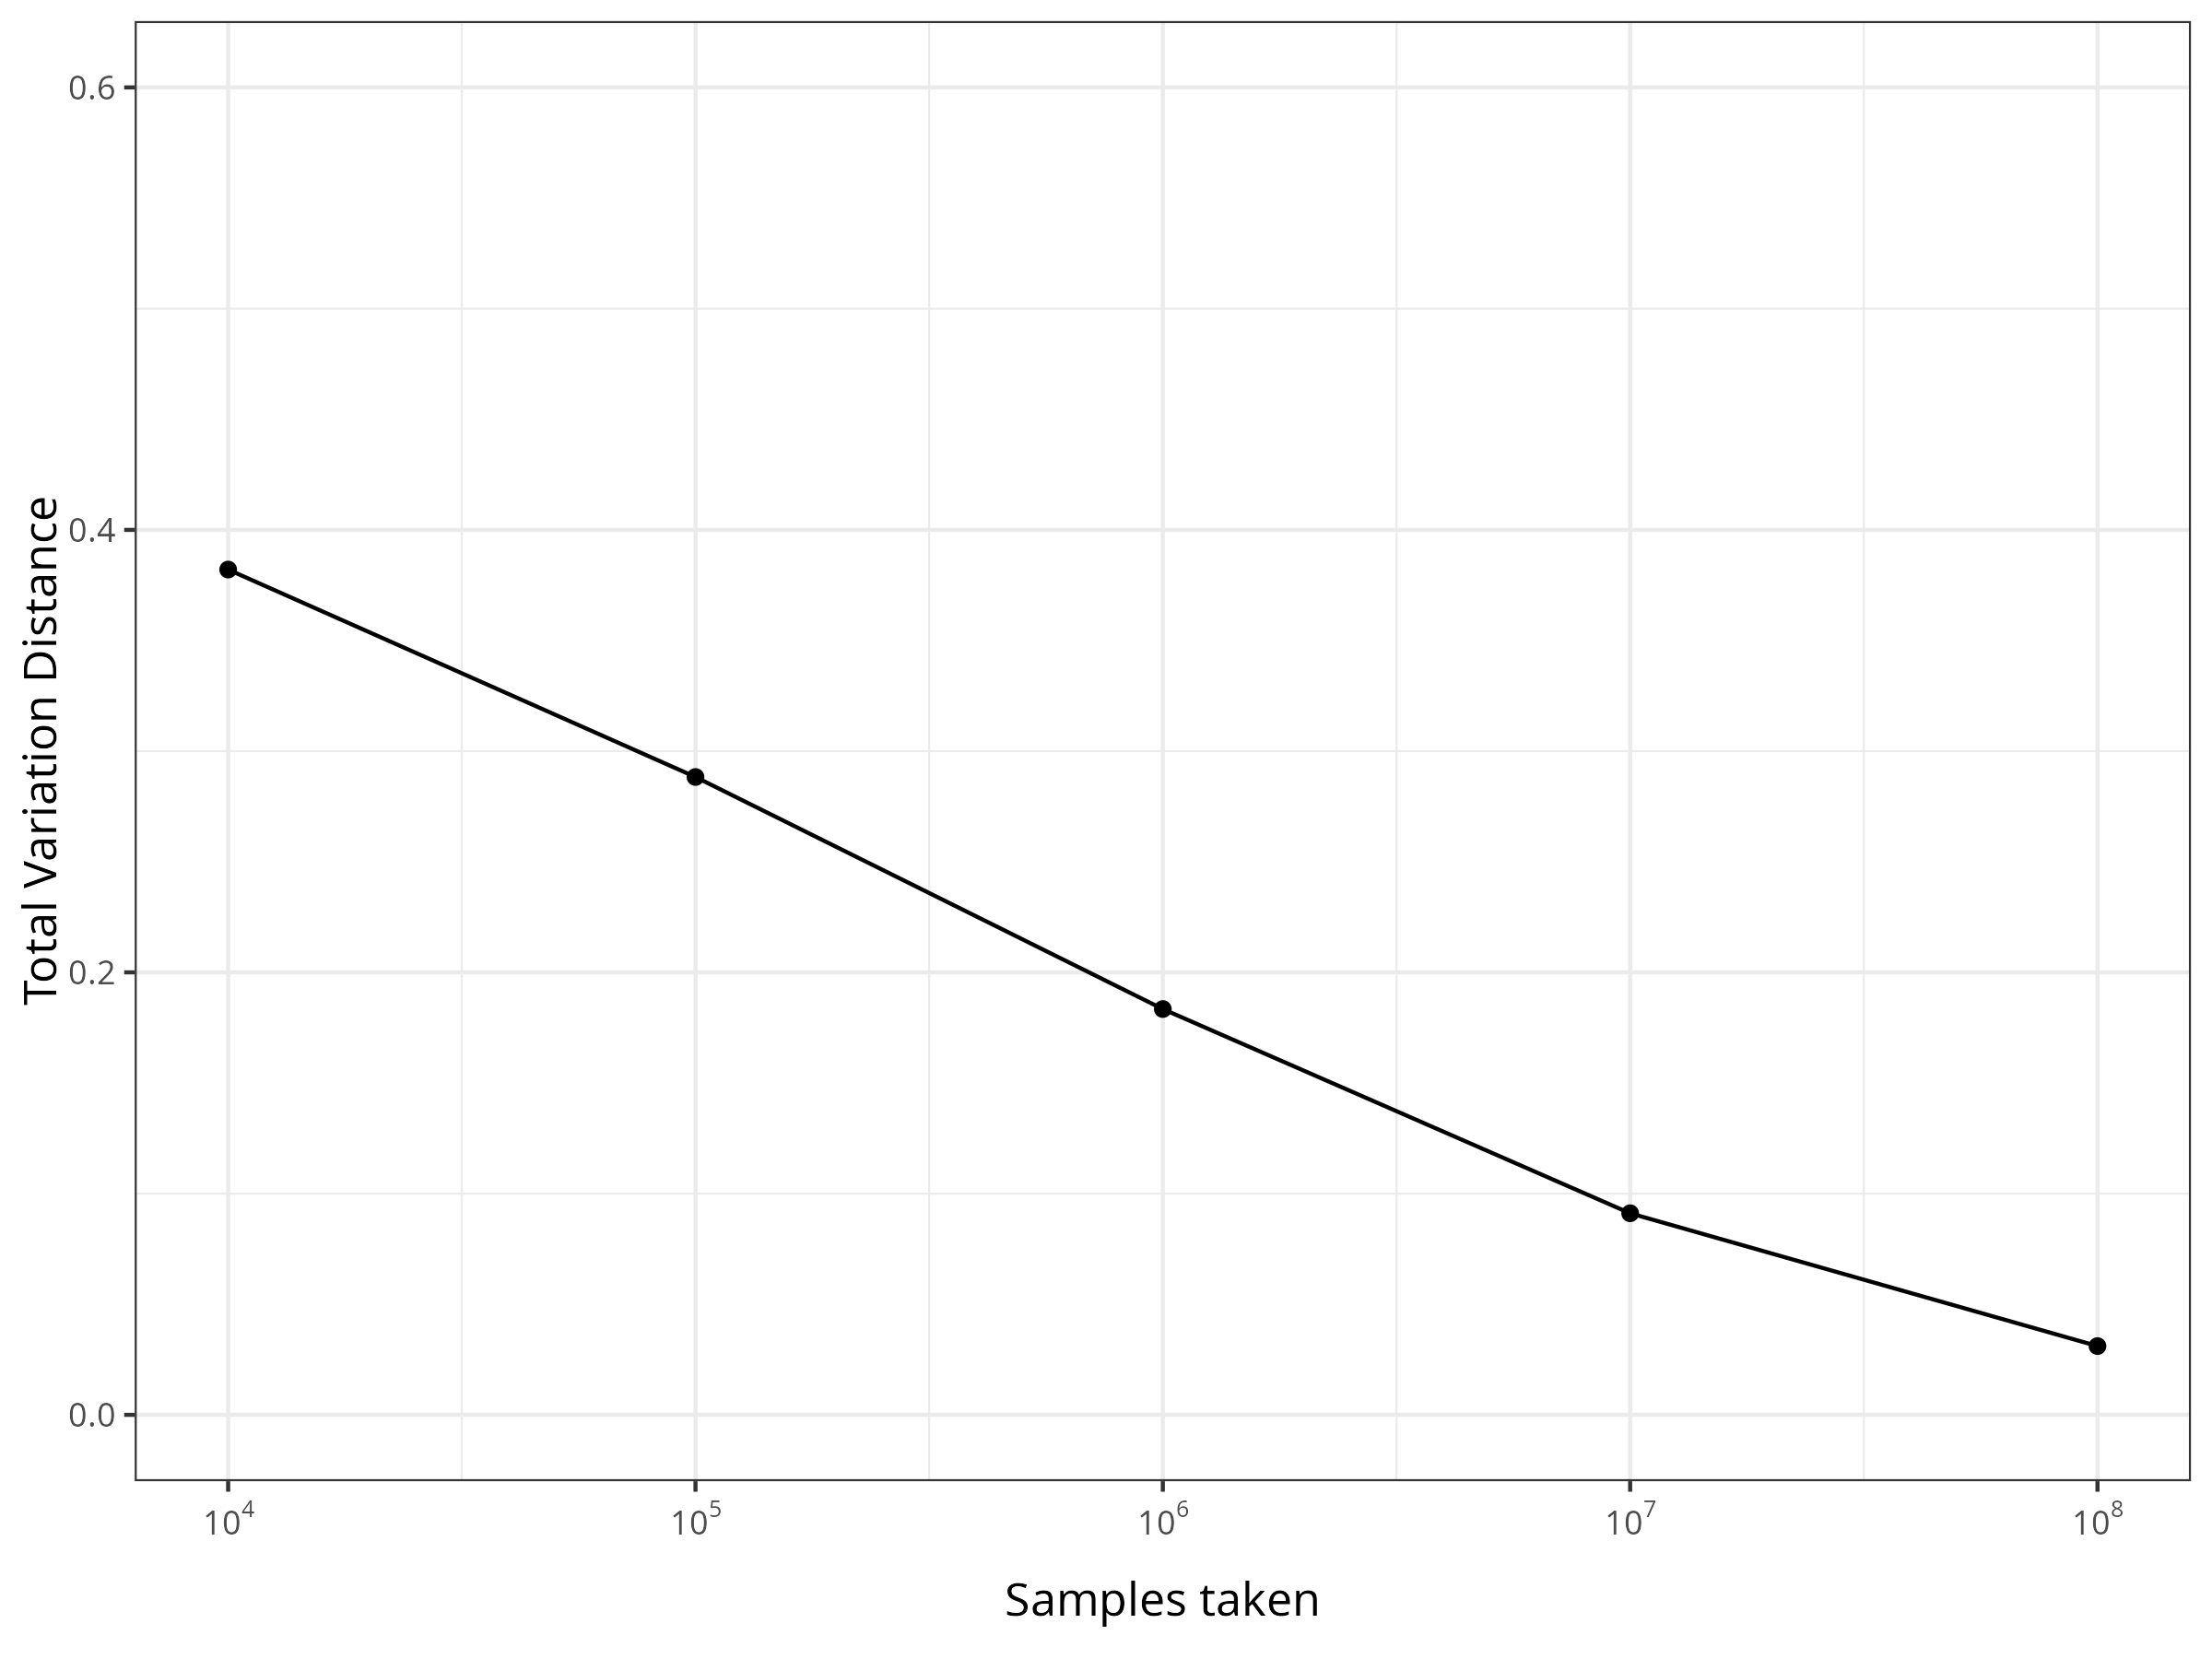
\includegraphics[width=\textwidth]{figures/tvd/rejection.png}
        \caption{Rejection Sampling}
    \end{subfigure}
    
    
    \caption{TVD test results for the different samplers.}
    \label{fig:tvd-graphs}
\end{figure}

\begin{table}[t]
    \centering
    \begin{tabularx}{\linewidth}{|>{\raggedright\arraybackslash}X|>{\raggedright\arraybackslash}X|>{\raggedright\arraybackslash}X|}
        \hline
        \textbf{Sampler} & \textbf{Total Variation Distance} & \textbf{Kolmogorov-Smirnov Statistic} \\
        \hline
        FIO (C) & 0.201 & 0.532 \\
        \hline
        Rejection-Inversion (Java) & 0.00963 & 0.0332 \\
        \hline
        YCSB (Java) & 0.0101 & 0.0338 \\
        \hline
        Sysbench (C) & 0.00963 & 0.0328 \\
        \hline
        Condensed Table Lookup (C++) & 0.0164 & 0.135 \\
        \hline
        Rejection (C++) & 0.031 & 0.0963 \\
        \hline
    \end{tabularx}
    \caption{Accuracy Results for $10^9$ samples}\label{tab:accuracy-results}
\end{table}

\paragraph{Analysis of Accuracy} 
All implementations but FIO and the condensed table lookup present very accurate tendencies when the sample size increases to the scales utilized in benchmarking, which confirm that they are safe to use. It now remains
to explain why both referenced algorithms are not quite as accurate. 

The FIO implementation likely presents systematic deviations from the expected values due to the hashing function used to preprocess the variates, as the variate generation itself follows exactly Jim Gray's pseudocode.
The choice of hashing function falls under the umbrella term "Jenkins Hash Function" (more specifically \textit{lookup3}, see \cite{jenkinsLookup3,HashFunctionHash}) to remap all generated variates before they are counted. Doing this, however,
introduces significant distortions in the distribution, since the aforementioned hash function is not perfect. Furthermore a good hash function should be mostly uniform, the
effect of which can be seen in the graph above as long intervals of constant probability occur. The drops are explained by the fact that eventually the lower-rank values eventually
"differ" enough their bit representation so as to be hashed to a different value. 

The case for the condensed table lookup is more complex. The algorithm is based on a table lookup with precision limited to $2^{30}$, or rather $5 \cdot 10^9$. This means that the algorithm is not able to generate
probabilities which only differ by a factor of $10^{-9}$ will be mapped to the same value. Testing for equality after this mapping yields that the probabilities are $99.9$ pairwise equal among all ranks, which is more
than sufficient to account for the long stretches of constant probability seen in Figure \ref{fig:pmf-graphs}. This effects gets amplified the lower the rank, which explains the ever stretching intervals of constant probability. A possible improvement would be 
to increase the precision of the table lookup, but this would also increase the memory requirements of the algorithm and make it closer to the naive approach.

\section{Evaluating Performance}
As already mentioned, evaluating performance is a tricky business. The main measure of interest is \textit{throughput}, which is the amount of variates generated 
in a time interval. What makes it complicated is controlling for external factors outside of the segment of code being tested. To this end, microbenchmarking is used and
common techniques are applied to avoid pitfalls \cite{AvoidingBenchmarkingPitfalls,beyerBenchmarkingResourceMeasurement2015}.

\subsection{Microbenchmarking}
Microbenchmarking is the process of measuring the performance of small code snippets, usually in the order of microseconds. The main goal is to measure the performance of 
the code in isolation, without the influence of other factors. Since the languages of interest are primarily C++, C and Java (see table \ref{tab:interpreter-versions}), 
the tools used to measure performance will be Google Benchmark \cite{GoogleBenchmarkMicrobenchmark} for C++ and C, and JMH \cite{AvoidingBenchmarkingPitfalls} for Java. 
For C++ and C applications, the following precations will be taken (for instruction on how to accomplish the following, see \cite{BenchmarkingTipsLLVM}):

\vspace{0.3cm}
\fbox{
    \centering
    \parbox{0.8\linewidth}{
        \begin{itemize}
            \item Set specific CPU core for the process
            \item Disable frequency scaling
            \item Disable turbo boost
            \item Limit the available memory to the process
            \item Warm-up runs 
        \end{itemize}
    }
    \label{microbenchmarking-precautions}
}
\vspace{0.3cm}

At last, it's important to define the runs. Since what is going to be measured is throughput, we define the duration of a single run to be 1 second. This will be repeated 30 times
and the average throughput will be calculated. Since the speed is invariant to domain size and distribution parameter, these are kept fixed at $10^8$ and 0.8, respectively.

For the Google Benchmark, the following command will be used to run the benchmarks (for more details on how to use the tool, see \cite{GoogleBenchmarkMicrobenchmark}):
\begin{lstlisting}
    ./benchmark --benchmark_repetitions=30 --benchmark_min_warmup_time=1.0
\end{lstlisting}

As a precaution for the sample generation not be optimized away, the function \verb|benchmark::DoNotOptimize| on the results of the computation was used. Similarly for the JMH (more details on \cite{AvoidingBenchmarkingPitfalls,jenkovJMHJavaMicrobenchmark}):
\begin{lstlisting}
    java -jar target/benchmarks.jar -bm thrpt -wi 10 -i 30 -f 1 -r 1
\end{lstlisting}

The results depende heavily on which JVM is used, but some common patterns exist to avoid making code be optimized away:              
\begin{itemize}
    \item Use the \verb|Blackhole| object to consume the results of the computation
    \item Use the \verb|@CompilerControl| annotation to avoid inlining
    \item Use the @\verb|State| annotation to avoid dead code elimination
\end{itemize}

\begin{table}[t]
    \centering
    \begin{tabular}{|c|c|c|c|}
        \hline
        \textbf{Sampler} & \textbf{Average Throughput (M/s)} & \textbf{Standard Deviation} \\
        \hline
        FIO (C) & 26.2 & 0.01 \\
        \hline
        Rejection-Inversion (Java) & 27.4 & 0.07 \\
        \hline
        YCSB (Java) & 29.9 & 0.14 \\
        \hline
        Sysbench (C) & 43.6 & 0.15 \\
        \hline
        Condensed Table Lookup (C++) & 45.2 & 0.06 \\
        \hline
        Rejection (C++) & 28.1 & 0.3 \\
        \hline
    \end{tabular}
    \caption{Microbenchmarking Results}\label{tab:microbenchmarking-results}
\end{table}

From the table \ref{tab:microbenchmarking-results}, we can recognize that the Condensed Table Lookup sampler is the fastest, which is to be expected given that the main operation is a table lookup,
while the cost gets offloaded to the initialization. The Sysbench sampler is the second fastest, which is expected given the overhead of the JVM.
But to further investigate why this difference is present, arun with a profiler is required. Running \verb|perf|\cite{PerfLinuxProfilinga} 
along with the JMH tool yields the following results for YCSB and Rejection-Inversion (Java). Only relevant lines are presented.

\begin{perfbox}{Rejection-Inversion (Java)}
\ttfamily
Baseline: 565.140.532.065 instructions 4,33  insn per cycle \\  
Sampler: 204.065.670.512  instructions  1,56 insn per cycle   \\
Sampler: 11.310.090  L1-dcache-load-misses  0,02\% of all L1-dcache accesses 
\end{perfbox}

\begin{perfbox}{YCSB}
\ttfamily
Baseline: 578.884.719.478 instructions 4,43 insn per cycle \\         
Sampler : 392.403.334.414  instructions 2,92  insn per cycle \\
Sampler: 339.375.866 L1-dcache-load-misses  0,43 \% of all L1-dcache accesses \\ 
Sampler: 789.273 L1-icache-load-misses 0,30\% of all L1-icache accesses 
\end{perfbox}

Given that both the baseline and the actual sample routine have similarly high IPC and low number of data and instruction cache misses, the lower throughput in Java is likely 
not caused by an inefficient implementatation, but rather by the overhead inherent to the JVM runtime, such as garbage collection, memory management and JIT compilation. These aspects
won't be explored further, which limits a rigorous conclusion. Nonetheless this points towards the JVM being responsible for the difference in performance.

\section{Overall Evaluation}

The results of the evaluation show that the Rejection-Inversion and Sysbench implementations are the most accurate and performant, closely followed by YCSB. 
The condensed lookup table is the fastest, but also less accurate. While currently the problems explored in the \textit{frequency ratio graphs} exclude it from further consideration, it could be improved by increasing the precision of the table lookup so as to make it competitive
with the other implementations. The FIO implementation is the least accurate and the slowest, which makes it unsuitable for further use. Lastly, the rejection algorithm is among the slowest and also not particularly accurate, which
excludes it from any further consideration. All in all, YCSB and Sysbench are the most viable choices for further use, as they are both accurate and performant and cover the use cases of database and file system benchmarks respectively.


`'
\chapter{Future Work}\label{chap:future-work}

This thesis provided a comprehensive overview of existing methods for sampling from a Zipfian distribution in the context of 
database and storage systems research. However, further exploration of the broader field of power-law variate generation could 
uncover additional sampling algorithms that exploit structural properties specific to the Zipfian distribution \cite{powersApplicationsExplanationsZipfs1998a}. 

Another promising avenue for future research lies in table-based methods. Historically, these were often dismissed due 
to memory limitations \cite{hormannRejectioninversionGenerateVariates1996}. Yet, this thesis has demonstrated their viability 
in modern environments, despite falling short of delivering a competitive implementation.

Extending the evaluation framework to include other commonly used distributions - such as normal or Pareto - could also prove valuable, 
as these access patterns are frequently employed in performance benchmarking \cite{cooperBenchmarkingCloudServing2010}. 

Additionally, this work identified a gap in the literature concerning the use of error metrics for evaluating the accuracy of non-uniform variate generators. 
While it is well-known that digital computation introduces inaccuracies in such processes \cite{radicchiUnderestimatingExtremeEvents2014,leydoldErrorDetectionNonUniforma,monahanAccuracyRandomNumber1985},
there is little consensus on which metrics are most appropriate. As a result, the metrics chosen in this thesis prioritized interpretability, but future research could benefit from a more rigorous framework for error evaluation.
\chapter{Conclusion}\label{chapter:conclusion}

This thesis investigated the state-of-the-art in discrete variate generation for Zipfian distributions within benchmarking applications used in storage and database systems research.
 Four widely-used benchmarking tools were identified and analyzed: YCSB, FIO, Sysbench, and OLTP-Bench, each employing its own implementation of Zipfian variate generation.

In parallel, a survey of relevant literature in variate generation led to the identification of four promising methods: 
Rejection-Inversion Sampling, Rejection Sampling, Condensed Table Lookup, and Approximative Sampling. 
Of these, Rejection Sampling and Condensed Table Lookup were implemented, as the others are already in use within the studied tools.

The evaluation, which measured both performance and statistical accuracy, revealed that Sysbench and the 
Condensed Table Lookup method (both C-based) demonstrated strong performance. However, the latter lacked 
sufficient accuracy in the evaluated metrics, warranting further investigation before practical adoption. 
FIO was found to be both inaccurate and among the slowest implementations, making it unsuitable in its current form. 
Similarly, the Rejection Sampling method performed poorly in terms of both speed and accuracy. 

Based on these findings, this work recommends using YCSB and Sysbench 
for benchmarking tasks requiring Zipfian distributions. Additionally, 
updating FIO with an improved hashing function could make it a viable option as well.


\appendix{}

\microtypesetup{protrusion=false}

\addchap{Abbreviations}
\begin{acronym}
	\itemsep-.25\baselineskip
	\acro{TUM}[TUM]{Technical University of Munich}
	\acro{PVLDB}[PVLDB]{Proceedings of the VLDB Endowment}
	\acro{SIGMOD}[SIGMOD]{ACM Special Interest Group on Management of Data}
	\acro{CIDR}[CIDR]{Conference on Innovative Data Systems Research}
	\acro{OSDI}[OSDI]{USENIX Symposium on Operating Systems Design and Implementation}
	\acro{NSDI}[NSDI]{USENIX Symposium on Networked Systems Design and Implementation}
	\acro{FAST}[FAST]{USENIX Conference on File and Storage Technologies}
	\acro{YCSB}[YCSB]{Yahoo! Cloud Serving Benchmark}
	\acro{FIO}[FIO]{Flexible I/O Tester}
	\acro{DBMS}[DBMS]{Database Management System}
	\acro{OLTP}[OLTP]{Online Transaction Processing}
	\acro{OLAP}[OLAP]{Online Analytical Processing}
	\acro{TPC-C}[TPC-C]{Transaction Processing Performance Council Benchmark C}
	\acro{RDBMS}[RDBMS]{Relational Database Management System}
	\acro{PRNG}[PRNG]{Pseudo-Random Number Generator}
	\acro{TVD}[TVD]{Total Variation Distance}
	\acro{KS}[KS]{Kolmogorov-Smirnov}
    \acro{PMF}[PMF]{Probability mass function}
    \acro{CDF}[CDF]{cumulative density function}
    \acro{NRMSE}[NRMSE]{Normalized Root-mean-squared error}
    \acro{OLS}[OLS]{Ordinary Least Squares}
\end{acronym}

\listoffigures{}
\listoftables{}
\microtypesetup{protrusion=true}
\printbibliography{}

\end{document}
